%!TEX root = ../thesis.tex
% TODO: Change this?

\chapter{The \textit{IgH} locus in \textit{Nothobranchius furzeri}}  
\onehalfspacing

\section*{Summary}


The turquoise killifish IgH locus resembles that of medaka, the most closely-related teleost species with a characterised \textit{IgH} locus, in several important respects, including an unusual IgM-TM splice pattern different from most teleosts and the absence of the teleost-specific antibody isotype IgZ/T. The shared absence of IgZ/T in these related species was particularly striking, as all previously-characterised teleost loci except medaka and grasscarp have been found to possess this isotype. Given their relatedness, it was hypothesised that \dots
\pagebreak

% Sections

\section{Introduction}

The structure of the immunoglobulin heavy chain (\igh{}) locus defines the state space of antibody heavy-chain diversity and function in a species, determining both the \vh, \dh and \jh segments available for VDJ recombination and the range, structure and function of the possible antibody classes available to that organism. In addition to determining the possible antibody effector functions in a species, this locus is also responsible for the majority of diversity in antigen-specificity available to an organism, due to the exceptionally high diversity of the CDR3 junctional region compared to that of light chain loci. 

Determining the sequence and structure of the IGH locus in a species is therefore an essential step towards understanding and manipulating humoral adaptive immunity in a species, both in its own right and as an important stepping stone towards successful immunoglobulin sequencing in that taxon.

In addition to the instrumental importance of the IGH locus structure for immunoglobulin sequencing and other experimental interventions, however, it is also an important and interesting topic in its own right, revealing much about the functionality and evolution of antibody heavy chains in and between related species. In particular, while a number of IGH loci have been sequenced and characterised in the teleost fishes, these loci have been taken from a wide range of relatively distantly related species, chosen due to their use in agriculture or their prior status as experimental model organisms. There is therefore a lack of more closely-related loci that can be used to investigate the evolution of humoral immunity at higher temporal resolution. 

In this chapter, therefore, I present detailed characterisation of the IGH locus in the turquoise killifish, as well as that of another important model organism in the Cyprinodontiformes, namely the southern platyfish \textit{Xiphophorus maculatus}. In addition, I provide partial characterisations of loci from ten other cyprinodontiform species, with a focus on the constant-region exons and isotypes present across this important and diverse teleost clade. The results of these investigations demonstrate rapid evolution in the core functional components of humoral adaptive immunity within the cyprinodontiforms, with multiple independent losses of the IGHZ isotype and [something about CM and CD here]. These results raise exciting questions about the kinetics of immune-system evolution in this taxon and indicate the value of the cyprinodontiforms, and the African killifishes in particular, as a model for comparative evolutionary immunology in teleost fishes. 

\section{Materials and methods} % Maybe, maybe not, depends on final structure - maybe put relevant stuff here for draft and then move it later?

\subsection{General data processing and pipeline structure}

Unless otherwise specified, processing and analysis of biological data was performed using standard Bioconductor \parencite{huber2015bioconductor} packages: \program[R]{Biostrings} \parencite{pages2017biostrings} and \program[R]{BSgenome} \parencite{pages2018bsgenome} for biological sequence data, \program[R]{GenomicRanges} \parencite{lawrence2013genomicranges} for sequence ranges, and \\program[R]{genbankr} \parencite{becker2018genbankr} and \program[R]{rentrez} \parencite{winter2017rentrez} for GenBank files.

Processing of tabular data was performed using the Tidyverse suite of tools, especially \program[R]{readr} \parencite{wickham2018readr}, \program[R]{dplyr} \parencite{wickham2018dplyr}, \program[R]{tidyr} \parencite{wickham2018tidyr} and \program[R]{stringr} \parencite{wickham2018stringr}. \program{snakemake} \parencite{koster2012snakemake} was used to design and run data-processing pipelines.

\subsection{Collating reference sequences}

In order to identify putative \igh{} loci and gene segments in a new genome, it is important to have well-curated reference datasets from already-characterised species. However, most publications presenting characterisations of \igh{} loci do not provide easy-to-use databases of trimmed and curated gene segments, and the data that is available is often partial and heterogeneous between publications. In order to obtain standardised reference databases, further analysis was performed on publically-available data from three reference species with previously-characterised \igh{} loci: medaka (\species{Oryzias}{latipes}) \parencite{magadan2011medaka}, zebrafish (\species{Danio}{rerio}) \parencite{danilova2005zebrafish} and three-spined stickleback (\species{Gasterosteus}{aculeatus}) \parencite{bao2010stickleback,gambondeza2011stickleback}, as described below. Following automatic sequence extraction, the reference sequences were checked manually for any severely pathological (e.g. out-of-frame) sequences and edited before being used for inference in novel loci.

\subsubsection{Medaka}
\label{sec:ref_locus_ola}

GenBank files of the annotated medaka \igh{} locus were downloaded from the supplementary information of the medaka locus paper (\parencite{magadan2011medaka}, additional file 6) and corrected to make them parsable by \program[R]{genbankr}. Locus sequence and annotation ranges were extracted from these GenBank files into \fmt{FASTA} and \fmt{TSV} formats, respectively, and segment annotations were renamed to match the naming conventions used in other species. \vh, \dh, \jh and constant-region exon nucleotide sequences were extracted from the locus sequence using these annotations. Amino-acid sequences for \vh, \jh and constant-region sequences were obtained automatically by identifying the reading frames which minimised the number of STOP codons in each sequence.

\subsubsection{Stickleback}
\label{sec:ref_locus_gac}

Limited sequence information on the \igh{} locus in stickleback, including \vh segments and bulk (non-exon-separated) constant regions was provided in a GenBank file in the locus characterisation paper for medaka (\parencite{magadan2011medaka}, additional file 6), while additional sequence information (including \dh and \jh nucleic-acid sequences and amino-acid sequences of constant-region exons) was extracted manually from one of the stickleback locus papers (\parencite{bao2010stickleback},  Figure S1 to S4) into \fmt{FASTA} files. As with medaka, the GenBank reference file was downloaded, corrected and parsed to yield a \fmt{FASTA} file of the locus sequence and \fmt{TSV} files of annotation ranges. \vh sequences were extracted from the locus sequence using these annotation ranges and translated as specified in \Cref{sec:ref_locus_ola}; \jh sequences provided by \parencite{bao2010stickleback} were translated such that the final nucleotide formed the last position of the final codon.

To obtain nucleic-acid sequences of the constant-region exons, the amino-acid sequences from \parencite{bao2010stickleback} were aligned to the locus sequence with \program{TBLASTN} \parencite{gertz2006tblastn}, with a query coverage threshold of 40\% and a maximum of three HSPs per query sequence:

\begin{lstlisting}
tblastn -query <ch_aa_fasta> -subject <gac_locus_fasta> -qcov_hsp_perc 40 -max_hsps 3 -outfmt '<output_format>' > <output_path>
\end{lstlisting}

\noindent with the following standardised tabular output format: 

\begin{lstlisting}
6 qseqid sseqid pident qcovhsp length mismatch gapopen gaps sstrand qstart qend sstart send evalue bitscore qlen slen
\end{lstlisting}

To filter out alignments across subloci, any alignment of an exon upstream of the annotated boundaries of its corresponding bulk constant region (whose ranges were specified in the GenBank file) was discarded; the alignment with the highest score for each exon was then used to extract the corresponding nucleic-acid sequence from the locus. In order to control for any errors, either during manual extraction of locus sequences from the paper or in the paper itself, these nucleic-acid sequences were then re-translated to generate new amino-acid sequences, again using the translation frame producing the fewest STOP codons; these sequences were then used in place of the reference files in downstream applications.

\subsubsection{Zebrafish}
\label{sec:ref_locus_dre}

GenBank files corresponding to the zebrafish \igh{} locus were provided (without segment annotations) on GenBank by \parencite{danilova2005zebrafish}; this publication also provided detailed co-ordinates for the \vh, \dh and \jh segments (but not constant exons) on these sequences. Aligned amino-acid sequences were provided for the exons of \igh{M} and \igh{Z}, but no detailed information about \igh{D} exons could be found for these sequences; as a result, reference information about \igh{D} was not used from this species.

As with stickleback, the amino-acid sequences provided were aligned to the locus sequences  with \program{TBLASTN} to identify and extract exon nucleic-acid sequences, which were then translated using the frame yielding the fewest STOP codons for each sequence. \vh sequences were obtained using the ranges provided in \parencite{danilova2005zebrafish} and translated in the same manner. \dh and \jh nucleotide sequences were obtained directly from \parencite{danilova2005zebrafish}; as with stickleback, \jh amino-acid sequences were obtained by translating the nucleotide sequences in the frame such that the final nucleotide formed the last position of the final codon.

\subsection{Identifying putative locus sequences}
\label{sec:locus_scaffolds}

In order to identify sequences potentially containing part of an \igh{} locus, reference \vh, \jh and constant-region nucleotide and amino-acid sequences from medaka, stickleback and zebrafish were mapped to genome assemblies from \Nfu, \Xma and ten other cyprinodontiform species (\Cref{tab:cyprinodontiform-genomes}) using BLAST \parencite{altschul1990blast,altschul1997blast}. Nucleotide sequences were aligned to the locus using the relatively permissive \program{blastn} algorithm (as opposed to e.g. \program{megablast} or \program{dc-megablast}):

\begin{lstlisting}
blastn -tastk blastn -query <reference_exon_fasta> -subject <locus_fasta> -outfmt "<output_format>"
\end{lstlisting}

Protein sequences, meanwhile, were aligned using the standard \program{blastp} algorithm:

\begin{lstlisting}
blastp -query <reference_exon_fasta> -subject <locus_fasta> -outfmt '<output_format>'
\end{lstlisting}

In both cases, the same tabular output format specified in \Cref{sec:ref_locus_gac} was used, to provide a predictable format for downstream processing of \program{BLAST} alignment tables.

Following alignment of reference sequences, overlapping alignments to reference segments of the same segment type, isotype (if applicable) and exon number (if applicable) were collapsed together, keeping track of the number of collapsed alignments and the best E-values and bitscores obtained for each alignment group. Alignment groups with a very poor maximum E-value ($> 0.001$) were discarded, as were groups consisting of fewer than two alignments and groups overlapping with a much better alignments to a different sequence type, where ``much better" was defined as a bitscore difference of at least 33. Following resolution of conflicts, \vh and \ch alignments underwent a second filtering step of increased stringency, requiring a minimum E-value of $10^{-10}$ to be retained. 

Following alignment filtering, scaffolds containing surviving alignments to at least two distinct segment types (where \vh, \jh, and each type of constant-region exon each counted as one segment type), or alignments to one segment type covering at least 1\% of the scaffold's total length were retained as potential locus scaffolds. These candidate scaffolds were subjected to more precise downstream analysis as appropriate to that species: \Nfu and \Xma scaffolds were used as input to a more thorough locus assembly and characterisation process (\Cref{sec:locus_assembly_methods,sec:locus-char-methods}), while scaffolds from other species were searched for constant-region exons without further locus assembly (\Cref{sec:ch_char_crossspecies}).

\begin{table}
\centering
\caption{Genome assemblies used to identify putative \textit{IGH} locus sequences in cyprinodontiform fishes}
\begin{threeparttable}
\begin{tabular}{>{\itshape}l>{\itshape}llc}\toprule
\textnormal{\textbf{Genus}} & \textnormal{\textbf{Species}} & \textbf{Common Name} & \textbf{GenBank Assembly Accession}\\\midrule
Nothobranchius & furzeri & Turquoise killifish & NA\tnote{1}\\\midrule
Xiphophorus & maculatus & Southern platyfish & GCA\_002775205.2\\
Austrofundulus & limnaeus & -- & GCA\_001266775.1\\
Fundulus & heteroclitus & Mummichog & GCA\_000826765.1\\
Poecilia & formosa & Amazon molly & GCA\_000485575.1\\
Poecilia & reticulata & Guppy & GCA\_000633615.1\\
Cyprinodon & variegatus & Sheepshead minnow & GCA\_000732505.1\\
Kryptolebias & marmoratus & Mangrove rivulus & GCA\_001649575.1\\\midrule
Aphyosemion & australe & Lyretail panchax & NA\tnote{2}\\
Callopanchax & toddi & -- & NA\tnote{2}\\
Pachypanchax & playfairii & Golden panchax & NA\tnote{2}\\
Nothobranchius & orthonotus & Spotted killifish & NA\tnote{2}\\\midrule
Oryzias & latipes & Medaka & GCA\_002234675.1\\
\bottomrule\end{tabular}
\begin{tablenotes}
\item[1] Willemsen \textit{et al.}, unpublished at time of writing
\item[2] Cui \textit{et al.}, unpublished at time of writing
\end{tablenotes} % TODO: Update once publication info is available
\end{threeparttable}
\label{tab:cyprinodontiform-genomes}
\end{table}

\subsection{Assembling the \Nfu and \Xma \igh{} loci}
\label{sec:locus_assembly_methods}

In the case of both \nfu and \xma, a single chromosome (chromosome 6 in \Nfu, chromosome 16 in \Xma) was identified as bearing the \igh{} locus in that species. In the case of \Xma, this was the only segment-bearing scaffold identified in the genome, and the completed locus sequence was obtained by simply trimming the chromosomal sequence at either end of the segment-bearing region. In contrast, six shorter scaffolds from the \Nfu genome were also identified as bearing at least one potential \igh segment, of which two contained at least one constant-region exon (\Cref{tab:nfu-locus-scaffolds}). 

\begin{table}
\centering
\caption{\Nfu genome scaffolds containing putative \igh{} locus fragments}
\begin{threeparttable}
\begin{tabular}{cccccccc}\toprule
\textbf{Scaffold} & \textbf{Total length (kb)} & \textbf{V} & \textbf{J} & \textbf{\cm{}} & \textbf{\cd{}} & \textbf{\cz{}} & Included in locus?\\\midrule
chr6 & 6195.6 & 15 & 7 & 5 & 11 & 0 & Yes\\\midrule
scf10901 & 1.4 & 0 & 0 & 0 & 3 & 0 & Yes\\
scf21863 & 13.5 & 1 & 0 & 0 & 0 & 0 & No\\
scf35954 & 16.3 & 3 & 0 & 0 & 0 & 0 & No\\
scf36277 & 18.9 & 2 & 1 & 0 & 0 & 0 & No\\
scf37083 & 17.7 & 1 & 0 & 0 & 0 & 0 & No\\
scf9157 & 7.2 & 0 & 7 & 4 & 0 & 0 & Yes\\\bottomrule
\end{tabular}

\end{threeparttable}
\label{tab:nfu-locus-scaffolds}
\end{table}

In order to identify which of these scaffolds constituted part of the \Nfu \igh{} locus (as opposed to isolated orphons), integrate them with the main locus sequence on chromosome 6, and discover any sequence missing from the genome, additional sequencing data were needed. These additional data were obtained by sequencing bacterial artificial chromosomes (BACs \parencite{luo2001bac,saski2015bacprotocol}) from the \Nfu genome BAC library developed as part of the killifish genome sequencing project \parencite{reichwald2015genome}.

\subsubsection{Identifying candidate BAC clones}
\label{sec:bac-methods-ident}

Multiple methods were used to identify clones from the BAC library potentially containing parts of the \textit{IGH} locus. Initial clones were identified by identifying scaffolds in a previous version of the killifish genome (\texttt{NotFur1}, GenBank accession GCA\_000878545.1 \parencite{valenzano2015genome}) that contained either \textit{IGH} gene fragments (\texttt{GapFilledScaffold\_8761}, \texttt{8571}, \texttt{16121}) or genes homologous to those flanking the \textit{IGH} locus in stickleback and medaka (\texttt{GapFilledScaffold\_2443}, \texttt{292}). Using these sequences, four BAC clones with sequenced ends \parencite{reichwald2015genome} were identified as potentially containing part of the locus sequence; after sequencing and assembly (\Cref{sec:bac-methods-isol,sec:bac-methods-assembly}), three of these initial insert sequences were determined to lie in or near the \textit{IGH} locus. Following this, a second, larger group of BAC candidates (\... % table
) were identified by searching the BAC end database for sequences that aligned in or near the initial candidate sequences and were oriented so as to indicate that the insert sequence might cover parts of the locus that were not yet covered by BAC sequences.

\begin{table}
\caption{BAC clones used in assembly of \Nfu \textit{IGH}}
\begin{threeparttable}
\end{threeparttable}
\end{table}

\begin{table}
\centering
\caption{BAC clones used in assembly of \Nfu \textit{IGH}}
\begin{threeparttable}
%\begin{tabular}{cccccccc}\toprule
\textbf{BAC ID} & \textbf{Insert length (kb)} & \textbf{V} & \textbf{J} & \textbf{\cm{}} & \textbf{\cd{}} & \textbf{\cz{}} & Included in locus?\\\midrule
154G24 & 106.6 & 17 & 1 & 0 & 0  & 0 & No\\
162F04 & 119.4 & 5  & 1 & 0 & 0  & 0 & No\\
165M01 & 110.7 & 15 & 1 & 0 & 0  & 0 & Yes\\
206K13 & 106.7 & 17 & 1 & 0 & 0  & 0 & No\\
208A08 & 103.2 & 17 & 1 & 0 & 0  & 0 & Yes\\
209K12 & 133.0 & 1  & 8 & 4 & 20 & 0 & Yes\\
220O06 & 104.8 & 4  & 1 & 0 & 0  & 0 & No\\
223M21 & 99.3  & 17 & 1 & 0 & 0  & 0 & No\\
248A22 & 47.3  & 7  & 0 & 0 & 0  & 0 & No\\
276N03 & 127.9 & 7  & 0 & 0 & 0  & 0 & Yes\\
277J10 & 120.8 & 17 & 1 & 0 & 0  & 0 & Yes\\
\bottomrule\end{tabular}

\begin{tabular}{...}\toprule
\# & Jena ID & Clemson ID & Discovery method & Sequencing date & Included in locus? \\\midrule
1 & 
\end{tabular}
\begin{tablenotes}
%\item[1] Willemsen \textit{et al.}, unpublished at time of writing
%\item[2] Cui \textit{et al.}, unpublished at time of writing
\end{tablenotes}
\end{threeparttable}
\label{tab:nfu-locus-bacs}
\end{table}


\subsubsection{BAC isolation and sequencing}
\label{sec:bac-methods-isol}
% TODO: Check the volumes, speeds etc against old lab book

The identified BAC clones were provided by the FLI institute in Jena as plate or stab cultures of transformed \textit{E. coli}, which were replated and stored at \degC{4} when not in use. Prior to isolation, the clones of interest were cultured overnight in [volume]ml LB medium to produce a large liquid culture. The cultures were then transferred to \ml{50} conical tubes and centrifuged (\mins{5}, \degC{4}, \g{12000}) to pellet the cells. After pelleting, the supernatant was carefully discarded and the cells were resuspended in \ml{10} buffer P1.

After resuspension, the cultures underwent alkaline lysis to release the BAC DNA and precipitate genomic DNA and cellular debris. \ml{10} lysis buffer P2 was added to each tube, which was then mixed gently but thoroughly by inversion and incubated at room temperature for \mins{5}. \ml{10} ice-chilled neutralisation buffer P3 was added and each tube was mixed gently but thoroughly by inversion and incubated on ice for \mins{15}. The tubes were then centrifuged (\mins{20}, \degC{4}, \g{12000}) to pellet cellular debris and the supernatant transferred to new conical tubes. This process was repeated at least two more times, until no more debris was visible in any tube; this repeated pelleting was necessary to minimise contamination in each sample, as the normal column- or paper-based filtering steps used during alkaline lysis protocols result in the loss of the BAC DNA.

Following alkaline lysis, the BAC (and residual genomic) DNA in each sample underwent isopropanol precipitation: 0.6 volumes of room-temperature isopropanol was added to the clean supernatant in each tube, followed by 0.1 volumes of \mol{3} sodium acetate solution. Each tube was mixed well by inversion, incubated for \mins{10} at room temperature, then centrifuged (\mins{30}, \degC{4}, \g{12000}) to pellet the DNA. The supernatant was discarded and the resulting DNA smear was ``resuspended" in \ml{1} \pc{100} ethanol and transferred to a \ml{1.5} tube, which was re-centrifuged (\mins{5}, \degC{4}, \g{20000}) to obtain a concentrated pellet.\dots % TODO: Was this actually what happened

Finally, \dots % This last part differs between BAC groups, so I should check the lab-book for each iteration

%\item Add \x{0.6} room-temperature isopropanol to the clean supernatant, followed my \x{0.1} sodium acetate. Mix well by inversion.
%\item \Incubate{10}{RT},  then \centrifuge{30}{4}{15000}. Promptly but carefully discard the supernatant.
%\item ``Resuspend" the pellet in \ml{1} \pc{100} ethanol and transfer to a \ml{1.5} tube, then centrifuge ($\geq$\mins{5}, \degC{4}, top speed). \alert{hint}
%\item Carefully pour or pipette off the supernatant, then air-dry upside-down for 5-\mins{10}. \alerts{warning}{2}~~\alert{hint}
%\item Resuspend in 30-\ul{50} of preferred buffer. \alert{pause}
%\item Assay BAC isolate yield with the \textbf{Qubit} dsDNA BR assay. Dilute samples to a final volume of c. 50-\ngul{150} and re-quantify. \alert{hint}
%\item Assass BAC isolate quality by running \ul{10} of diluted isolate on a \pc{0.5} \textbf{agarose gel} for 1-\hr{2}, and/or by amplifying the backbone or other query sequence using \textbf{Kapa PCR}. % add figure for QC gel appearance
%\item Proceed to \textbf{shearase-based Illumina library preparation}.
%\end{protocol}
%\end{main}

The resuspended BAC isolates were sent to the Cologne Center for Genomics, where they underwent ... library preparation and were sequenced on an Illumina MiSeq sequencing machine ([read length etc here], 2x300bp reads).

\subsubsection{BAC insert assembly and locus integration}
\label{sec:bac-methods-assembly}

Prior to sequence assembly, MiSeq reads from each sequenced BAC isolate were trimmed with \lstinline{Trimmomatic} \parencite{bolger2014trimmomatic} to remove adaptor sequences, trim low-quality sequence, and discard any trimmed reads below a minimum lengh:

\begin{lstlisting}
trimmomatic PE -phred33 <forward_reads_fastq> <reverse_reads_fastq> <output_paths> ILLUMINACLIP:<adaptor_directory>/TruSeq3-PE.fa:2:30:10 LEADING:20 TRAILING:20 SLIDINGWINDOW:4:30 MINLEN:36
\end{lstlisting}

Following this, the trimmed reads were filtered to remove \textit{E. coli} genomic DNA and other contaminants by aligning them using \lstinline{Bowtie2} \parencite{langmead2012bowtie2} and retaining read pairs that did not align concordantly:

\begin{lstlisting}
bowtie2 --very-sensitive-local --local --reorder --un-conc <output_prefix> -x <ecoli_genome_index_path> -1 <forward_reads_fastq> -2 <reverse_reads_fastq> -S <sam_file_prefix>
\end{lstlisting}

% TODO: Note about incomplete filtering?

Before sequence assembly, the filtered reads then underwent correction, to reduce the impact of errors occurring during the library preparation and sequencing process. In order to increase the reliability of the resulting scaffolds and reduce the impact of ideosyncracies of any given correction tool, the reads were corrected in parallel using two different programs; \lstinline{QuorUM}:

\begin{lstlisting}
quorum -d -q "33" -p <output_path> <interleaved_reads_files>
\end{lstlisting}

\noindent and \lstinline{BayesHammer} (the built-in correction tool of the SPAdes genome-assembly software):

\begin{lstlisting}
spades.py -1 <forward_reads_fastq> -2 <reverse_reads_fastq> -o <output_path> --disable-gzip-output --only-error-correction --careful --cov-cutoff auto -k 21,33,55,77,99,127 --phred-offset 33
\end{lstlisting}

Each pair of independently-corrected reads files was then passed to \lstinline{SPAdes} for \textit{de novo} genome assembly:

\begin{lstlisting}
spades.py -1 <forward_reads_fastq> -2 <reverse_reads_fastq> -o <output_path> --disable-gzip-output --only-assembler --careful --cov-cutoff auto -k 21,33,55,77,99,127 --phred-offset 33
\end{lstlisting}

Following assembly, any \textit{E. coli} scaffolds resulting from residual contaminating reads were identified by aligning scaffolds to the \textit{E. coli} genome using BLASTN, and scaffolds containing significant matches were discarded. The remaining scaffolds were then scaffolded using \lstinline{SSPACE} \parencite{boetzer2011sspace}, using jumping libraries from the Stanford and Jena killifish genome assemblies:

\begin{lstlisting}
SSPACE_Standard_v3.0.pl -x 0 -k 5 -a 0.7 -n 15 -z 200 -g 1 -p 0 -l <jumping_library_config_file> -s <spades_scaffolds_file>
\end{lstlisting}
% Scaffolding

In order to guarantee the reliability of the assembled scaffolds, the assemblies produced with BayesHammer- and QuorUM-corrected reads were compared, and scaffolds were broken into segments whose contiguity was agreed on between both assemblies. These segments were then integrated manually using PCR % Explain PCR methods somewhere
and Sanger sequencing (Eurofins) to produce complete BAC insert sequence assemblies. 

\subsubsection{Integrating BAC inserts and genome scaffolds}

Of the ... BAC inserts sequenced and assembled in the manner described in ..., ... were identified as containing IGH locus segments by the pipeline described in ... . These insert segments were aligned with BLASTN to the genome scaffolds identified in ... and integrated manually into a contiguous sequence. To minimise the probability of losing relevant gene segments to assembly errors, priority in the event of a sequence conflict was given first to any sequence containing a segment missing from the other; if neither the BAC assembly nor the genome scaffolds met this condition, priority was given to the genome scaffold over the BAC assembly. The correspondence between BAC inserts, genome scaffolds and the resulting locus assembly is shown in ...
% TODO: Fill in missing data; make locus assembly figure

\subsection{Characterising locus segments in \Nfu and \Xma}
\label{sec:locus-char-methods}

To characterise constant and variable gene segments on newly-assembled \textit{IGH} loci, databases of segment sequences from previously-characterised loci were used as reference databases. For \Nfu, the stickleback, medaka and zebrafish loci were used as references; for \Xma, these three species plus \Nfu were used. In all cases, the analyses were repeated using the newly-characterised additional segments as an additional reference, but no additional segments were discovered.

\subsubsection{\vh}

To identify \vh segments on newly characterised loci, reference \vh segments were used to construct a multiple-sequence alignment with \lstinline{PRANK} \parencite{loytynoja2014prank}:

\begin{lstlisting}[language=bash]
prank -d=<reference_vh_db> -o=<output_path> -gaprate=0.00001 -gapext=0.00001 -F -termgap
\end{lstlisting}

The resulting alignment was used as an input to \lstinline{NHMMER} \parencite{wheeler2013nhmmer,eddy2011hmm,eddy2009homology,eddy2008alignment}, which constructs a Hidden Markov Model from a multiple-sequence alignment and uses it to identify matching sequences in a reference sequence:

\begin{lstlisting}[language=bash]
nhmmer --dna --notextw --tblout <output_path> -T 80 <vh_alignment> <locus_sequence_path>
\end{lstlisting}

The resulting match table was used to identify candidate ranges in the locus sequence corresponding to \vh segments; these ranges were extended by 9bp at either end to account for boundary errors, and the corresponding nucleotide sequences were extracted to a FASTA file. Each sequence was then checked and refined manually: 3' ends were identified by the start of the RSS heptamer sequence (typically \texttt{CACAGTG}), if present, while 5' ends and FR/CDR boundaries were identified using IMGT/DomainGapAlign \parencite{ehrenmann2011domaingapalign} with the default settings. Where necessary, IMGT/DomainGapAlign was also used to IMGT-gap the \vh segments in accordance with the IMGT unique numbering \parencite{lefranc2003vnumbering}. % TODO: Cite something for RSS consenses; cite standard bioconductor packages for sequence/range manipulation etc 

An initial amino-acid sequence for each \vh segment was produced automatically from the extracted nucleotide sequence by identifying the reading frame which minimised the number of STOP codons in the sequence; this worked well for most segments. \vh amino-acid sequences were then refined (and in a few cases re-translated) from the manually-refined nucleotide sequences, including end-refinement and FR/CDR boundary identification.

Following extraction and manual curation, \vh segments were grouped into families based on their pairwise sequence identity. In order to assign segments to families, the nucleotide sequence of each \vh segment in a locus was aligned to each other segment using Needleman-Wunsch global alignment, as implemented in the \lstinline{pairwiseAlignment} function from the \lstinline{R} package \lstinline{Biostrings}. The percentage sequence identity was computed using the \lstinline{pid} function from the same package, with percentage identity defined as given in \Cref{eq:pid}; the resulting identity matrix was used to perform single-linkage heirarchical clustering on the \vh segments, and the resulting dendrogram was cut at 80\% sequence identity to obtain \vh families. These families were then numbered based on the order of the first-occurring \vh segment from that family in the first-occurring sublocus in the parent locus, and each \vh segment was named based on its parent sublocus, its family, and its order among elements of that family in that sublocus. %TODO: Citation for \vh families

\begin{equation}
\mathrm{\%~sequence~identity} = 100 \times \frac{\mathrm{\#~identical~positions}}{\mathrm{\#~total~aligned~positions}}
\label{eq:pid}
\end{equation}

\subsubsection{\jh}

As with \vh segments, \jh segments were identified by building a multiple-sequence alignment with \texttt{PRANK} and using it to construct an HMM with \lstinline{nhmmer}; the parameters used were the same as for \vh segments, except that there was no minimum score for \lstinline{nhmmer} to report a sequence match (\lstinline{-T 0} instead of \lstinline{-T 80}). The resulting sequence ranges were extended by 20bp on either end and extracted into FASTA format. These sequences were then trimmed automatically by identifying the RSS heptamer sequence at the 5' end and the splice junction motif (\texttt{GTA}) at the 3' end. The \jh nucleotide sequences were then checked and refined manually.

\begin{wraptable}{r}{5.5cm}
\caption{Regex patterns used to search for conserved W118 residues in \jh sequences during AUX file generation}\label{tab:jh-aux-patterns}
\begin{tabular}{r>{\ttseries}l}\toprule  
\# & Pattern \\\midrule
1 & TGGGBNNNNGBN\\
2 & TGGGBNNNGBN\\
3 & TGGGBNNNNNGBN\\
4 & TGGGBNNNNNNGBN\\
5 & TGGGBN\\\bottomrule
\end{tabular}
\end{wraptable}

\lstinline{IgBLAST} \parencite{ye2013igblast} identifies CDR3 boundaries for recombined IGH VDJ sequences using an AUX file specifying the reading frame of each \jh segment, along with the co-ordinate of the conserved \texttt{TGG} codon (corresponding to the conserved W118 residue in the recombined sequence \parencite{lefranc2014immunoglobulins}) marking the CDR3/FR4 boundary. An AUX file for the inferred \jh segments was generated automatically by searching for the conserved sequence using a series of regular-expression patterns of decreasing stringency (\Cref{tab:jh-aux-patterns}), taking the first match in each sequence as the desired residue; this determined both the reading frame and the W118 sequence co-ordinate. Once generated, the AUX file was then used to determine the reading frame for automatically translated the \jh sequences; both the AUX file and amino-acid FASTA file were then edited to incorporate any manual refinements made to the \jh nucleotide sequences.

Curated \jh sequences were named based on their order within their parent sublocus and, where applicable, on whether they were upstream of IGHZ or IGHM constant regions. 

\subsubsection{\dh}

Unlike \vh and \jh gene segments, \dh segments are too short and variable to be found effectively using an HMM-based search strategy. Instead, \dh segments in assembled loci were located using their distinctive pattern of flanking recombination signal sequences: an antisense RSS in 5', then a short D-segment, then a sense RSS in 3'. Potential matches to this pattern were searched for using \lstinline{FUZZNUC} from the EMBOSS collection of bioinformatics tools \parencite{rice2000emboss}, with a high error tolerance to account for deviations from the conserved sequence in either or both of the RSSs:

\begin{lstlisting}
fuzznuc -pattern 'GGTTTTTGTN(10,14)CACTGTGN(1,25)CACAGTGN(10,14)ACAAAAACC' -pmismatch 8 -rformat gff -outfile <output_path> <locus_sequence_path>
\end{lstlisting}

This generated a GFF file \parencite{stein2010generic} of permissive matches, representing potential \dh segments; these were then grouped by sequence co-ordinate, and higher-mismatch candidates overlapping with a lower-mismatch alternative were discarded.

Orientation of \dh segments based on their own sequence is challenging, as the segments themselves have no clear conserved structure and the flanking RSSs are rotationally symmetric. To overcome this problem and orientate the \dh segments on the locus, the table of \dh candidate ranges was combined with previously-identified (and easier to orientate) \vh and \jh ranges. Each \dh candidate was then orientated based on the orientations of its flanking segments: segments with an oriented segment immediately upstream or downstream adopted the orientation of that segment, while segments with contradictory orientation information were discarded. This process was repeated until all \dh segments had either been orientated or discarded.

After orientation, the \dh ranges were used to extract \dh sequences in FASTA format from the locus sequence; these sequences then underwent a second, more stringent filtering step, in which sequences lacking the most conserved positions in each RSS were discarded \parencite{grep}:

\begin{lstlisting}
grep -B 1 '[ACTG]\{{25,27\}}TG[ACTG]\{{1,25\}}CA[ACTG]\{{25,27\}}' <dh_fasta> | sed '/^--$'/d > <output_fasta>
\end{lstlisting}

Finally, the identified \dh candidates were checked manually, candidates without good RSS sequences were discarded, and flanking RSS sequences were trimmed to obtain \dh segment sequences. As with \jh, these were numbered based on their order within their parent sublocus and, when applicable, on whether they were upstream of IGHZ or IGHM constant regions.

\subsubsection{CH}
\label{sec:locus_char_ch}

To detect and identify constant-region exons in the characterised loci, constant-region nucleotide and protein sequences from reference species were mapped to the locus sequence using BLAST \parencite{altschul1990blast,altschul1997blast}, in the same manner described for putative locus scaffolds in \Cref{sec:locus_scaffolds}.
Following alignment of reference sequences, overlapping alignments to reference segments of the same isotype and exon number were collapsed together, keeping track of the number of collapsed alignments and the best E-values and bitscores obtained for each alignment groups. Alignment groups with a very poor maximum E-value ($> 0.001$) were discarded, as were groups overlapping with a much better alignments to a different isotype or exon type, where ``much better" was defined as a bitscore difference of at least 16.5. Where conflicting alignments to different isotypes or exon types co-occurred without a sufficiently large difference in bitscore, both alignment groups were retained for manual resolution of exon identity.

Following resolution of conflicts, alignment groups underwent a second filtering step of increased stringency, requiring a minimum E-value of $10^{-8}$ and at least two aligned reference exons over all reference species to be retained. Each surviving alignment group was then converted to a sequence range, extended by 10bp at each end to account for truncated alignments failing to cover the ends of the exon, and used to extract the corresponding exon sequence into FASTA format. These sequences then underwent manual curation to resolve conflicting exon identities, assign exon names and perform initial end refinement based on putative splice junctions.

In order to validate intron/exon boundaries and investigate splicing behaviour among \textit{IGH} constant-region exons, published RNA-sequencing data (\Cref{tab:rnaseq-sources}) was aligned to the annotated locus using STAR (\parencite{dobin2013star}, version 2.5.2b). In both cases, reads files from multiple individuals were concatenated and aligned together, in order to make the intron/exon boundary changes in mapping behaviour as clear as possible. % TODO: Add more software versions, or a table at the end

\begin{table}
\caption{RNA-sequencing datasets used for \textit{IGH} constant-region exon refinement and isoform identification}
\centering
\begin{threeparttable}
\begin{tabular}{>{\bfseries}c|c|c}\toprule
Species & \Nfu & \Xma \\\midrule
\multirow{2}{*}{Ages} & 6 weeks (4 individuals) & \multirow{2}{*}{Various\tnote{1}} \\
& 16 weeks (4 individuals) & \\\midrule
Tissues & Gut & Various\tnote{2}\\\midrule
BioProject Accession & PRJNA379208 & PRJNA420092\\\midrule
\multirow{26}{*}{SRA Run Accessions} & SRR5344350 & SRR6327069\\
& SRR5344343 & SRR6327070\\
& SRR5344344 & SRR6327071\\
& SRR5344345 & SRR6327072\\
& SRR5344346 & SRR6327073\\
& SRR5344347 & SRR6327074\\
& SRR5344348 & SRR6327075\\
& SRR5344349 & SRR6327076\\
& SRR5344350 & SRR6327077\\
&&SRR6327078\\
&&SRR6327079\\
&&SRR6327080\\
&&SRR6327081\\
&&SRR6327082\\
&&SRR6327083\\
&&SRR6327084\\
&&SRR6327085\\
&&SRR6327086\\
&&SRR6327087\\
&&SRR6327088\\
&&SRR6327089\\
&&SRR6327090\\
&&SRR6327091\\
&&SRR6327092\\
&&SRR6327093\\
&&SRR6327094\\\midrule
Source & \parencite{smith2017microbiota} & Citation not given\\ % TODO: Contact authors re citation?
\bottomrule\end{tabular} % TODO: Table notes, sources
	\begin{tablenotes}
	\item[1] Ages used for \Xma RNA-sequencing raised from embryonic (\dots) to \dots months; see source for details. % TODO: Specify source and details
	\item[2] Tissues used for \Xma RNA-sequencing included brain, heart, liver, gut, skin or whole fish; see source for details. % TODO: Specify source
	\end{tablenotes}
\end{threeparttable}
\label{tab:rnaseq-sources}
\end{table}

Before aligning the RNA-seq reads, each locus underwent basic repeat masking, using the built-in zebrafish repeat parameters from the RepeatMasker program \parencite{smith2016repeatmasker}:

\begin{lstlisting}[language=bash]
RepeatMasker -species danio -dir <masked_locus_dir> -s <unmasked_locus_path>
\end{lstlisting}

after masking, a STAR genome index was generated from each locus:

\begin{lstlisting}[language=bash]
STAR --runMode genomeGenerate --genomeDir <star_index_directory_path> --genomeFastaFiles <masked_locus_path> --genomeSAindexNbases <sa_index>
\end{lstlisting}

where the \lstinline{--genomeSAindexNbases} option determines the size of the suffix-array index and is dependent on the length of the reference sequence being indexed (\Cref{tab:star_sa_index}, \Cref{eq:sa_index}). 

\begin{equation}
\mathrm{SA~index~size~(bits)} = \frac{\log_2(\mathrm{length~of~reference~sequence})}{2} - 1
\label{eq:sa_index}
\end{equation}

\begin{table}
\centering
\caption{Reference sequences and corresponding SA index sizes used in RNA-seq alignment to \textit{IGH} loci}
\begin{tabular}{clc}\toprule 
Species & Reference & SA index size (bits)\\\midrule
\Xma & IGH (whole locus) & 8\\
\Xma & IGHZ constant region & 5\\ 
\Xma & IGHM/D constant regions & 6\\ 
\Nfu & IGH (whole locus) & 8\\
\Nfu & IGHM/D constant regions & 6\\
\bottomrule
\end{tabular}
\label{tab:star_sa_index}
\end{table}

Following index generation, the RNA-seq reads were mapped to the generated index as follows:

\begin{lstlisting}[language=bash]
STAR --genomeDir <star_index_directory_path> --readFilesIn <input_reads> --outFilterMultimapNmax 5 --alignIntronMax 10000 --alignMatesGapMax 10000
\end{lstlisting}

where the \lstinline{--outFilterMultimapNmax} option excludes read pairs mapping to more than five distinct co-ordinates in the reference sequence and the \lstinline{--alignIntronMax} option excludes read pairs spanning predicted introns of more than 10kb, and the \lstinline{--alignMatesGapMax} option excludes read pairs mapping more than 10kb apart. Following alignment, the resulting SAM files were processed into sorted, indexed BAM files using SAMtools and visualised with Integrated Genome Viewer (IGV) to determine intron/exon boundaries of predicted exons, as well as the major splice isoforms present in each dataset.

In order to reduce time and memory requirements for generating alignment figures and reduce noise caused by reads mapping  across the constant regions, secondary alignments were performed on truncated loci consisting only of the IGHM/D or (where present) IGHZ constant regions, plus a few flanking kilobases on each side. In these cases, the additional parameters constraining multimapping, intron length and mate distance were not necessary due to the much shorter and less repetitive reference sequence.

\subsubsection{Downstream analysis}

% TODO: David's chromosomal synteny analysis here

Synteny between subloci in the \Nfu locus was analysed using \lstinline[language=R]{DECIPHER}'s standard synteny pipeline \parencite{wright2016decipher}, which searches for chains of exact $k$-mer matches within two sequences:

\begin{lstlisting}[language=R]
DBPath <- tempfile()
DBConn <- dbConnect(SQLite(), DBPath)

Seqs2DB(seqs = <sublocus_1_sequence>, type = "XStringSet", dbFile = DBConn, identifier = "IGH1", verbose = FALSE)
Seqs2DB(seqs = <sublocus_2_sequence>, type = "XStringSet", dbFile = DBConn, identifier = "IGH2", verbose = FALSE)

dbDisconnect(DBConn)

SyntenyObject <- FindSynteny(dbFile = DBPath, verbose = FALSE)
\end{lstlisting}

Cross-locus sequence comparisons between gene segments in \Nfu were performed analogously to the comparisons involved in \vh family assignment, with \lstinline[language=R]{pairwiseAlignment} and \lstinline[language=R]{pid} from \lstinline[language=R]{Biostrings} and the same pairwise-identity metric (\Cref{eq:pid}).

Synteny data for \Nfu chromosome 6 and \Xma chromosome 16 was provided by Willemsen \textit{et al.} (...) and visualised with \lstinline{GenoPlotR} \parencite{guy2010genoplotr}.

\subsection{Constant-region extraction and analysis in other cyprinodontiform species}
\label{sec:ch_char_crossspecies}

For species other than \Nfu or \Xma (\Cref{tab:cyprinodontiform_genomes}), genome scaffolds identified as potentially containing \textit{IGH} gene segments (\Cref{sec:locus_scaffolds}) were directly subjected to constant-exon inference as described in the first two paragraphs of \Cref{sec:locus_char_ch}, using \Nfu and \Xma as additional reference species. Intron/exon boundaries were predicted manually based on BLASTN and BLASTP alignments to closely-related species and the presence of conserved splice-site motifs (\texttt{AG} at the 5' end of the intron, \texttt{GT} at the 3' end \parencite{shapiro1987splice}). In cases where no 3' splice site was expected to be present (e.g. for CM4 or TM2 exons), the nucleotide exon sequence was terminated at the first canonical polyadenylation site (\texttt{AATAAA} if present, otherwise one of \texttt{ATTAAA}, \texttt{AGTAAA} or \texttt{TATAAA} \parencite{ulitsky2012polya}), while the amino-acid sequence was terminated at the first STOP codon. In many cases, it was not possible to locate a TM2 exon due to its very short (two-amino-acid-residue) conserved coding sequence. % TODO: Move last sentence to results

In addition to running this pipeline on the additional cyprinodontiform species, the same pipeline was run on the medaka and stickleback locus sequence isolated in \Cref{sec:ref_locus_ola,sec:ref_locus_gac}, in order to generate identically-processed CH databases from these reference species for phylogenetic reconstruction. This process successfully re-isolated all constant exons annotated in the published versions of the respective IGH loci, as well as several additional medaka exons that had either not been detected or excluded in the original study.

\subsection{Phylogenetic reconstruction}
\label{sec:phylo_methods}

\subsubsection{CH exon tree}
\label{sec:phylo_methods_ch}


To build a phylogenetic tree of CH exons, nucleotide and amino-acid constant-exon sequences from fourteen species (the twelve species specified in \Cref{tab:cyprinodontiform_genomes}, plus medaka and stickleback) were renamed to include the three-letter species code of the source species, then concatenated to generate a single sequence database for all species for each sequence type. As identical sequences can cause problems during phylogenetic analysis, exons with completely identical sequences (typically duplicates within a single locus) were collapsed together into a single FASTA sequence, which was relabelled with the names of all its parent sequences. Transmembrane exons and secretory tail annotations were discarded, as were sequences with more than 25\% missing characters; in addition, CM4 nucleotide sequences were trimmed to the coding region, removing the 3'-UTR. Remaining sequences were then aligned with \lstinline{PRANK}:
% TODO: rework genome table to include species codes and reference species

\begin{lstlisting}
prank -d=<ch_fasta> -o=<output_prefix> -F -termgap
\end{lstlisting}

where \lstinline{-F} determines how the program handles predicted indel mutations and \lstinline{-termgap} specifies that terminal gaps should be penalised in the same way as internal ones. The resulting alignments were then passed to the maximum-likelihood phylogenetic inference program \lstinline{RAxML} (\parencite{stamatakis2005raxml3,stamatakis2006raxml6,stamatakis2014raxml8}, version 8.2.12), using the SSE3-enabled parallelised version of the software and ..:

\begin{lstlisting}
raxmlHPC-PTHREADS-SSE3 -f a -m <model> -s <ch_prank_alignment> -w <output_dir> -N 100 -x <bootstrap_seed> -p <parsimony_seed> -n <sequence_type>
\end{lstlisting}

where \lstinline{-f a} specifies a single-run ML analysis with rapid bootstrapping, \lstinline{-N 100} specifies that 100 bootstrap replicates should be performed, \lstinline{-p} and \lstinline{-x} specify the random seeds for the initial parsimony tree and rapid-bootstrapping process, respectively, and  \lstinline{-n} specifies the output file suffix (here indicating the sequence type, either \lstinline{nt} or \lstinline{aa}). For nucleotide alignments, the standard \lstinline{GTRGAMMA} model was used, while for protein alignments the flexible \lstinline{PROTGAMMAAUTO} model was used, allowing the program to select the substitution model which best fit the initial parsimony tree. After tree inference, \dots % TODO: Tree visualisation and analysis methods here

\subsubsection{\vh and \jh trees}

To investigate the evolutionary relationships between \vh segments (and particularly \vh families) in \Nfu and \Xma, segments from these two species underwent phylogenetic analysis in a similar manner to the CH exons in \Cref{sec:phylo_methods_ch}. Segments from both species were relabelled to include the appropriate three-letter species code, concatenated together, processed to remove identical sequences, and filtered to remove sequences with more than 25\% missing characters. The remaining sequences were aligned together with \lstinline{PRANK}, and the resulting alignment was used to perform phylogenetic analysis with RAxML, in both cases using the same parameters specified in \Cref{sec:phylo_methods_ch}. To root the tree, ten randomly-selected V-segments from the zebrafish \{TRB} locus were used as an outgroup; the trees were re-rooted in FigTree using this outgroup, then visualised in R (\Cref{sec:viz}).  % TODO: Cite ZF TRB paper; Cite FigTree

An identical analysis was performed for \jh segments from both species, again using randomly selected sequences (this time J-segments) from the zebrafish \textit{TRB} locus as an outgroup to root the tree. In total, four independent trees (VH-NT, VH-AA, JH-NT and JH-AA) were produced, of which two (the nucleotide trees) are displayed in this chapter and two (the amino-acid trees) in \dots  

\subsubsection{Species-tree generation and annotation}

\dots

\subsection{Data visualisation}
\label{sec:viz}

Unless otherwise specified, data were visualised using \lstinline[language=R]{ggplot2} \parencite{wickham2016ggplot2}. Chromosome ideograms, locus structure visualisations, and sashimi plots were constructed using \lstinline[language=R]{Gviz} \parencite{hahne2016gviz}. Cluster dendrograms and phylogenetic trees were drawn with \lstinline[language=R]{ggtree} \parencite{guangchuang2018ggtree}, using utilities from \lstinline[language=R]{ape} \parencite{paradis2018ape} and \lstinline[language=R]{tidytree} \parencite{guangchuang2018tidytree}. Sequence logos were drawn with \lstinline[language=R]{ggseqlogo} \parencite{wagih2017ggseqlogo}. 

\section{The \textit{IgH} locus in \textit{Nothobranchius furzeri}}
\label{sec:nfu-locus}


	\subsection{Overall structure}
	\label{sec:nfu-locus-structure}
	
	The turquoise killifish genome contains a single \textit{IgH} locus approximately 305 kilobases in length, located towards the 3' end of chromosome 6 (\Cref{fig:nfu-locus-map-a}).
	This locus comprises two complete subloci, IGH1 (155 kb) and IGH2 (118 kb), present in tandem and each occupying a classic ${\vh-\dh-\jh-CH}$ translocon configuration. This modified translocon structure, with multiple translocon subloci present in tandem, has been observed in a number of teleost \textit{IgH} loci including catfish, medaka and stickleback. Unusually, however, the smaller IGH2 sublocus in TK \textit{IgH} is present in antisense relative to the larger IGH1, with the two subloci beginning at opposite ends of the locus and facing each other in the middle (\Cref{fig:nfu-locus-map-b}). Such a multi-orientation locus structure has only previously been observed in medaka, and there only in a small, partially-assembled sublocus of uncertain functionality; it is interesting to see this unusual feature reproduced here, in a fairly closely-related species, and it is possible that this ideosyncracy is homologous between the two loci. % TODO: Use RNA-seq data to check functionality of IGH2
	
	Compared to other closely-related loci, the killifish locus is relatively sparse and simple, with comparatively low functional complexity relative to its overall size. For example, whereas the stickleback locus fits four subloci, 49 V segments and 10 constant regions into c. 200 kb, the killifish locus, despite being ~50\% longer, contains only 2 subloci, four constant regions and 24 V segments (including pseudogenised Vs). This difference results from the unusually large amount of nonfunctional sequence padding the killifish locus, resulting in large gaps between variable segments and in some cases between constant-region exons (\Cref{fig:nfu-locus-map-b}); this high prevalence of repetitive DNA is consistent with the rest of the TK genome, which comprises more than 60\% repetitive sequence, compared to just over 15\% in stickleback.
	
	The two subloci in the turquoise killifish locus are generally highly similar in their functional sequence, with a high degree of synteny between their functional regions (\Cref{fig:nfu-locus-synteny}). The greatest degree of divergence occurs in the \vh and \dh regions, with what appear to be repeated deletion events in IGH2 resulting in a substantially lower number of \vh and \dh segments compared to IGH1; conversely, the \jh and constant regions are almost identical between two subloci. These patterns are discussed in more detail in \Cref{sec:nfu-locus-constant,sec:nfu-locus-variable}.
	
	% TODO: Can I say anything about the history of the locus? Ask David.
	
	\begin{figure}
	\centering
	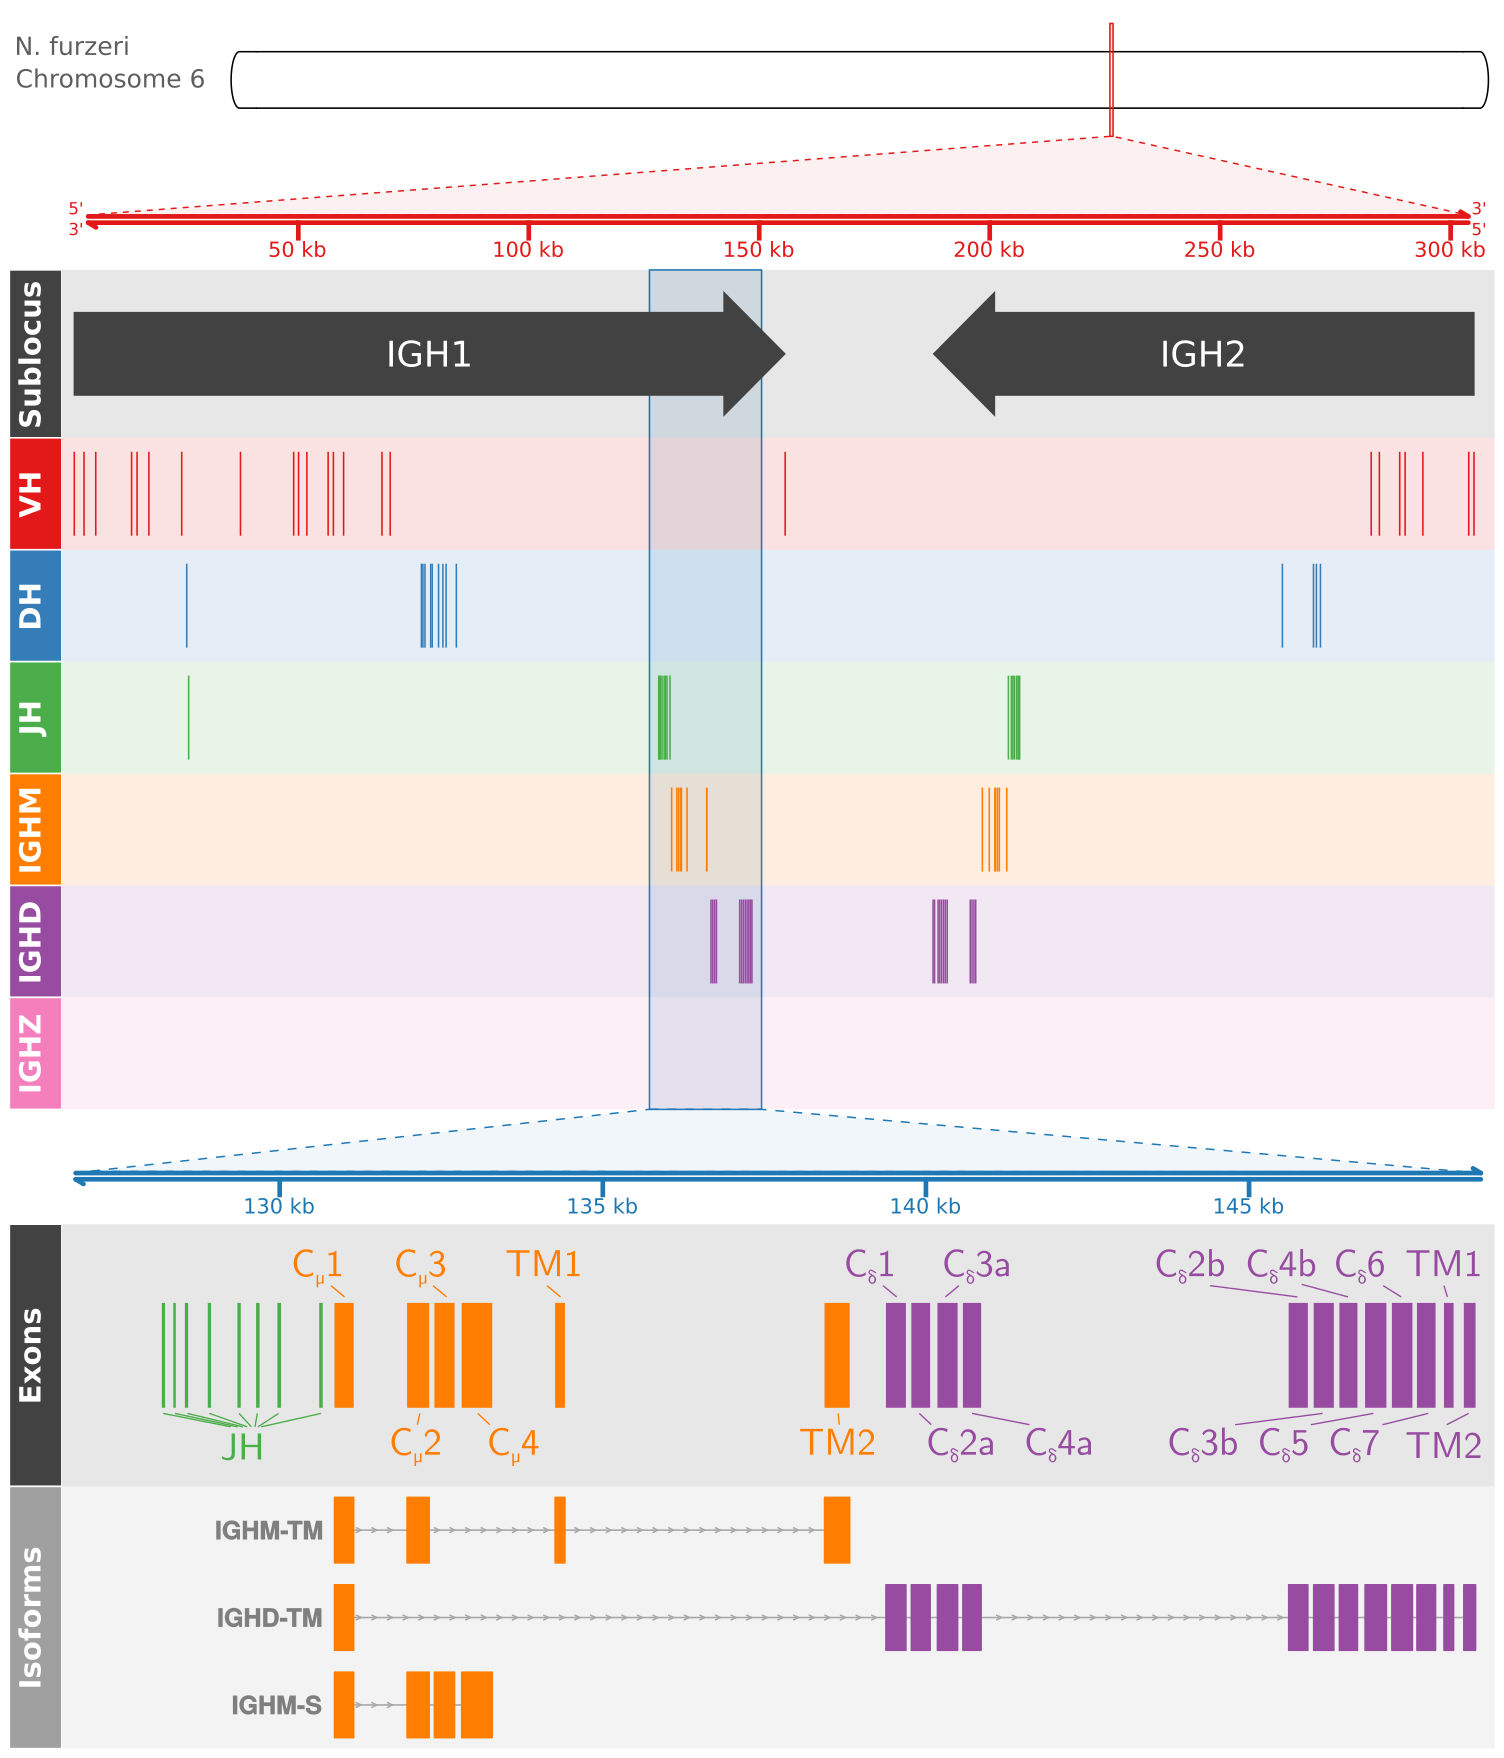
\includegraphics[width=\textwidth]{/home/will/Documents/code/figures/2018-11-06/nfu-locus-map_small} % TODO: Move to thesis directory, switch to large figure
			    \begin{subfigure}{0em}
        \phantomsubcaption{}
        \label{fig:nfu-locus-map-a}
    \end{subfigure}
    \begin{subfigure}{0em}
        \phantomsubcaption{}
        \label{fig:nfu-locus-map-b}
    \end{subfigure}
    \begin{subfigure}{0em}
        \phantomsubcaption{}
        \label{fig:nfu-locus-map-c}
        \end{subfigure}
	\caption[The immunoglobulin heavy chain (\textit{IGH}) locus in \textit{Nothobranchius furzeri}]{\textbf{The immunoglobulin heavy chain (\textit{IgH}) locus in \textit{Nothobranchius furzeri}:} (A) Position of the \textit{IgH} locus on chromosome 6 of the \Nfu genome. (B) Arrangement of \vh, \dh, \jh and constant-region gene segments on the \Nfu \textit{IgH} locus. All segments follow the orientation of their parent sublocus, indicated in the uppermost track. (C) Detailed map of the constant regions of the \textit{IGH1} sublocus, indicating the position and identity of the constant-region exons and the exon composition of expressed \textit{IgH} isoforms in the turquoise killifish.}
	\label{fig:nfu-locus-map}
	\end{figure}
	
	\begin{figure}
	\centering
	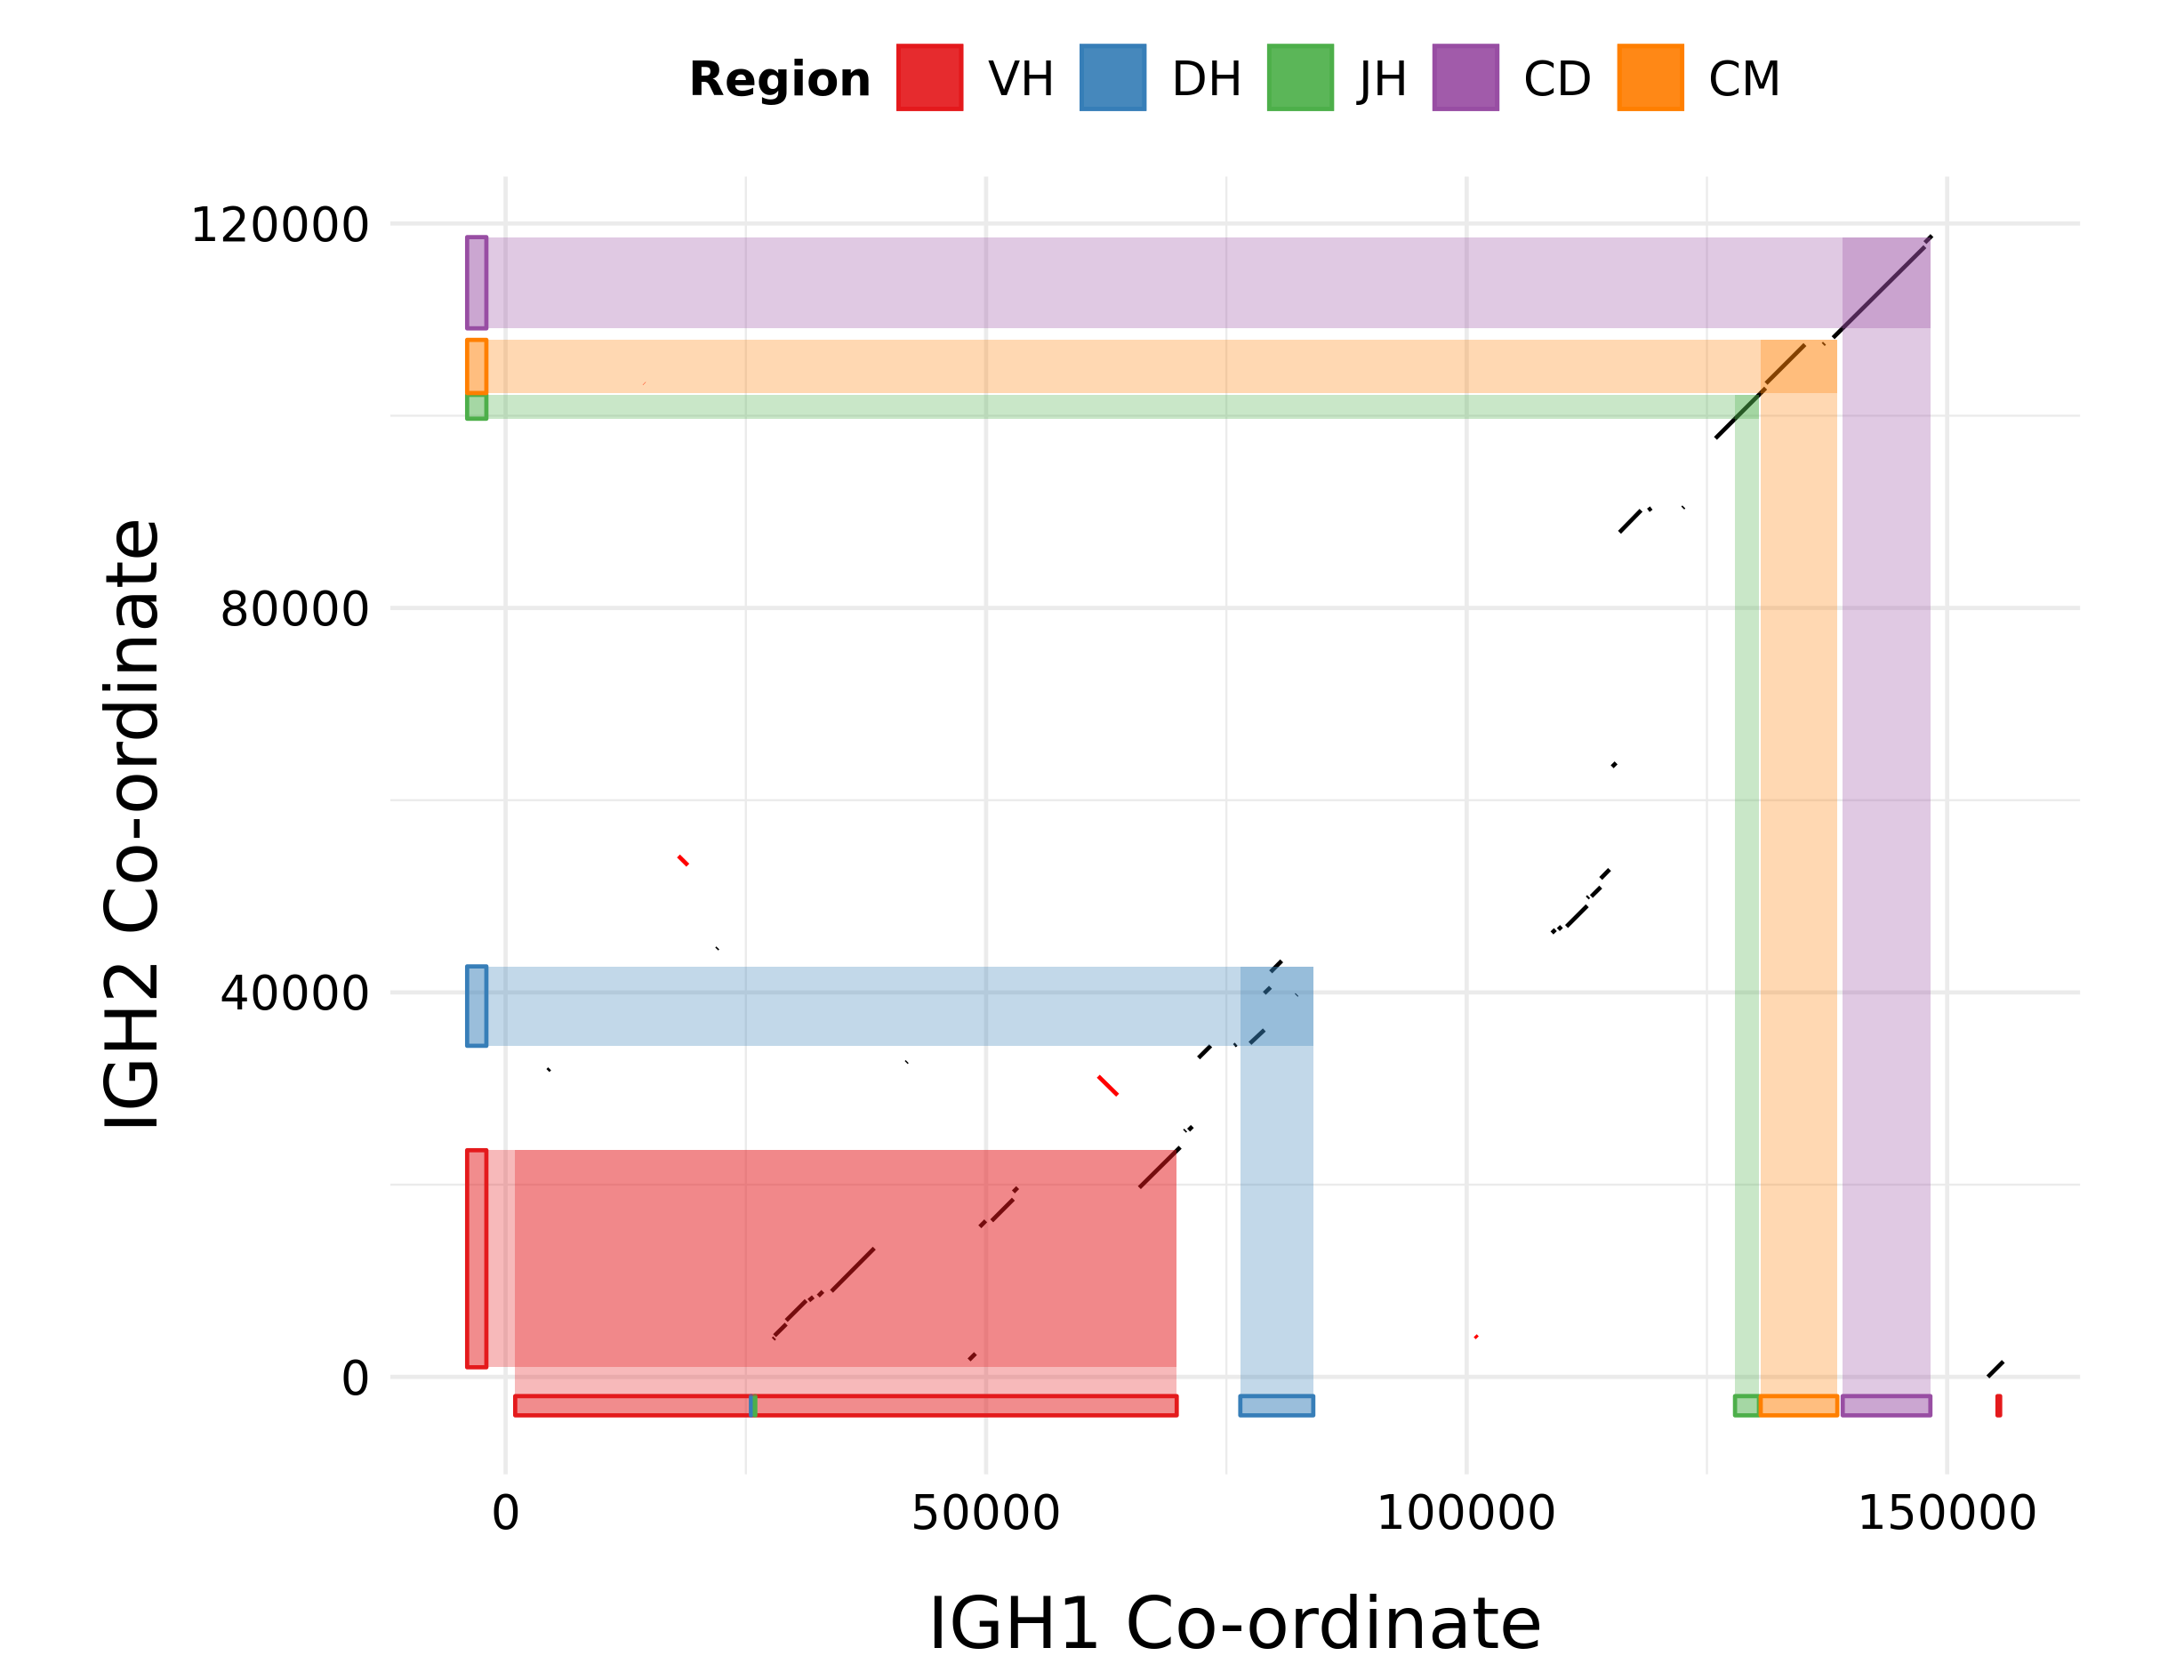
\includegraphics[width=0.9\textwidth]{_Figures/png/nfu-locus-dots.png}
	\caption[Sequence homology between subloci in \Nfu \textit{IGH}]{\textbf{Sequence homology between subloci in \Nfu \textit{IGH}:} Synteny plot of sequential best matches between \textit{IGH1} and \textit{IGH2} subloci, with gene segment regions indicated by coloured rectangles along each axis.}
	\label{fig:nfu-locus-synteny}
	\end{figure}
	
	\subsection{Constant regions}
	\label{sec:nfu-locus-constant}
	
	The isotype (also known as the class) of an antibody determines its functional role within the immune system, including its possible effector functions and whether it can be secreted. Three antibody isotypes have been identified to date in teleost fishes: IgM, IgD and IgZ (a.k.a. IgT, IgT/Z or IgZ/T). Of these, IgM and IgD are highly primitive within the jawed vertebrates and found in most or all other vertebrate groups; within the teleosts, both appear to be universal. Conversely, IgZ is a teleost-specific isotype which is absent in other vertebrate taxa; within the teleosts, most characterised exons possess IgZ, but at least two (medaka and channel catfish) have been found to lack it. In rainbow trout, IgZ has been found to play a specialised mucosal role in the immune system analagous to that of IgA in mammals, and it is widely assumed to play this specialised role throughout the teleosts; it is as yet unclear how mucosal immunity is effected in species lacking IgZ.
	
	IgM, the most primitive and widely-found isotype in jawed vertebrates, is present immediately downstream of the main \jh-region and occupies the standard six-exon configuration, with four \cm{} exons and two transmembrane domains present in series on the chromosome (\Cref{fig:nfu-locus-map-b,fig:nfu-locus-map-c,fig:teleost-igm-exons-a}). As with other species, both secreted and transmembrane isoforms of IgM are present in the transcriptome, with secreted IgM consisting of \cm{1-4} (\Cref{fig:nfu-locus-map-c,fig:nfu-locus-sashimi-a,fig:teleost-igm-exons-b}); however, the exon configuration of transmembrane IgM deviates from both that seen in mammals (in which exon TM1 is spliced to a cryptic splice site within \cm{4}) and most teleosts (in which the canonical splice site following \cm{3} is used and \cm{4} is excised). Rather, TK IgM-TM resembles that of medaka, in which both \cm{3} and \cm{4} are excluded and the canonical splice site at the end of \cm{2} is spliced directly to TM1 (\Cref{fig:teleost-igm-exons-c,fig:teleost-igm-exons-d,fig:teleost-igm-exons-e}). The similarity to medaka, which again is the closest relative of TK with a characterised locus, raises the possibility that this unusual splicing behaviour may be a conserved feature of both lineages; however, the underlying mechanism giving rise to this difference in splicing behaviour is unknown.
	
		Unlike IgM, the exon structure of IgD is highly variable across the teleosts, ranging from roughly 7-17 \cd{} exons in addition to the transmembrane domains. The core structure of IgD comprises seven \cd{} exons (\cd{1-7}), but some subset of these exons may be missing or duplicated in any given species -- in medaka, for example, \cd{5} is missing in all subloci, while in many species (e.g. zebrafish, salmon, and channel catfish) \cd{2-4} are duplicated in two or more tandem blocks. This latter configuration is a in turquoise killifish, in which the IgD constant region immediately follows IgM in both subloci and has a 

\cd{1}-(\cd{2}-\cd{3}-\cd{4})$_2$-\cd{5}-\cd{6}-\cd{7}-TM1-TM2 

	\noindent configuration, for a total of 12 exons per IgD constant region (\Cref{fig:nfu-locus-map-b,fig:nfu-locus-map-c}). All of these exons appear to be expressed in tandem, resulting in a much longer IgH transcript than is observed for any isoform of IgM (\Cref{fig:nfu-locus-map-c,fig:nfu-locus-sashimi-b}). Of the duplicated exon pairs, \cm{3}A/B and to a lesser extent \cm{4}A/B are highly similar, while \cm{2}A/B are more distinct (\Cref{fig:nfu-ch-aln}). As in other teleost species, IgD in the turquoise killifish includes a chimeric \cm{1} exon at the 5' end of the constant-region transcript, for a total of 13 exons per IgD-TM mRNA (\Cref{fig:nfu-locus-sashimi-b}).

	While the best-known form of IgD in teleosts is transmembrane, secreted IgD has been observed in at least two teleost species, with different mechanisms used in each case: in channel catfish, one dedicated sublocus has a dedicated IgD secretory exon in place of the transmembrane exons, while in rainbow trout (and possibly some other species like Atlantic salmon and cod) a run-on event at the end of \cd{7} results in the production of a secretory tail in a manner similar to secretory IgZ. However, neither a specialised secretory exon nor a \cd{7} secretory tail could be detected in turquoise killifish, suggesting that IgD may only be expressed in transmembrane form in this species. % TODO: Figure comparing post \cd{7} sequence in trout, salmon, cod and TK (and other species from paper?) to demonstrate lack of secretory tail in TK
	
	In the case of both IgM and IgD, the constant regions are present in their expected configuration in each sublocus and are highly similar in sequence between the subloci, with an average of 98.4\% nucleotide sequence identity for corresponding IgM exons and 99.3\% for corresponding IgD exons (\Cref{fig:nfu-ch-aln} and \Cref{tab:nfu-ch-aln}).

	The most striking feature of the constant-region structure of the \textit{IGH} locus in \Nfu is the complete absence in both subloci of IgZ. As discussed above, IgZ constant exons have been found to be present in the great majority of teleost \textit{IgH} loci characterised to date, with the only previous exceptions being channel catfish and medaka. Its absence in turquoise killifish (\Cref{fig:nfu-locus-map-b}) is therefore notable, and immediately raises questions about the nature, kinetics and efficacy of mucosal adaptive immunity in this species. Since medaka, the closest relative of TK with a characterised locus, also lacks IgZ, its absence in TK also raises the question of whether its absence occurred in a common ancestor to both species or is the result of independent deletion events in both lineages; this question is addressed in more depth in subsequent sections of this chapter. % IgZ paragraph at start or end of subsection?	

	% TODO: Table and figure of antibody isoforms in TK: length, molecular weight, number of C-regions, etc. (in appendix)
	
	\begin{figure}
	\centering
		    \begin{subfigure}{0em}
        \phantomsubcaption{}
        \label{fig:teleost-igm-exons-a}
    \end{subfigure}
    \begin{subfigure}{0em}
        \phantomsubcaption{}
        \label{fig:teleost-igm-exons-b}
    \end{subfigure}
    \begin{subfigure}{0em}
        \phantomsubcaption{}
        \label{fig:teleost-igm-exons-c}
    \end{subfigure}
    \begin{subfigure}{0em}
        \phantomsubcaption{}
        \label{fig:teleost-igm-exons-d}
    \end{subfigure}
    \begin{subfigure}{0em}
        \phantomsubcaption{}
        \label{fig:teleost-igm-exons-e}
    \end{subfigure}
	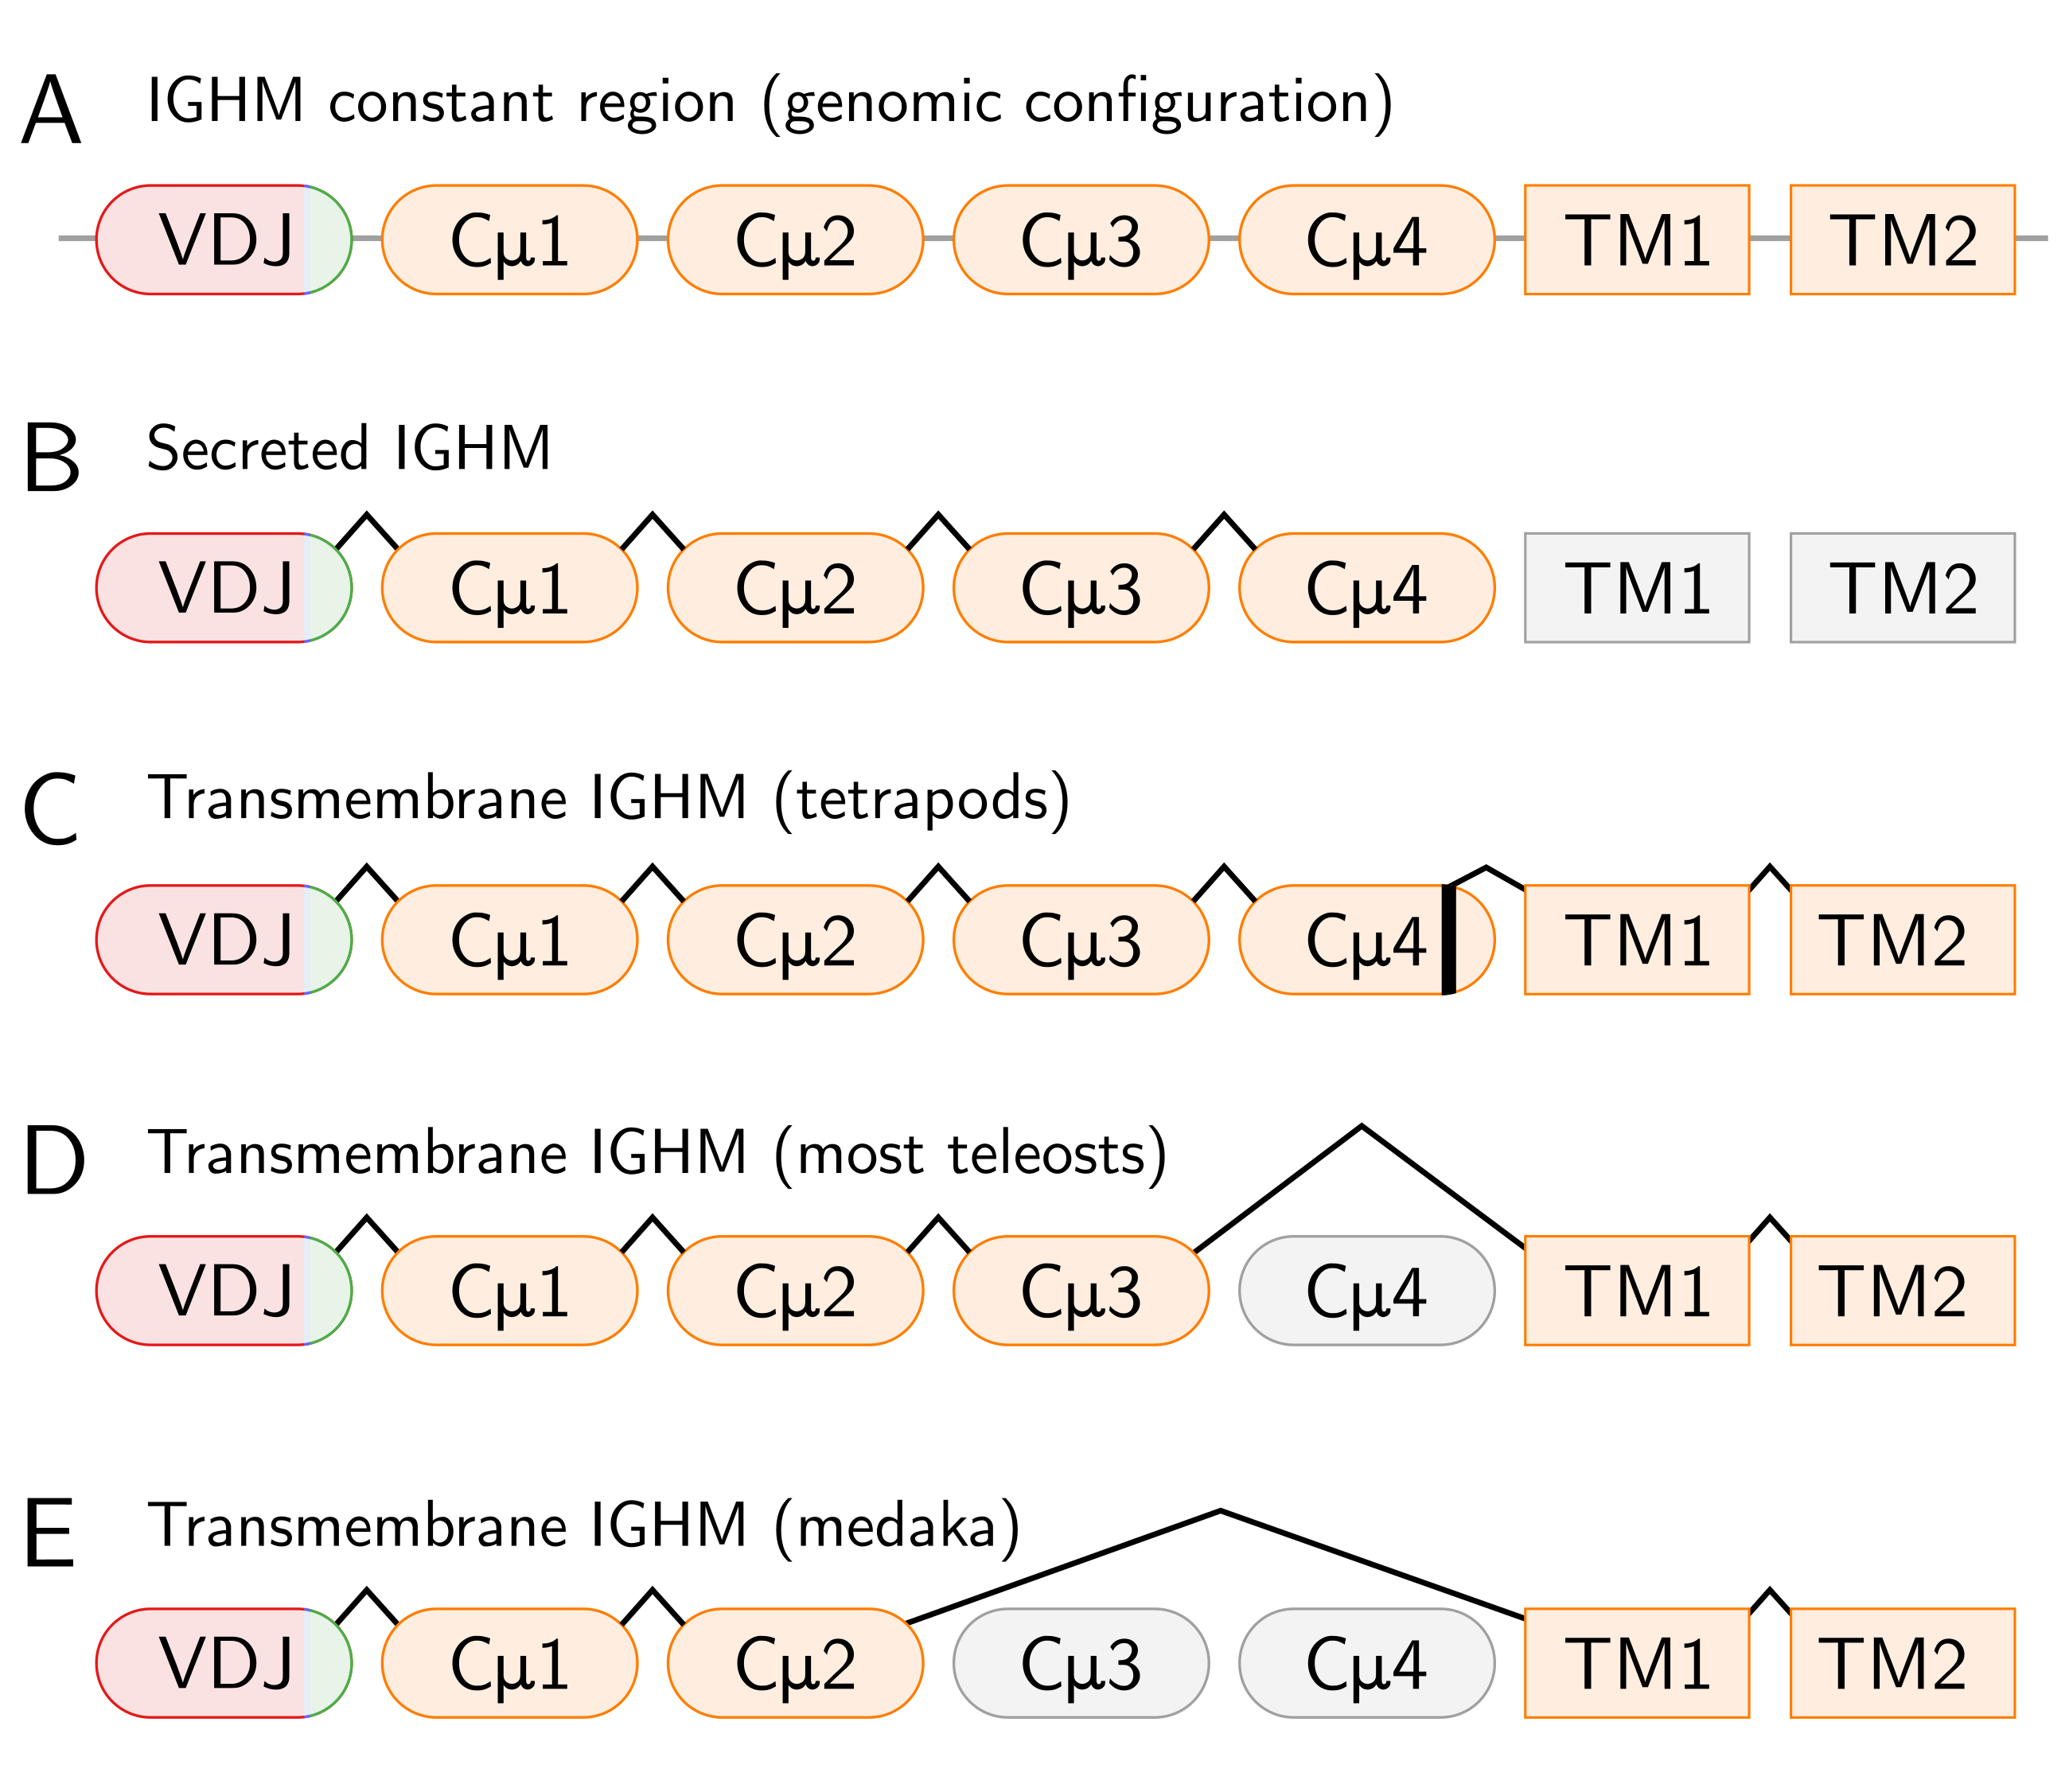
\includegraphics[width=0.8\textwidth]{_Figures/png_edited/teleost-igm-exons}
	\caption[IgM exon usage in other vertebrates]{\textbf{IgM exon usage in other vertebrates:} Schematic of IgM splice patterns in different isoforms and taxonomic groups; (A) standard genomic (pre-splicing) configuration of IgM, following VDJ recombination; (B) exon configuration of secreted IgM (IgM-S) in tetrapods and teleosts; (C) exon configuration of transmembrane IgM (IgM-TM) in tetrapods, demonstrating the use of a cryptic splice site in \cm{4}; (D) standard IgM-TM exon configuration in teleosts, demonstrating the direct splicing of \cm{3} to TM1 and exclusion of \cm{4}; (E) unusual IgM-TM exon configuration observed in medaka, in which both \cm{3} and \cm{4} are excluded. Figure adapted from Fillatreau \textit{et al.} (2013).}
	\label{fig:teleost-igm-exons}
	\end{figure}
	
	\begin{figure}
	\centering
		\begin{subfigure}{0em}
        \phantomsubcaption{}
        \label{fig:nfu-locus-sashimi-a}
    \end{subfigure}
    \begin{subfigure}{0em}
        \phantomsubcaption{}
        \label{fig:nfu-locus-sashimi-b}
    \end{subfigure}
	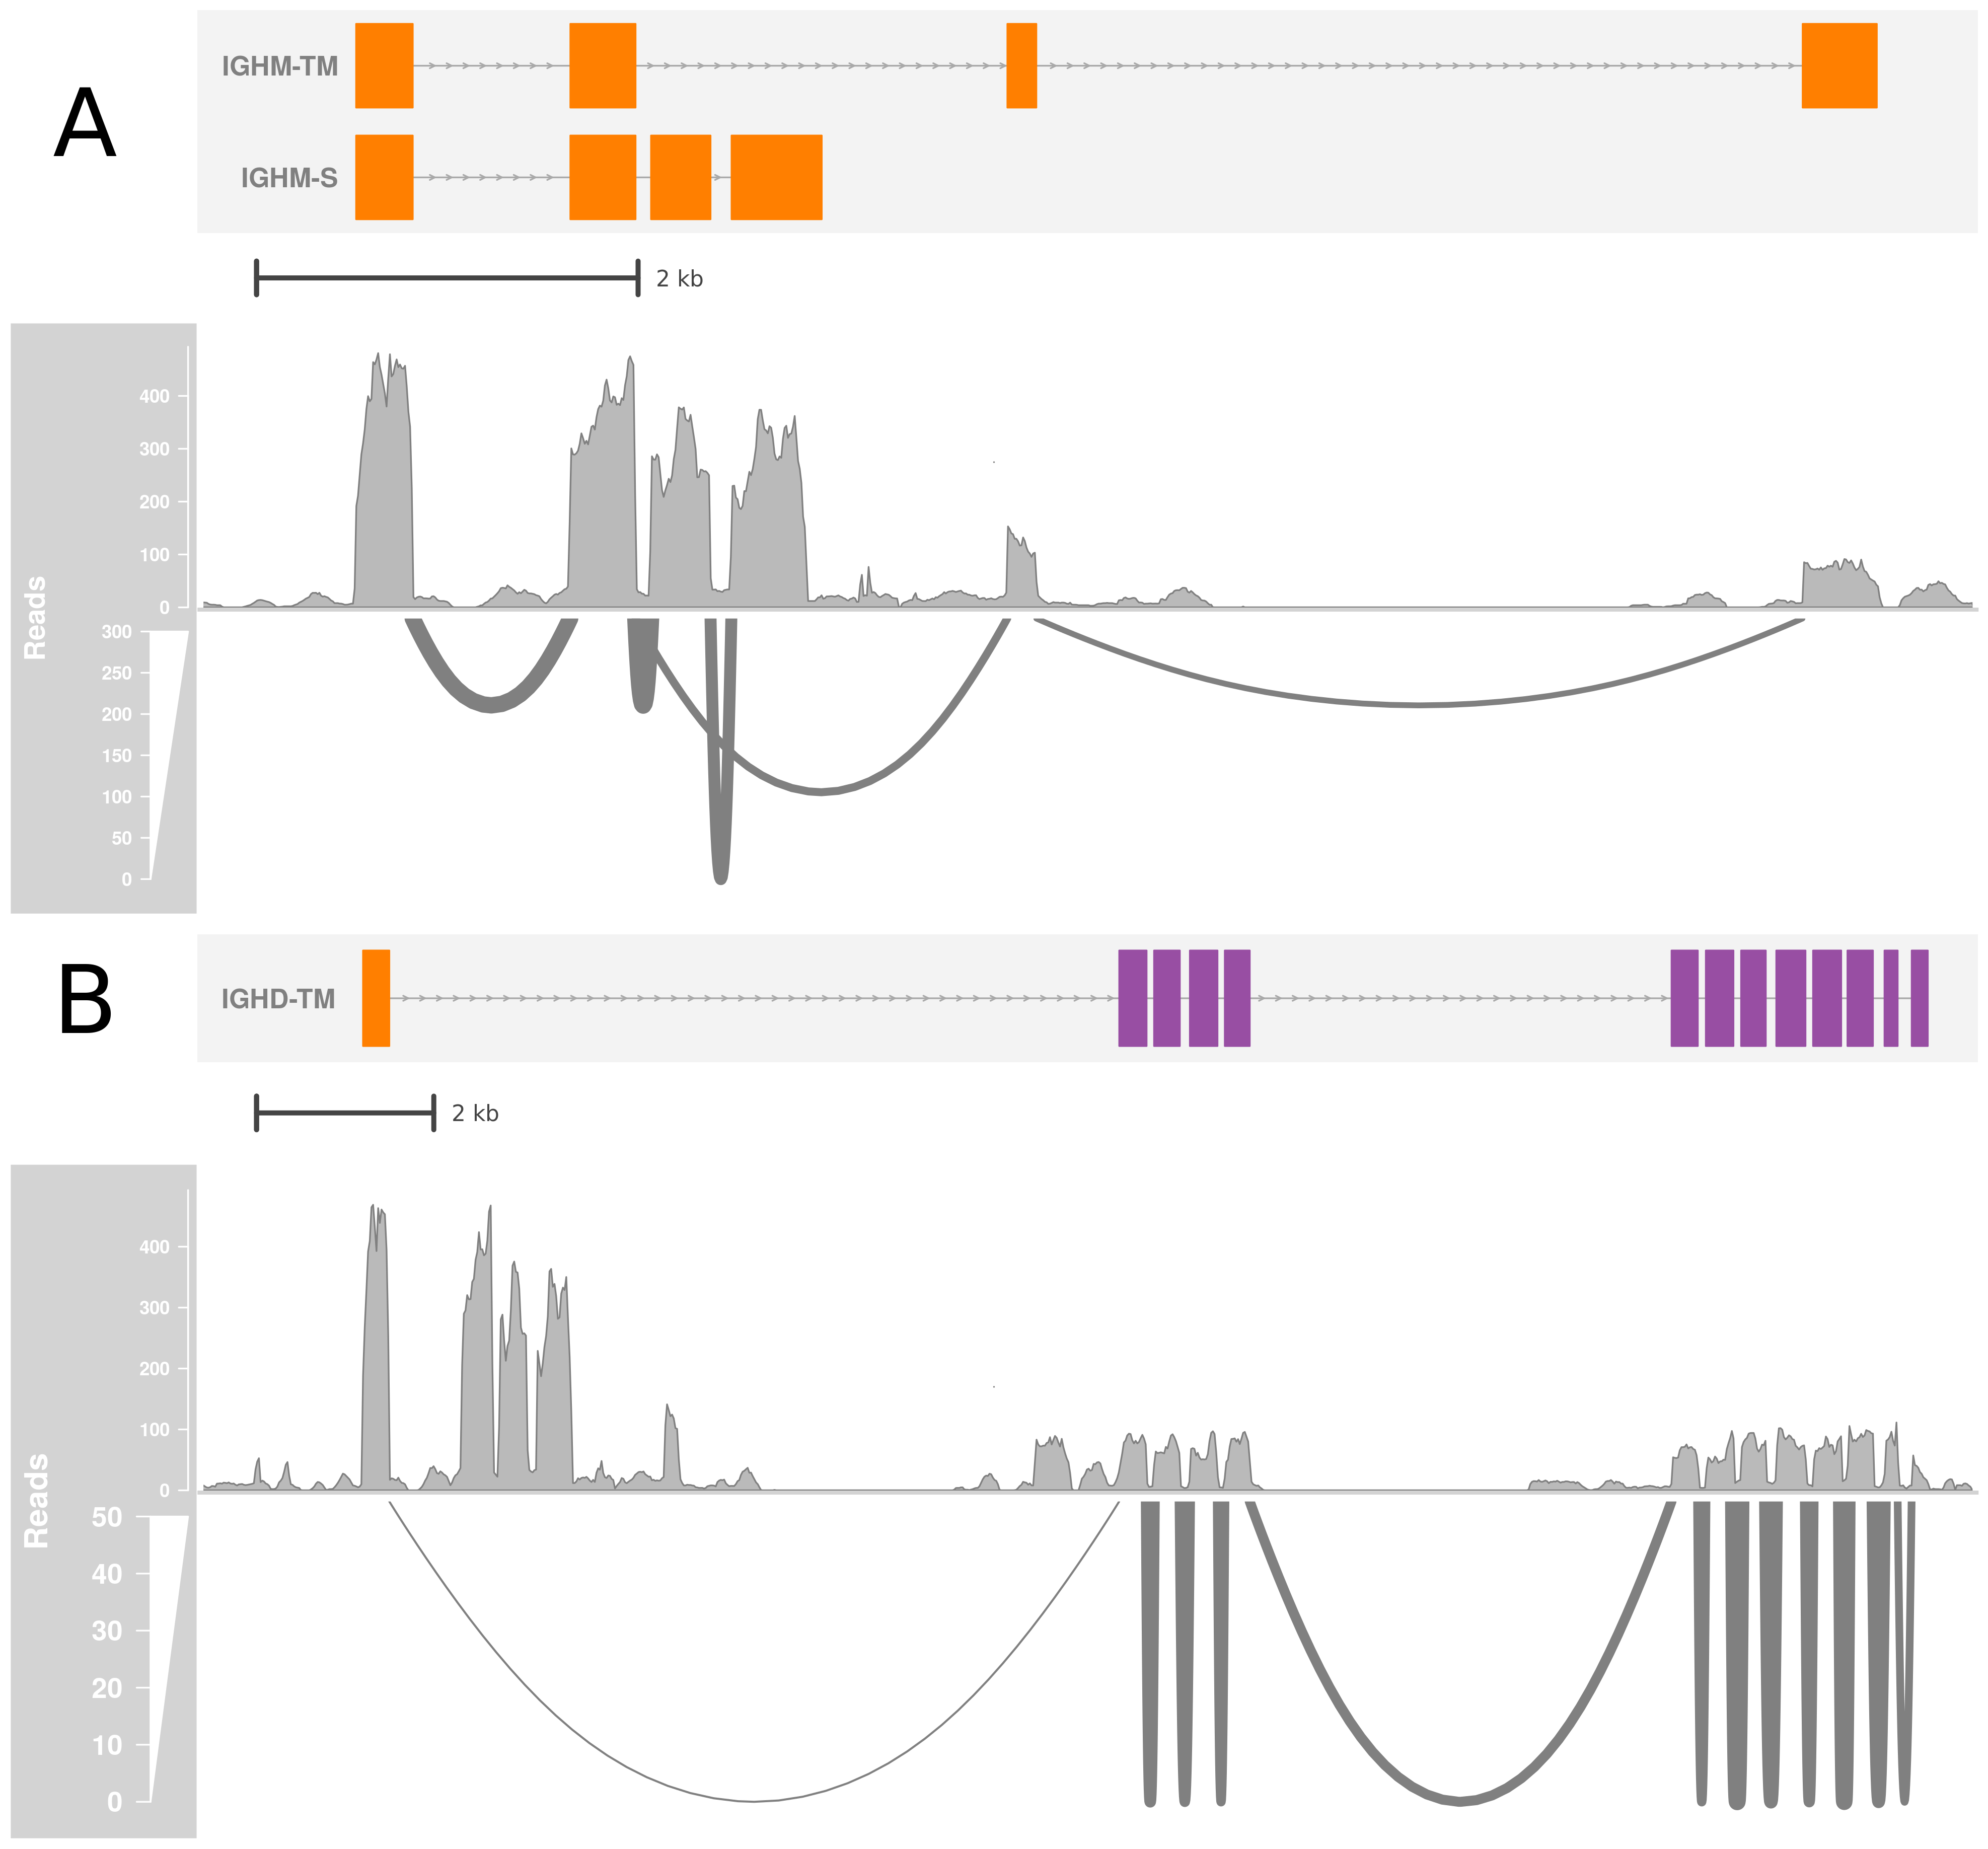
\includegraphics[width=\textwidth]{_Figures/png/nfu-locus-sashimi}
	\caption[Constant-region isoforms in \Nfu]{\textbf{Constant-region isoforms in \Nfu:} Coverage and sashimi plots of STAR-aligned RNA-seq reads from \Nfu gut samples, demonstrating the splicing behaviour of IGH1 constant-region isoforms. (A) IGHM exon splicing, showing alternative splicing patterns of IGHM-TM and IGHM-S; (B) IGHD exon splicing, including splicing of \cm{1} to \cd{1}.}
	\label{fig:nfu-locus-sashimi}
	\end{figure}
	
	\begin{figure}
	\centering
	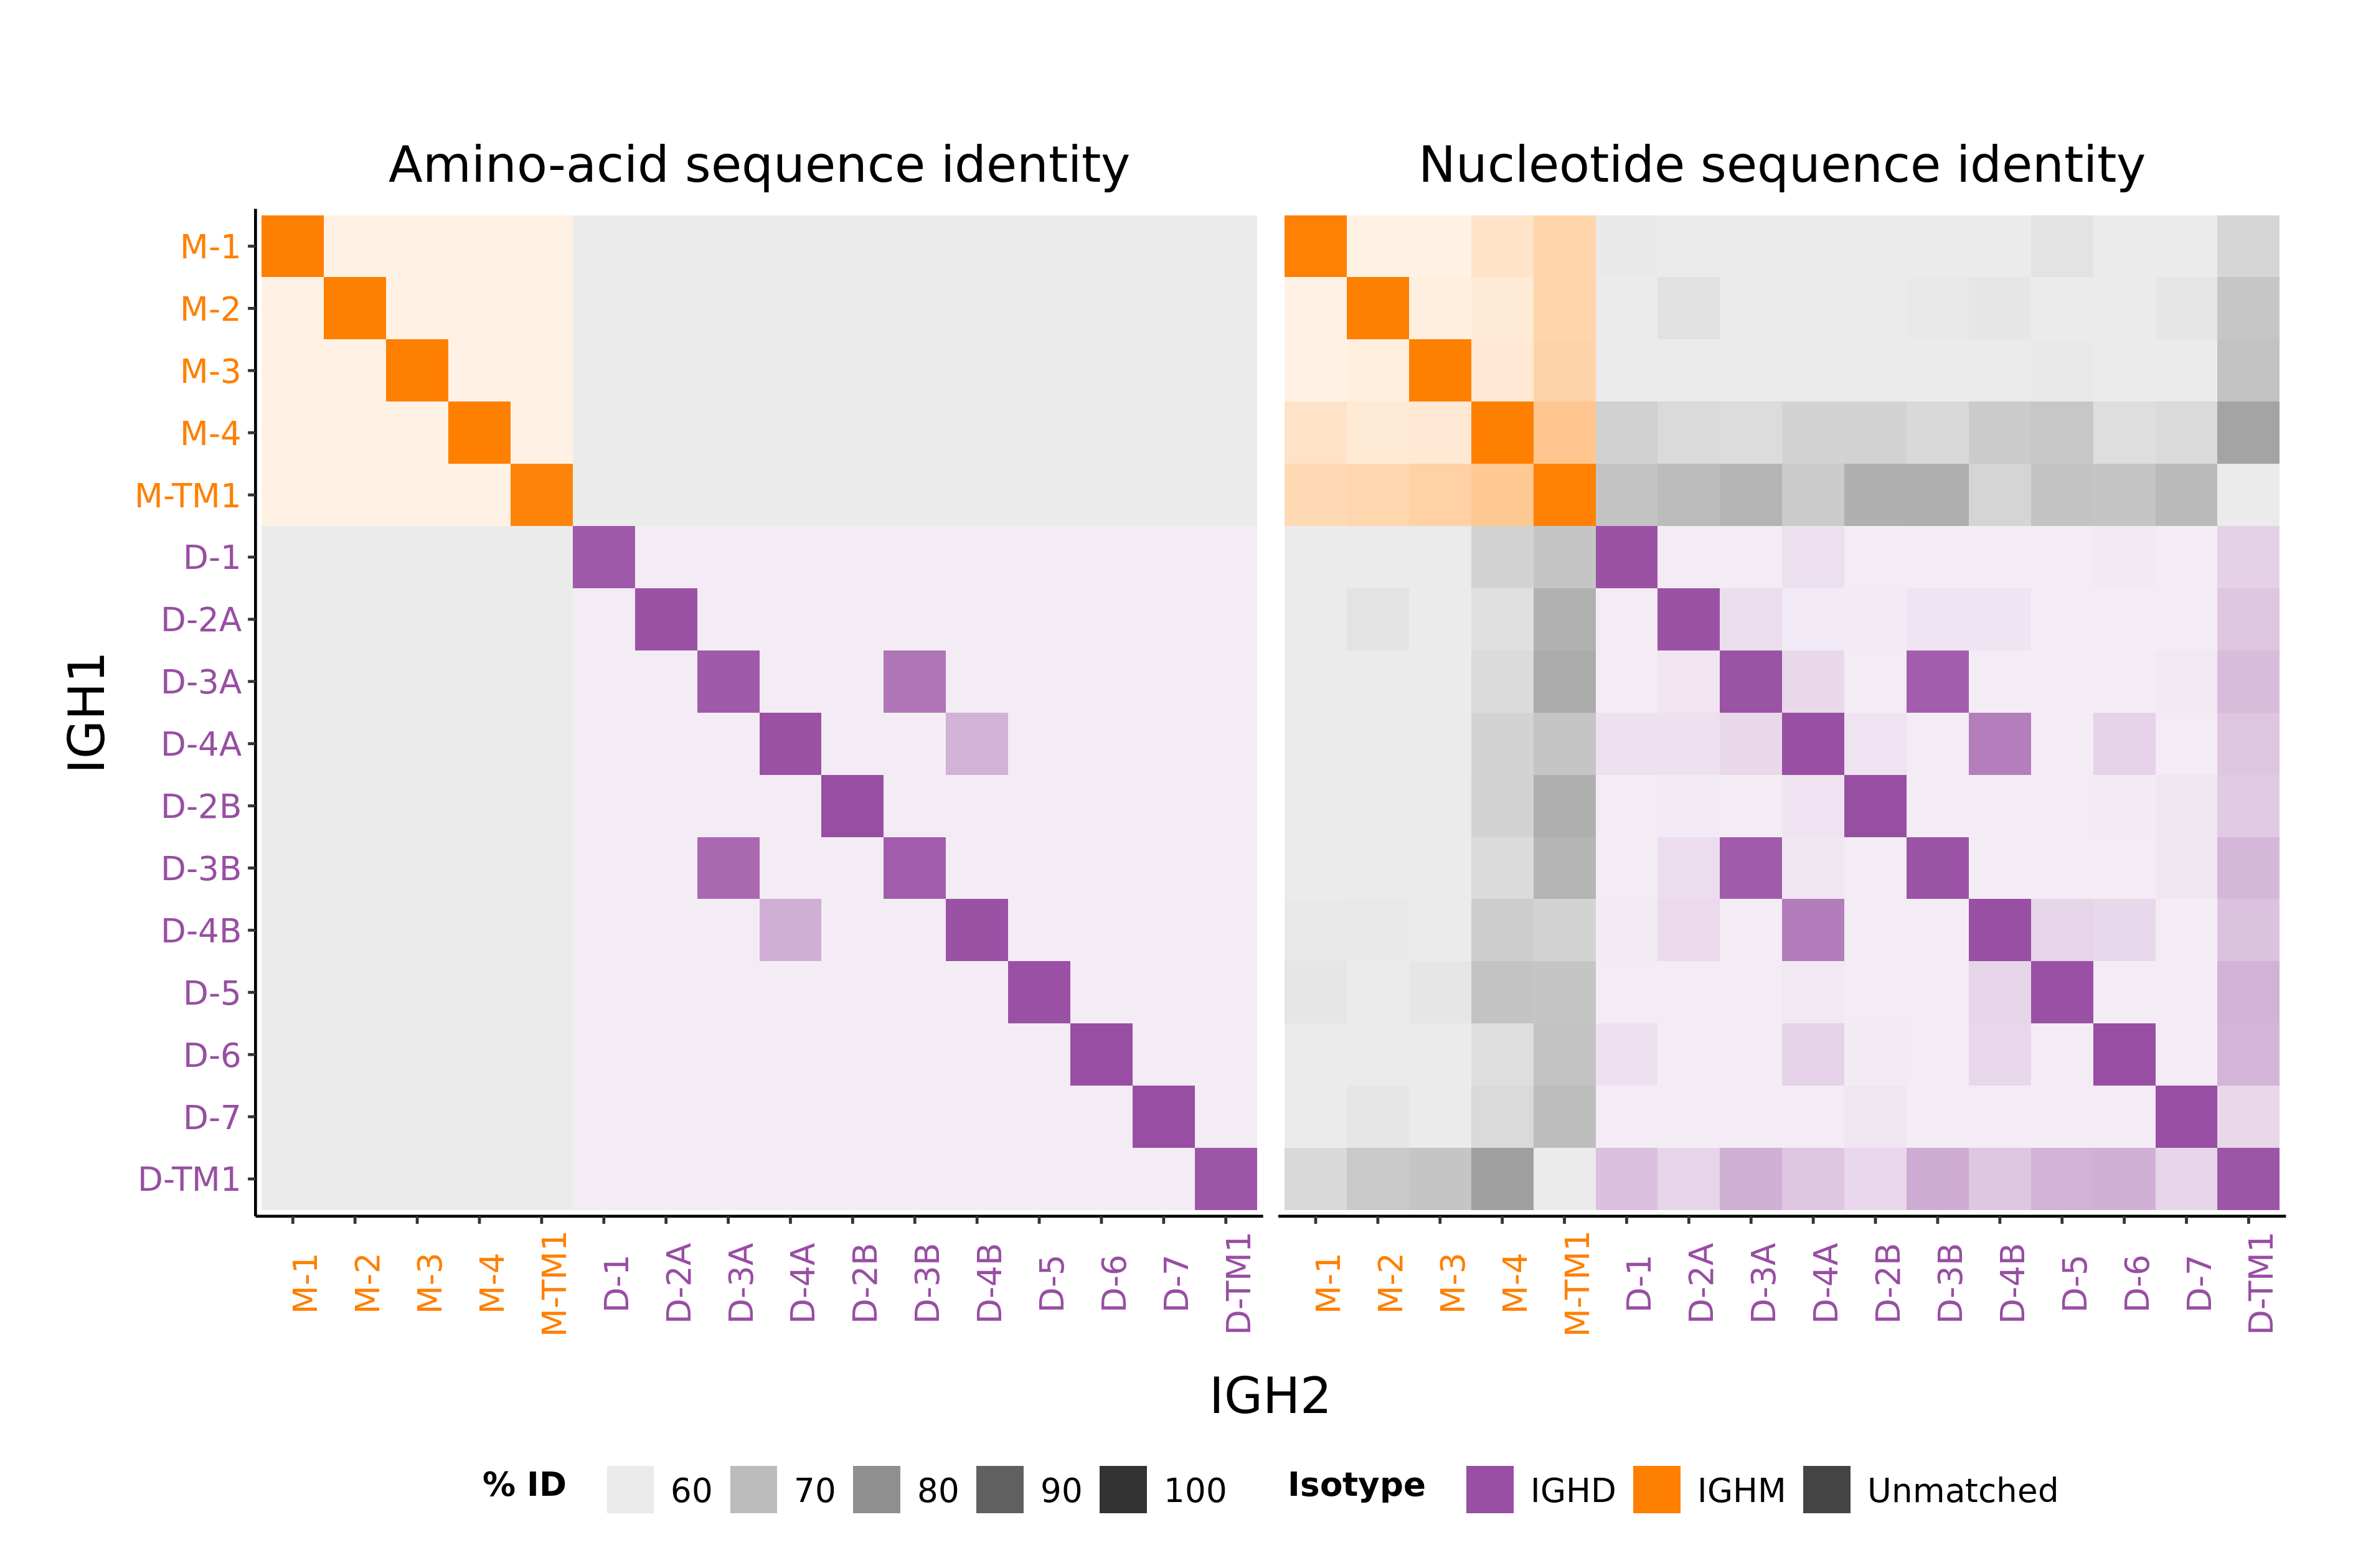
\includegraphics[width = \textwidth]{_Figures/png/nfu-ch-aln}
	\caption[Cross-sublocus sequence similarity in constant-region exons in \Nfu \textit{IGH}]{\textbf{Cross-sublocus sequence similarity in constant-region exons in \Nfu:} Heatmap of percentage sequence identity between amino-acid (right) and nucleotide (left) sequences of constant-region exons (excluding IGHM-TM2 and IGHD-TM2) from the two subloci of \Nfu \textit{IGH}, calculated using pairwise Needleman-Wunsch global alignments. Note the very high similarity between corresponding exons of the two subloci, as well as the substantial similarity between IGHD-3A/3B and IGHD-4A/4B in both subloci.}
	\label{fig:nfu-ch-aln}
	\end{figure}
	
	\begin{table}\centering
		\caption[Cross-sublocus sequence similarity between corresponding constant-region exons in \Nfu \textit{IGH}]{\textbf{Cross-sublocus sequence similarity in constant-region exons in \Nfu:} Percentage sequence identities of pairwise Needleman-Wunsch global alignments between nucleotide (NT) or amino-acid (AA) sequences of corresponding exons from the two subloci of \Nfu \textit{IGH}.}
	% latex table generated in R 3.5.1 by xtable 1.8-3 package
% Wed Dec 19 17:33:43 2018
\begin{tabular}{llrr}
  \toprule Isotype & Exon & NT & AA \\ 
  \midrule M & 1 & 99.66 & 100.00 \\ 
  M & 2 & 100.00 & 100.00 \\ 
  M & 3 & 100.00 & 100.00 \\ 
  M & 4 & 100.00 & 100.00 \\ 
  M & TM1 & 99.34 & 98.00 \\ 
  M & TM2 & 91.67 & 100.00 \\ 
  D & 1 & 99.03 & 97.06 \\ 
  D & 2A & 98.97 & 98.96 \\ 
  D & 3A & 98.72 & 97.09 \\ 
  D & 4A & 99.65 & 98.92 \\ 
  D & 2B & 100.00 & 100.00 \\ 
  D & 3B & 98.72 & 96.12 \\ 
  D & 4B & 99.64 & 98.91 \\ 
  D & 5 & 99.09 & 99.08 \\ 
  D & 6 & 100.00 & 100.00 \\ 
  D & 7 & 100.00 & 100.00 \\ 
  D & TM1 & 97.99 & 97.96 \\ 
  D & TM2 & 99.44 & 100.00 \\ 
   \bottomrule \end{tabular}

	\label{tab:nfu-ch-aln}
	\end{table}
	




	\subsection{Variable regions}
	\label{sec:nfu-locus-variable}
	
	\subsubsection{Organisation, functionality and diversity}
	\label{sec:nfu-locus-variable-orga}
	 
	% Presence and functionality
	In total, 24 \vh-segments, 14 \dh-segments and 17 \jh-segments were identified in the \Nfu locus, of which the majority (17 \vh, 10 \dh and 8 \jh) were present in \textit{IGH1}. Of the \vh segments identified, three contain premature STOP codons, though none is out-of-frame; conversely, all the \dh and \jh segments identified appear to be in-frame and functional, with no premature STOP codons. However, in all cases a minority of segments contain RSS sequences that deviate significantly from the expected consensus sequence; it is unclear whether these sequences can recombine to successfully produce mature VDJ sequences \textit{in vivo}. In the case of the \vh segments, of the six sequences without clearly functional RSS sequences, three also contain premature STOP codons, suggesting the changes to the RSS in these cases may arise from relaxed purifying selection on already-pseudogenised sequences.
	
	% Location and exceptions
	Of the \vh, \dh and \jh segments identified, all but one of each type of segment is located within contiguous V-, D-, and J-regions within each sublocus, supporting a modified translocon configuration for killifish \textit{IGH}. The exceptions to this are IGH1D01 and IGH1J01, which are embedded within the IGH1 V-region, and a single \vh segment located in between the IGHD contant regions of the two subloci (\Cref{fig:nfu-locus-map-b}). The unusual location of IGH1D01 and IGH1J01 may represent the result of a transposition event within the IGH locus; however, their close colocalisation and 5' position within the IGH1 sublocus, as well as the fact that neither has a close paralogue in IGH2 (\Cref{fig:nfu-dj-alignment-b}), suggest that they may alternatively represent the remnant of a formerly present IGHZ constant region, as these typically have dedicated D/J segments independent of those serving IGHM. Given its forward orientation, meanwhile, the orphaned \vh-segment was assigned to the IGH1 sublocus as IGH1V1-07; however, if annotated correctly, it is unlikely to successfully recombine with segments in either sublocus due to its unusual location. % Alternatively, the unusual location of this \vh segment could be due to either a misassembly or the presence of an additional sublocus missing from the current assembly; however, given the structurally volatile nature of the IGH locus and the frequency with which isolated \vh loci are found in other parts of the genome, the presence of an orphaned locus in between two functional subloci is not implausible.
		
	% Segment numbers
	The total number of functional \vh segments in the killifish locus is unusually small in comparison to the total numbers observed in many other teleost species (\Cref{tab:teleost-vh-counts}); however, the number of segments per sublocus is in line with the numbers seen in closely-related species (2 to 12 in medaka, 6 to 18 in stickleback), with the overall difference mainly arising from a difference in the number of subloci per locus. A similar pattern is observed with \dh and \jh segments, with similar numbers of segments per sublocus in killifish and closely-related species, especially medaka. It therefore appears that the per-sublocus segment diversity available to the turquoise killifish is similar to that of previously characterised species, with any difference in total available diversity at this level arising from differences in the number of functional subloci rather than the size of the V/D/J-regions \textit{per se}.
	
	\begin{table}
	\begin{threeparttable}
	\caption{\textbf{Number of functional \vh-segments and \vh-families in other teleost species}}
	\label{tab:teleost-vh-counts}
	\begin{tabular}{ccccc}\toprule
	\textbf{Common Name} & \textbf{Species} & \textbf{\# Functional \vh Segments} & \textbf{\# \vh Families} & \textbf{Source}\\\midrule
	Zebrafish & \textit{Danio rerio} & 39 & 13\,\tnote{1} & Magadan 2015 \\
	Grasscarp & \textit{Ctenopharyngodon idella} & 8 & 5\,\tnote{2} & Xiao 2010 \\
	Fugu & \textit{Takifugu rubripes} & 34 & 3 & Magadan 2015 \\
	Medaka & \textit{Oryzias latipes} & 35 & 6 & Fillatreau, Magadan 2011 \\
	Stickleback & \textit{Gasterosteus aculeatus} & 49 & 4 & Magadan 2015 \\
	Turquoise killifish & \textit{Nothobranchius furzeri} & 21\,\tnote{3} & 6 & -- \\
	\bottomrule\end{tabular}
	\begin{tablenotes}
	\item[1] \vh families in zebrafish identified based on 70\% (rather than 80\%) sequence identity.
	\item[2] It is not clear what clustering method or threshold was used to identify \vh families in grasscarp.
	\item[3] Excluding \vh segments with nonsense or frameshift mutations, but not those with uncertain or missing RSS sequences.
	\end{tablenotes}
	\end{threeparttable}
	\end{table} % TODO: Convert source labels into proper citations
	
	\subsubsection{Sublocus synteny and evolution}
	\label{sec:nfu-locus-variable-synteny}

	% Synteny
		As can be seen from \Cref{fig:nfu-locus-synteny}, much of the V-, D- and especially J-region sequence in the \Nfu locus is syntenic between the two \textit{IGH} subloci, with downstream portions of the \textit{IGH2} V-region corresponding to downstream parts of the \textit{IGH1} region (after correcting for locus orientation). Of the seven \vh segments in \textit{IGH2}, six have a correspending segment on \textit{IGH1} with which they share at least 97\% sequence identity (\Cref{fig:nfu-vh-families}), and these partner segments are largely (but not entirely) colinear in their ordering between the two subloci. A similar pattern can be observed for the D- and (especially) the J-regions: of the four \dh segments detectable in IGH2, three (IGH2D02 to IGH2D04) are identical with another block of adjacent \dh segments in IGH1 (IGH1D05 to IGH1D07), while the the J-regions exhibit almost complete sequence identity between the eight \jh segments of the main \jh region in IGH1 and the eight \jh segments in IGH2 (\Cref{fig:nfu-dj-alignment}).
		
		Nevertheless, as is clear from \Cref{fig:nfu-locus-synteny}, there are large portions the \textit{IGH1} variable region, including the first 25 kilobases of the V-region, for which no corresponding sequence exists in \textit{IGH2}, and there are many \vh and \dh segments in IGH1 (and a much smaller number in IGH2) for which no close homologue exists in the other sublocus. Taken together, these data are consistent with a model in which \textit{IGH2} was produced via duplication and inversion of all or part of \textit{IGH1}, followed by subsequent deletion events in the redundant, and structurally volatile, \textit{IGH2} \vh and \dh regions. However, it is not clear at present how to distinguish between this model and an alternative one of expansion in IGH1, explain why IGH2 and IGH1 should have undergone deletion events, or identify why the \jh region is so much more conserved between subloci than either the \vh or \jh regions.
% TODO: Think about these questions, try to suggest hypotheses
		

	\subsubsection{\vh families}
	\label{sec:nfu-locus-variable-families}
	
	\vh sequences within an \textit{IGH} locus are conventionally grouped into families on the basis of nucleotide sequence identity, with a typical identity cutoff of 80\%. In order to group the \Nfu \vh genes into families, pairwise Needleman-Wunsch global alignments were performed on each pair of \vh sequences to obtain pairwise identity scores, followed by single-linkage clustering on the resulting identity matrix. Cutting the dendrogram at 80\% sequence identity revealed a total of six \vh families, of which four contained more than one \vh segment (\Cref{fig:nfu-vh-families}). 	V2 and V4 are highly similar and all the members of V4 are pseudogenised by premature STOP codons; it may therefore be better to regard V4 as a pseudogenised subfamily of V2 than a \vh family in its own right. Of the remaining families, V1 and V2 make up the bulk (42\% and 29\% respectively) of the \vh segments in the locus. 
	
	The number of \vh families is roughly in line with those found in related species (\Cref{tab:teleost-vh-counts}), indicating that, while the total number of \vh segments in the turquoise killifish may be unusually low (see \Cref{sec:nfu-locus-variable-orga}), the degree of sequence diversity found \textit{among} these segments is in line with other, previously-characterised teleost species. 
	
	\begin{figure}
	\centering
	\begin{subfigure}{0em}
	\phantomsubcaption{}
    \label{fig:nfu-vh-families-a}
    \end{subfigure}
    \begin{subfigure}{0em}
    \phantomsubcaption{}
    \label{fig:nfu-vh-families-b}
    \end{subfigure}
	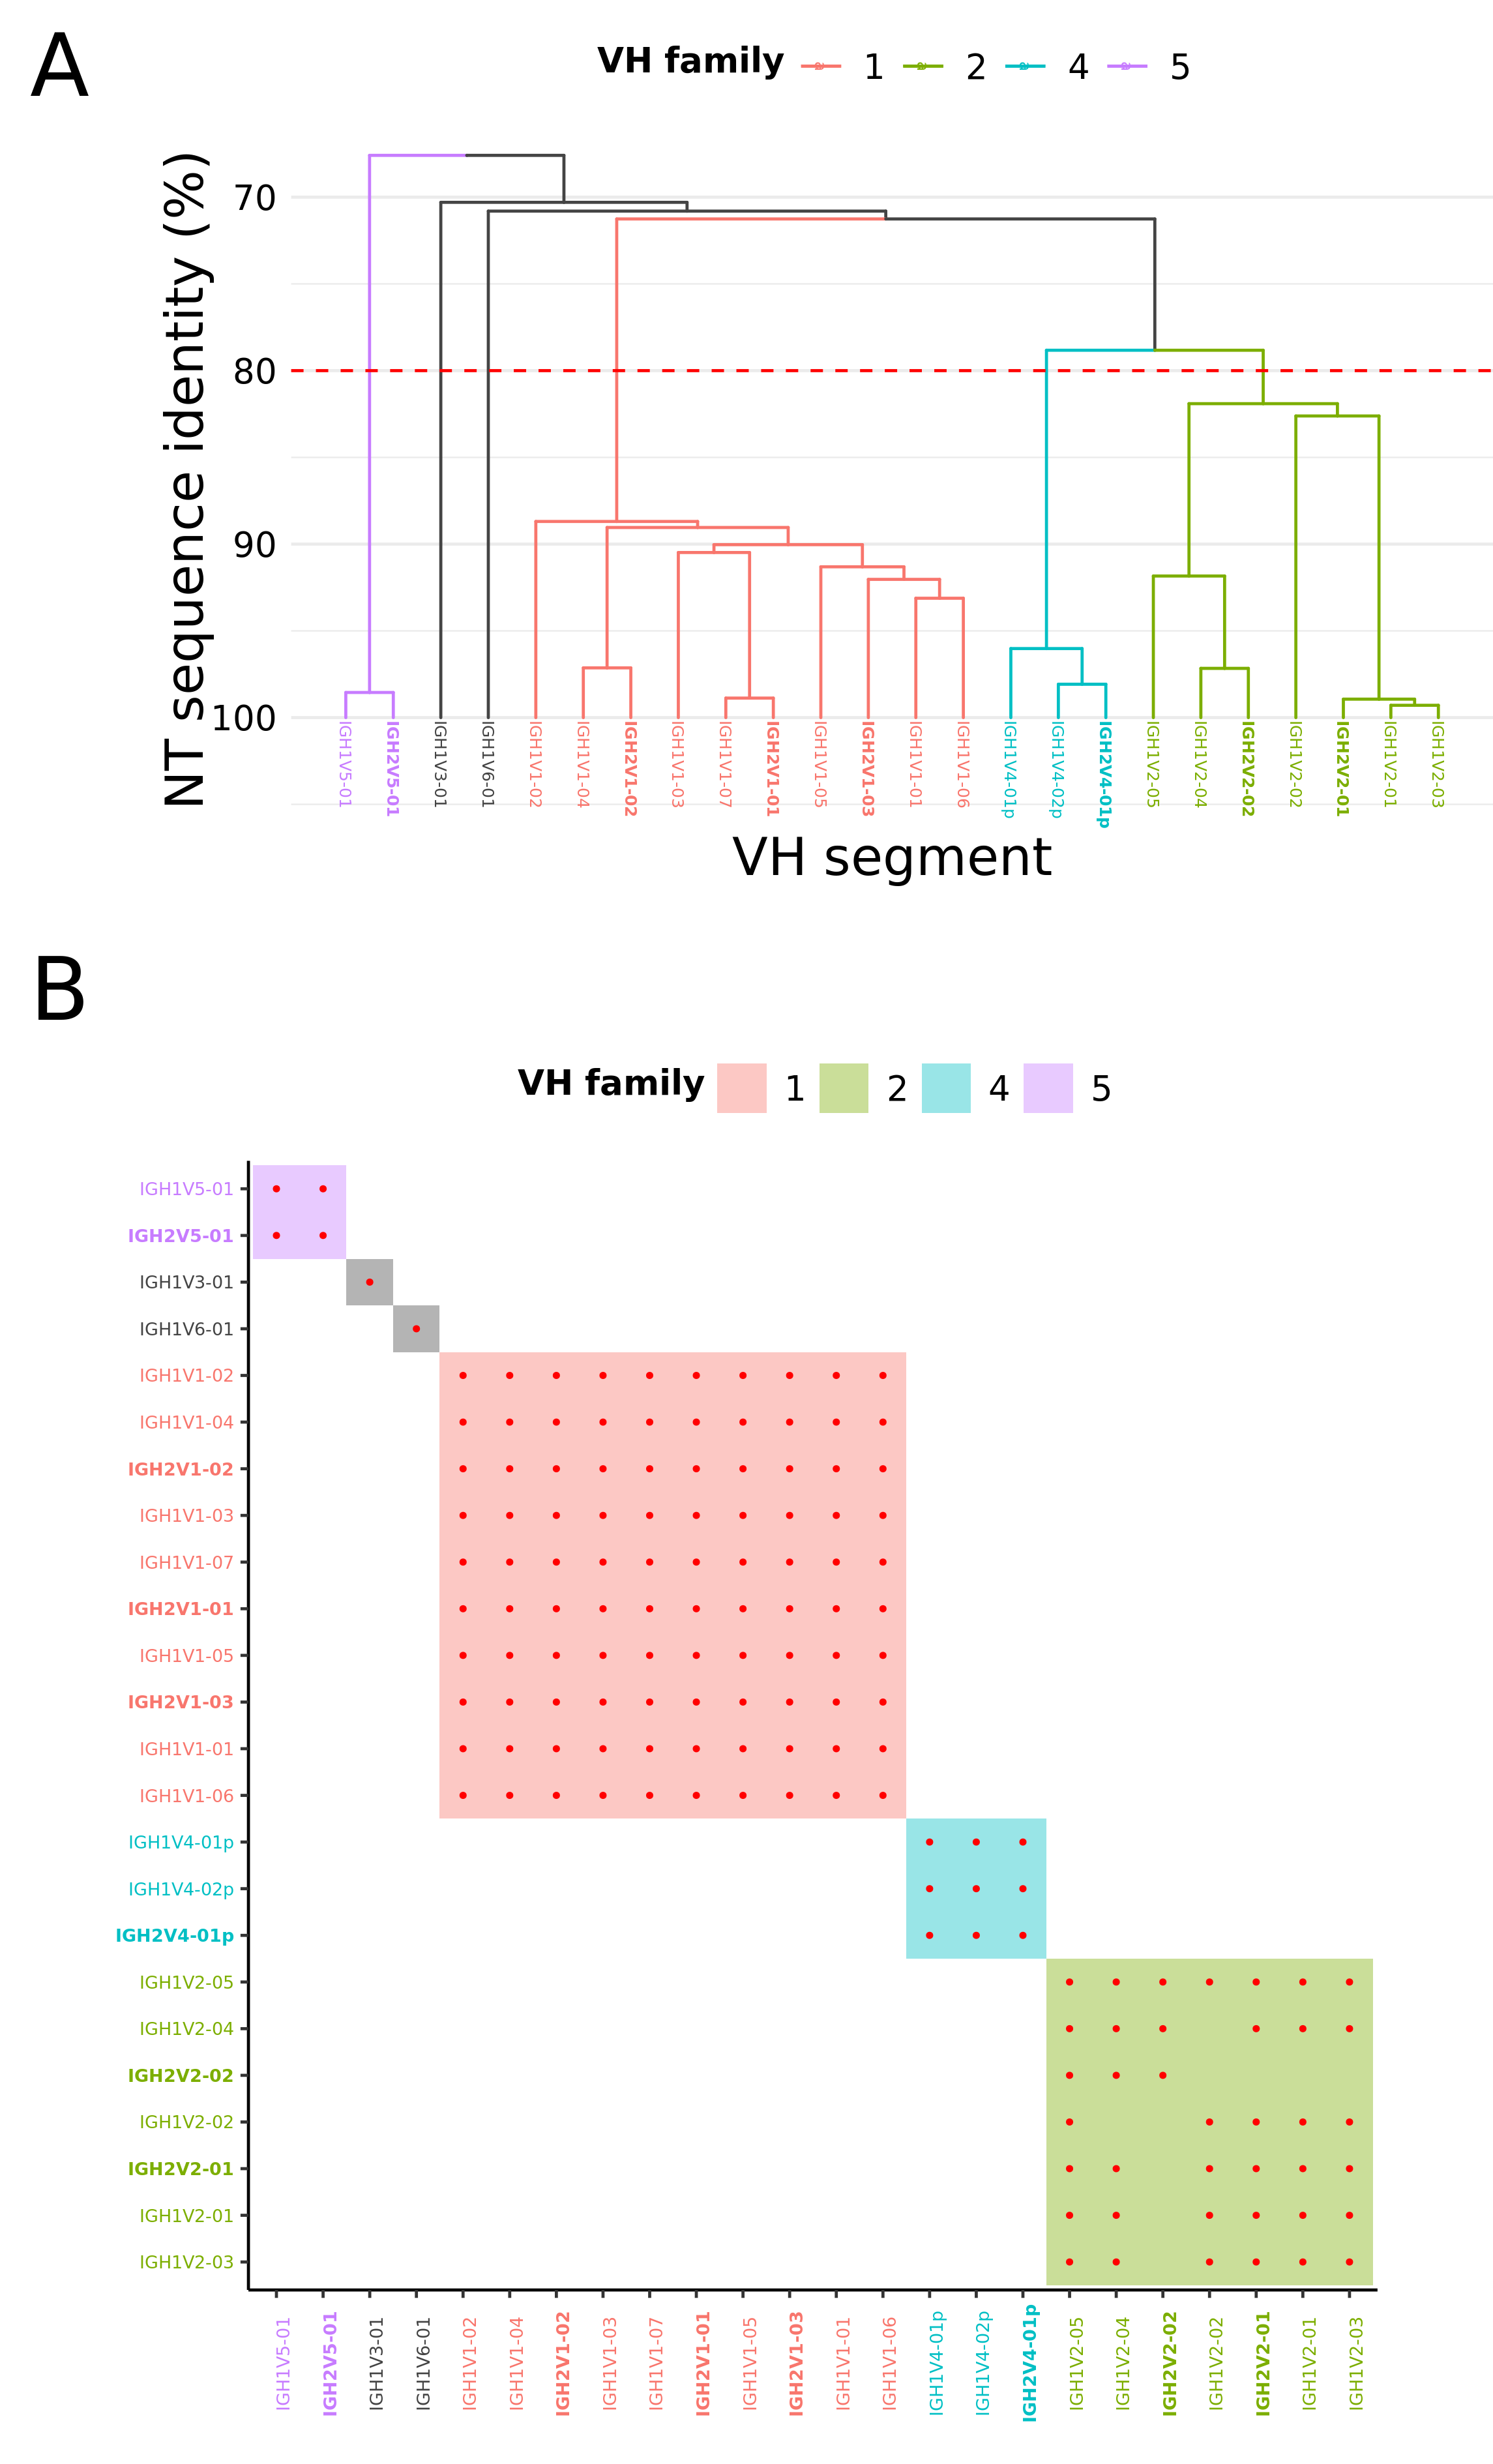
\includegraphics[width=0.8\textwidth]{_Figures/png/nfu-vh-families.png}
	\caption[\vh families in the in \Nfu \textit{IgH} locus]{\textbf{\vh families in the in \Nfu (\textit{IgH}) locus:} (A) Dendrogram of sequence similarity of \vh segments in the \Nfu locus, arranged by single-linkage clustering on nucleotide sequence identity. The red line indicates the 80\% cutoff point for family assignment, while branch colour indicates family membership. (B) Heatmap of family relationships among \Nfu \vh segments, with coloured shading indicating families and red dots indicating pairwise nucleotide sequence identity of at least 80\%. In both subfigures, \vh families containing multiple segments are coloured, single-segment families are in grey, and segments from the IGH2 sublocus are displayed in \textbf{boldface}.}
	\label{fig:nfu-vh-families}
	\end{figure}

	% TODO: Detailed V-co-ordinate table (in appendix)	

\begin{figure}
\centering
	\centering
	\begin{subfigure}{0em}
	\phantomsubcaption{}
    \label{fig:nfu-dj-alignment-a}
    \end{subfigure}
    \begin{subfigure}{0em}
    \phantomsubcaption{}
    \label{fig:nfu-dj-alignment-b}
    \end{subfigure}

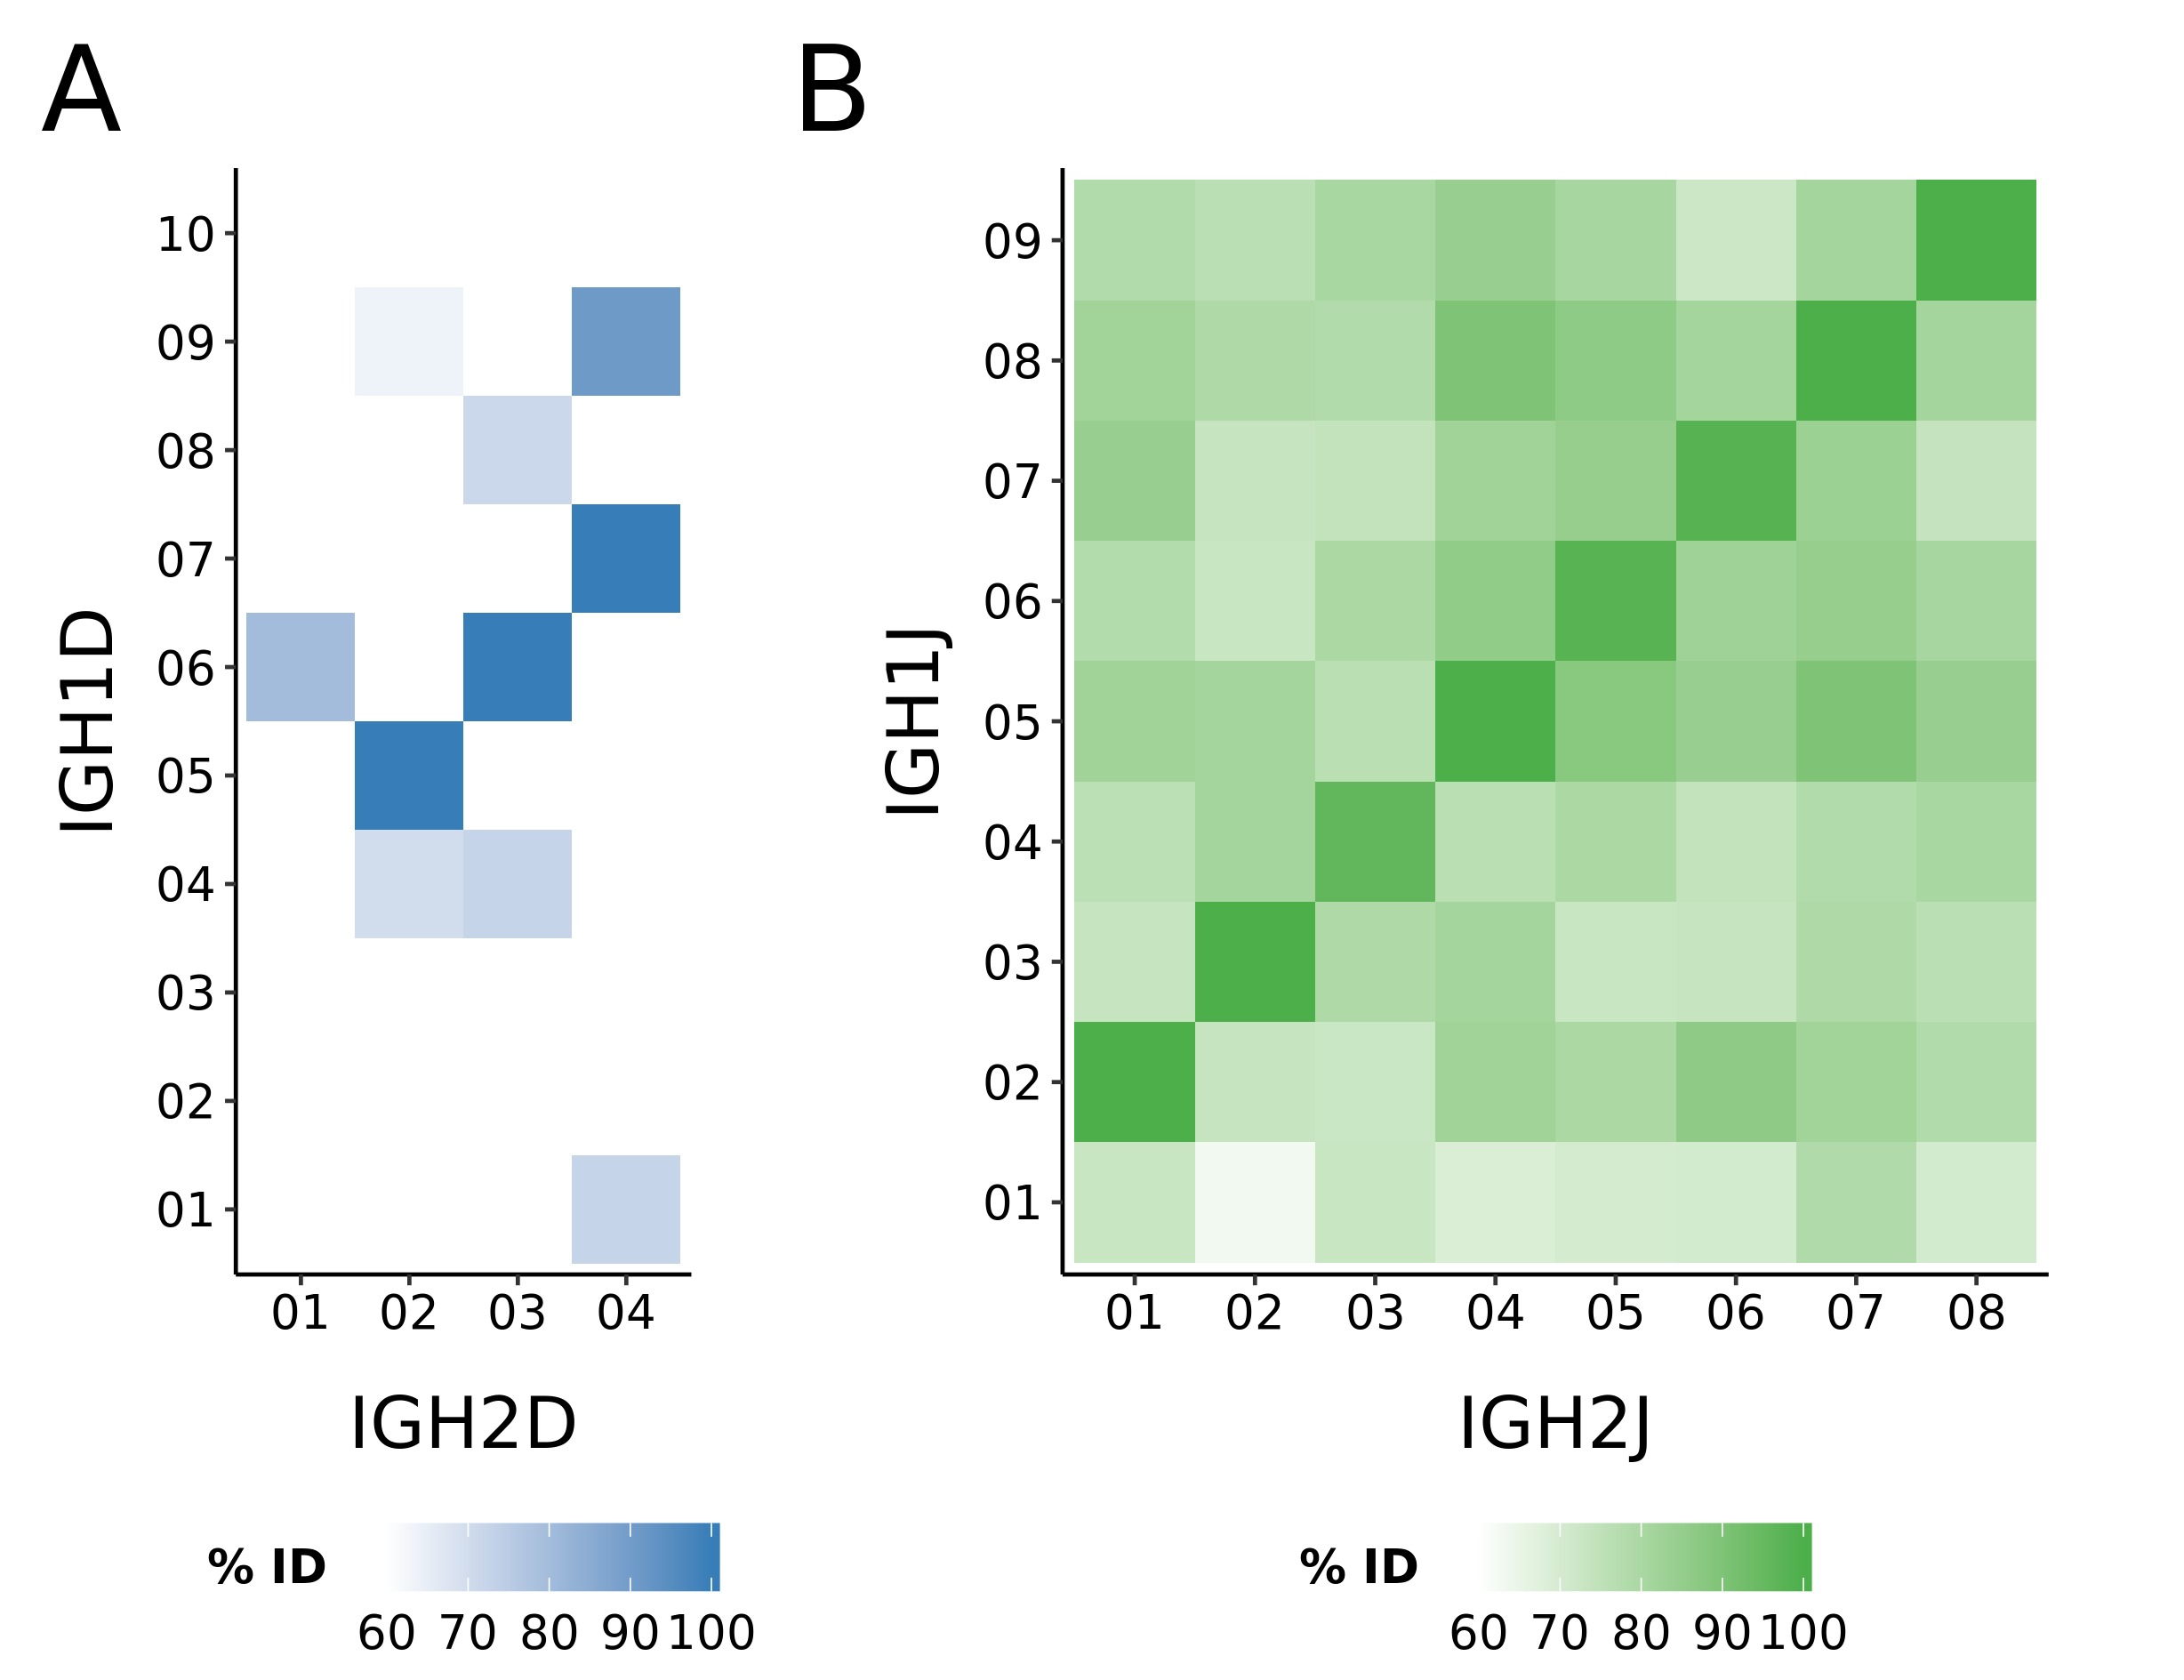
\includegraphics[width=0.6\textwidth]{_Figures/png/nfu-dj-aln}
\caption[Cross-sublocus sequence similarity in \dh and \jh gene segments in \Nfu]{\textbf{Cross-sublocus sequence similarity in \dh and \jh gene segments in \Nfu:} Heatmap of percentage nucleotide sequence identities of Needleman-Wunsch global alignments between (A) \dh and (B) \jh gene segments in IGH1 vs IGH2, revealing syntenic runs of highly similar sequences across both subloci.}
\label{fig:nfu-dj-alignment}
\end{figure}

	\subsubsection{Recombination signal sequences}
	
	In their heptamer sequences, nonamer sequences, and spacer lengths, the recombination signal sequences (RSS) marking the ends of the \vh, \dh and \jh gene segments in the \Nfu locus strongly resemble those of other characterised teleosts, which in turn match those of non-teleost loci (\Cref{fig:nfu-rss-seqlogo-all}). The overall heptamer and nonamer consensus sequences (\texttt{CACAGTG} for heptamers and \texttt{ACAAAAACC} for nonamers) closely matched those expected from the literature, while in 88\% of cases the spacer region was within 1bp of the expected length (12bp for D-RSSs, 23bp for V- and J-RSSs); unexpectedly, the greatest number of \vh-RSSs had a 22bp (rather than 23bp) spacer, but this is not expected to interfere with RSS functionality. Overall, the RSSs in the turquoise killifish appear to be supporting the normal operation of VDJ-recombination in this species.
	
	\begin{figure}
	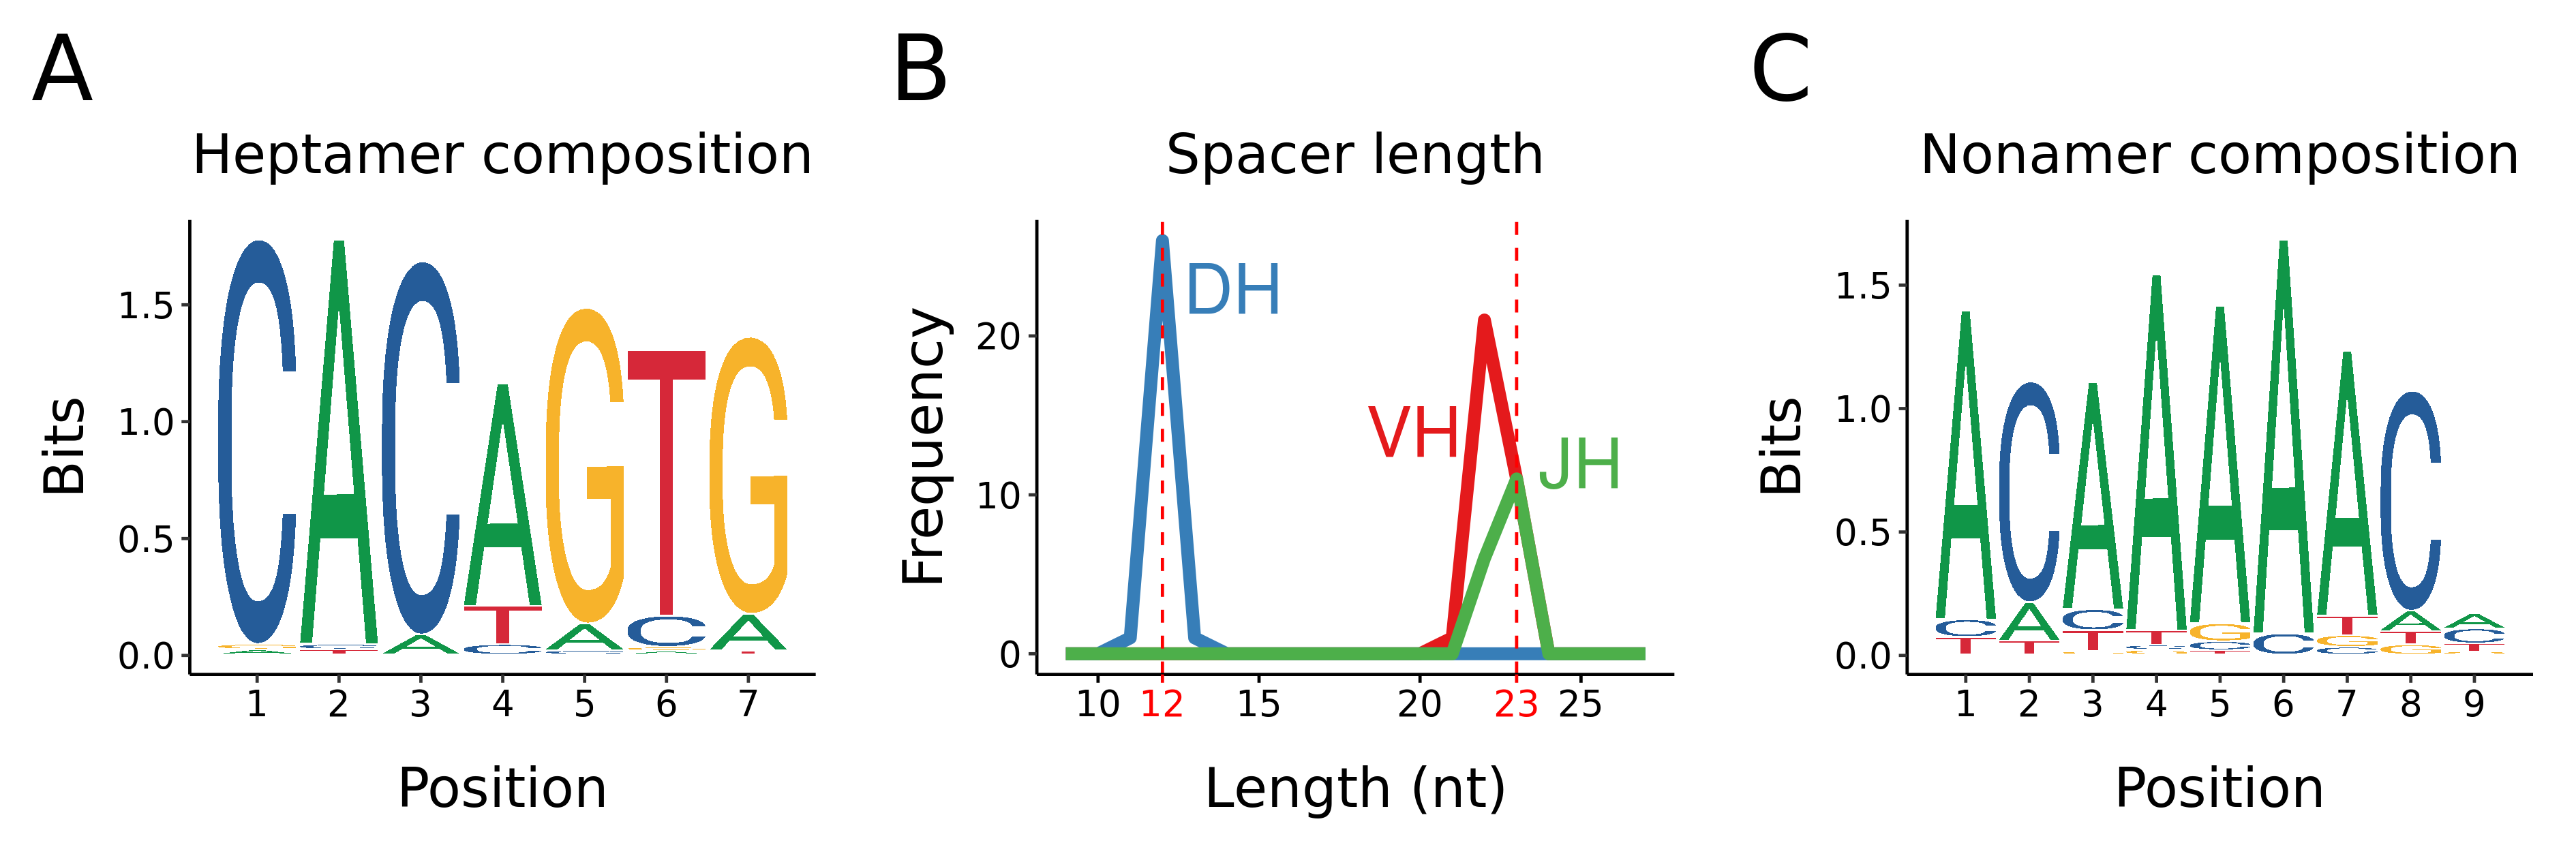
\includegraphics[width=\textwidth]{_Figures/png/nfu-rss-seqlogo-all}
	\caption[Recombination signal sequences in the \Nfu \textit{IGH} locus]{\textbf{Recombination signal sequences in the \Nfu \textit{IGH} locus:} (A) Sequence composition of conserved heptamer sequences across all \Nfu heavy-chain RSSs; (B) length distribution of unconserved spacer sequences in \Nfu heavy-chain RSSs; (C) sequence composition of conserved heptamer sequences across all \Nfu heavy-chain RSSs.}
	\label{fig:nfu-rss-seqlogo-all}
	\end{figure} % TODO: Add in row showing expected consensus sequence with highlighted conserved positions
	
	
	% TODO: Killifish V/D/J RSS sequence logos (separately, in appendix)



	
	\subsection{Discussion}
	
	The turquoise killifish IGH locus shares many features with other characterised teleost loci, including a modified tandem-translocon configuration with intact V, D, J and constant regions (\Cref{fig:nfu-locus-map-b}), four-exon secreted configuration of immunoglobulin M (\Cref{fig:nfu-locus-sashimi-a}), expanded IgD constant region with tandem \cd{}-exon block repeats (\Cref{fig:nfu-locus-sashimi-b,fig:nfu-locus-map-b},), a conserved RSS structure (\Cref{fig:nfu-rss-seqlogo-all}), and a chimeric \cm{1} in IGHD \Cref{fig:nfu-locus-sashimi-b}). However, it also exhibits many ideosyncratic features that differ from those observed in most characterised teleost loci, including an unusually small number of \vh segments (\Cref{fig:nfu-vh-families} and \Cref{tab:teleost-vh-counts}), a four-exon \cm{1}-\cm{2}-TM1-TM2 configuration of transmembrane IgM (\Cref{fig:nfu-locus-sashimi-a}), an inverted sublocus present in antisense (\Cref{fig:nfu-locus-map-b}), and a complete absence of immunoglobulin Z.
	
	Many of these peculiarities, including the unusual IgM-TM splicing pattern, inverted sublocus, and lack of IgZ, are shared with the sublocus of medaka (\textit{Oryzias latipes}), which is the closest relative of \textit{Nothobranchius furzeri} to have its immunoglobulin heavy chain locus characterised prior to this work. Given this close relationship between turquoise killifish and medaka, an obvious hypothesis for the evolutionary history of these unusual traits was of a common origin in the common ancestor of the Cyprinodontiformes (the clade that contains the killifishes) and the Beloniformes (the clade that contains medaka). % Tree for this 

	To investigate this hypothesis further, I performed a complete characterisation of the \textit{IgH} locus in the platyfish \textit{Xiphophorus maculatus} (\Cref{sec:xma-locus}), another cyprinodontiform species that has seen widespread use as a model organism. Alongside this, I performed a more limited characterisation of the \textit{IgH} constant regions in 9 %?
	additional cyprinodontiform and beloniform species, to assess the broader patterns of immunoglobulin heavy chain evolution within these groups (\Cref{sec:comparative-loci}). The results of these additional investigations repeatedly called into question the hypothesis of homology in IgH locus ideosyncracies between medaka and turquoise killifish, and suggest a model of rapid locus evolution within this diverse and important teleost clade.
	
	% TODO: Relationship between killifish Vs and other species
	% TODO: Evolution of IGH1 vs 2
	% TODO: Discussion of mucosal immunity in absence of IGZ
		% TODO: Discuss smallness of killifish locus in the context of relaxed purifying selection and short life span
	% TODO: Section on "Investigating the evolutionary relationship between IGH1 and IGH2"
	% Keep for discussion:
%\q{Given the lack of IgZ in this species, how do you think they carry out mucosal immunity?}
%
%I'd assume using IgM. It's the primitive antibody and is expressed in secreted form in the killifish gut. I haven't investigated the protein expression so it's hard to say for sure, but I'd guess that's the answer. It's also quite possible, lacking a specialised mucosal class, that the answer is ``not very well". It would be very interesting to compare mucosal immune function in species with and without IgZ, especially if those species are closely related.
%
%Given the impressive results indicating the specificity of IgT for mucosal immunity in trout, and the lack of mucosal response of IgM in that species, it would be very interesting to see what mucosal responses look like in a species that lacks that isotype -- is IgM much more responsive and expressed in the gut than in IgT-possessing species, or is the mucosal response just worse?
	% (Incidentally, it would be great to see whether any B-cells in TK show recombinations in both subloci, vs one or the other. Single-cell DNA sequencing could plausibly do this.)



\section{The \textit{IgH} locus in \textit{Xiphophorus maculatus}}
\label{sec:xma-locus}

	\subsection{Overall structure}
	
	The \Xma \textit{IGH} locus occupies roughly 263 kb on chromosome 16 (\Cref{fig:xma-locus-map-a}), in a region syntenic with the part of \textit{Nothobranchius furzeri} chromosome 6 containing the turquoise-killifish IGH locus (\Cref{fig:nfu-xma-igh-synteny}).
	Unlike in \Nfu, and medaka, only a single ``sublocus" is present, which spans the entire length of the locus region; no evidence of a second, antisense locus could be identified. The overall structure of this locus roughly corresponds to that of simpler that of simpler teleost loci like those of zebrafish and fugu, albeit with some striking ideosyncracies, and it differs from that of \Nfu in several important respects.
	
	\begin{figure}
	\centering
	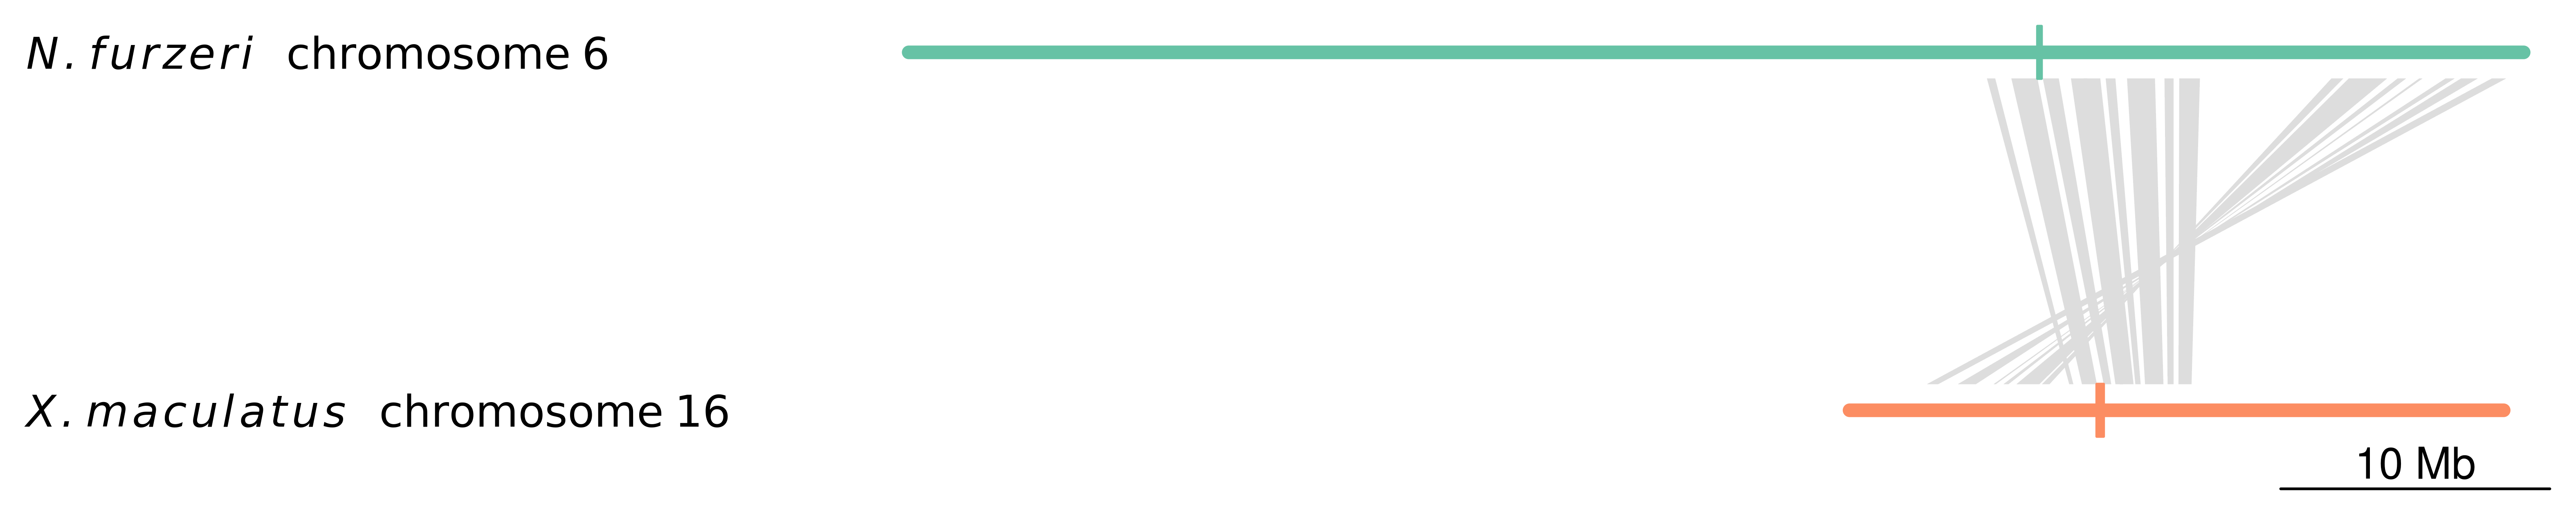
\includegraphics[width=\textwidth]{_Figures/png/nfu-xma-igh-synteny}
	\caption[Synteny between \textit{IGH}-bearing chromosomes of \Nfu and \Xma]{\textbf{Synteny between \textit{IGH}-bearing chromosomes of \Nfu and \Xma:} Plot of syntenic regions from \Nfu chromosome 6 and \Xma chromosome 16, showing syntenic regions (light grey) and \textit{IGH} loci (coloured rectangles). While not syntenic themselves, the \textit{IGH} loci of both species are immediately flanked by matching syntenic regions on both sides. Synteny data provided by Willemsen \textit{et al.} (\dots)} % TODO: Credit David's/Ray's paper
	\label{fig:nfu-xma-igh-synteny}
	\end{figure}
	
	\begin{figure}
	\centering
	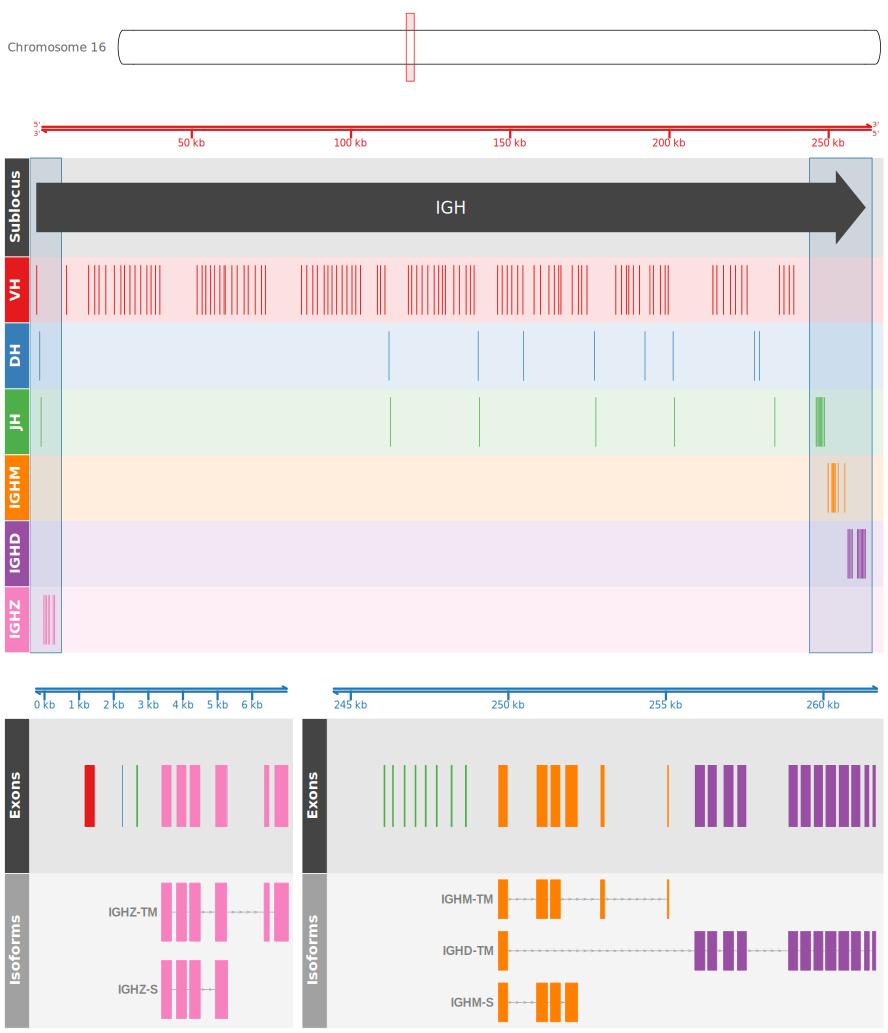
\includegraphics[width=\textwidth]{/home/will/Documents/code/figures/2018-11-07/xma-locus-map}
	\caption[The immunoglobulin heavy chain (\textit{IGH}) locus in \textit{}]{\textbf{The immunoglobulin heavy chain (\textit{IGH}) locus in \textit{Xiphophorus maculatus}:} (A) Position of the \textit{IGH} locus on chromosome (group) 16 of the \Xma genome. (B) Arrangement of \vh, \dh, \jh and constant-region gene segments on the \Xma \textit{IgH} locus. (C) Detailed map of the \textit{IGHZ} and \textit{IGHM/D} constant regions, indicating the position and identity of the constant-region exons and the exon composition of expressed \textit{IgH} isoforms in \Xma.}
	\begin{subfigure}{0em}
        \phantomsubcaption{}
        \label{fig:xma-locus-map-a}
    \end{subfigure}
    \begin{subfigure}{0em}
        \phantomsubcaption{}
        \label{fig:xma-locus-map-b}
    \end{subfigure}
    \begin{subfigure}{0em}
        \phantomsubcaption{}
        \label{fig:xma-locus-map-c}
    \end{subfigure}
	\label{fig:xma-locus-map}
\end{figure}

	
	\subsection{Constant regions}
	
	Most strikingly, unlike the turquoise killifish, the platyfish locus contains a fully intact IGHZ constant region, with a six-exon structure homologous with that seen in most other teleost loci (unlike in stickleback, the exon corresponding to \cz{2} is not missing) and a secretory tail produced by a run-on event from \cm{4} (\Cref{fig:xma-locus-map-b,fig:xma-locus-map-c}). Conversely, the genomic configurations of the IGHM and IGHD constant regions were highly similar to those of turquoise killifish, with a {\cm{1}-\cm{2}-\cm{3}-\cm{4}-TM1-TM2} configuration for IGHM and a {\cd{1}-(\cd{2}-\cd{3}-\cd{4})$_2$-\cd{5}-\cd{6}-\cd{7}-TM1-TM2} configuration for IGHD. The evolution of constant-region exon structure in the cyprinodontiforms, including the pattern of (\cd{2}-\cd{3}-\cd{4}) duplications, is discussed more in \dots .
	
	In order to investigate the expressed isoforms present in \Xma, published RNA-sequencing reads from platyfish \dots % Tissues used, reference
	were aligned to the IGHZ and IGHM/D constant regions with STAR. % TODO: Refer to methods here
	The results indicate the expected splice patterns for IGHZ and IGHD, including a six-exon configuration for IGHZ-TM (\Cref{fig:xma-locus-sashimi-z}), the use of a \bp{23} secretory tail produced by a run-on event from \cz{4} in IGHZ-S, and the presence of a chimeric \cm{1} exon in IGHD-TM (\Cref{fig:xma-locus-sashimi-d}). However, while secretory IGHM (IGHM-S) in platyfish was found to occupy the expected four-exon configuration seen in turquoise killifish and elsewhere (\Cref{fig:xma-locus-sashimi-m}), the configuration observed for transmembrane IGHM (IGHM-TM) did not correspond to the four-exon structure shared between turquoise killifish and medaka (\Cref{fig:nfu-locus-sashimi-a}). Rather, IGHM-TM in \Xma occupies the standard five-exon configuration seen in most characterised teleosts (\Cref{fig:teleost-igm-exons-d}). This surprising difference raises not only the question of the evolutionary history of this ideosyncratic splicing configuration, but also that of what, if any, functional difference arises from the presence or absence of \cm{3} in transmembrane IgM in different species. % TODO: Discuss possible experiments?

	The examination of the constant-region structures present in the \Xma IGH locus therefore reveals three notable features that differ in state between medaka, turquoise killifish, and the southern platyfish. Most strikingly, the absence of IGHM in medaka and killifish, but its presence in platyfish, strongly suggests that the isoform has been lost independently in the two groups. Conversely, the presence of a four-exon IGHM-TM in medaka and killifish, but a five-exon configuration in platyfish, is less clear-cut: it may indicate an independent change in medaka and killifish that is absent in platyfish, but may also plausibly represent a reversion in platyfish to the more-primitive five-exon state. Without a deeper understanding of the currently-unknown physical underpinnings of this observed difference in splicing behaviour, this question can only be addressed through analysis of RNA-seq data from a large number of related species, something beyond the scope of the present investigation. % TODO: Do it anyway?
	Finally, the presence of a (\cd{2}-\cd{3}-\cd{4}) duplication in both platyfish and killifish, but not in medaka, suggests that this may be a shared primitive feature of the Cyprinodontiforms; however, given the apparent recurrence of this duplication pattern in many different groups across the teleosts, a strong conclusion cannot be drawn without a higher-resolution phylogenetic analysis of a larger number of related species. % TODO: See section ... etc.
	
			\begin{figure}
	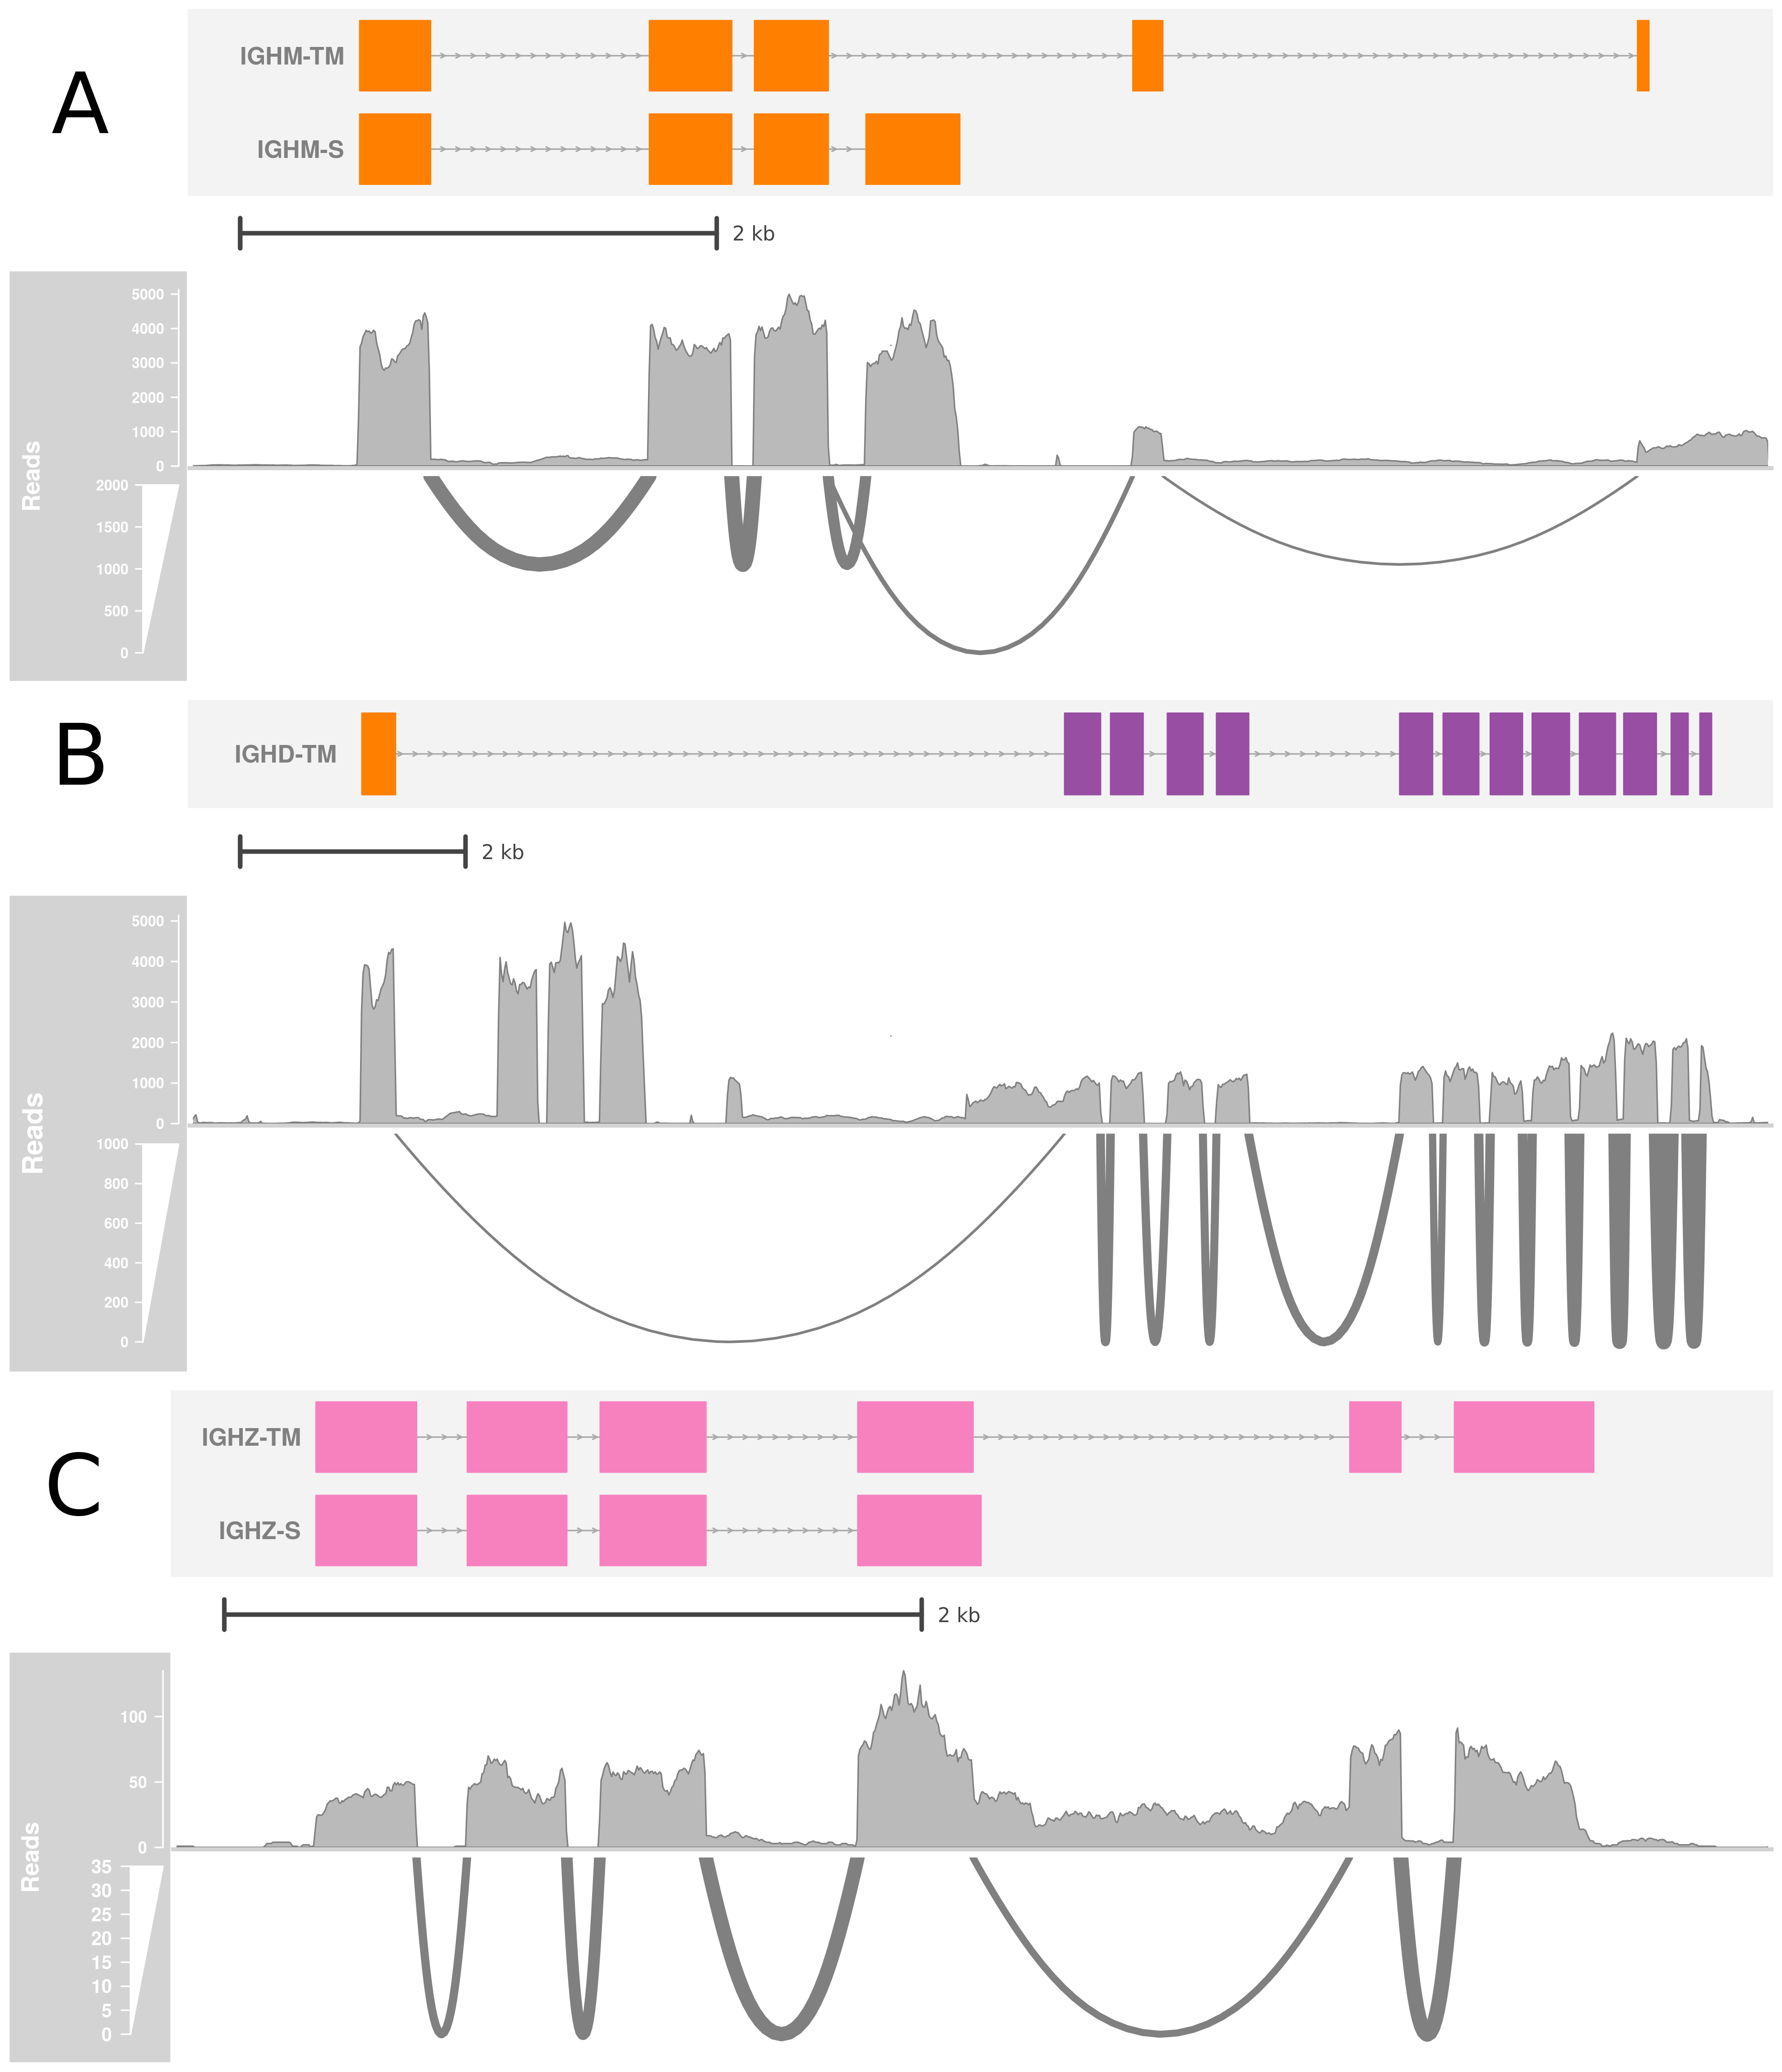
\includegraphics[width=\textwidth]{_Figures/png/xma-locus-sashimi}
	\begin{subfigure}{0em}
        \phantomsubcaption{}
        \label{fig:xma-locus-sashimi-m}
    \end{subfigure}
    \begin{subfigure}{0em}
        \phantomsubcaption{}
        \label{fig:xma-locus-sashimi-d}
    \end{subfigure}
    \begin{subfigure}{0em}
        \phantomsubcaption{}
        \label{fig:xma-locus-sashimi-z}
    \end{subfigure}
	\caption[Constant-region isoforms in \Xma]{\textbf{Constant-region isoforms in \Xma:} Coverage and sashimi plots of STAR-aligned RNA-seq reads from \Xma samples, demonstrating the splicing behaviour of IGH1 constant-region isoforms. (A) IGHM exon splicing, showing alternative splicing patterns of IGHM-TM and IGHM-S; (B) IGHD exon splicing, including splicing of \cm{1} to \cd{1}; (C) IGHZ exon splicing.}
	\label{fig:xma-locus-sashimi}
	\end{figure}

	
	\subsection{Variable regions}
	
	In total, 99 \vh segments, 9 \dh segments and 14 \jh segments were identified in the \Xma IGH locus. In all cases, the great majority of these segments appear to exclusively serve IGHM and IGHD and exclude IGHZ; as in most teleost IGH loci, the IGHZ constant region in \Xma has its own dedicated \dh and \jh regions (IGHDZ01 and IGHJZ01) separate from those serving IGHM and IGHD; % TODO: Compare these to the orphaned D/J segments in TK to test vestigial IGHZ hypothesis
in addition, unlike in most teleost loci, the \Xma IGHZ constant region is upstream of the majority of \vh segments in the locus, with only a single \vh segment between the start of the locus and IGHDZ01. This lone \vh segment, IGHV01-01, is distinct in sequence from the other \vh segments in the locus (\Cref{fig:xma-vh-families-tree,fig:xma-vh-families-map}, second from left), but appears to be functional; its status as the only \vh segment upstream of IGHZ indicates that the potential sequence diversity available to this isotype is very limited, with only a single VDJ combination available to the recombination process. In this case, any and all antigen-binding diversity in \textit{Xiphophorus} \textit{IGHZ} must arise from junctional diversity alone. 

	Unlike the IGHZ variable region, the \vh region downstream of IGHZ but upstream of IGHM is highly expanded, with 98 identified \vh segments -- more than four times the total number seen in \Nfu, and almost six times the number in the largest \Nfu sublocus. At least 74 of these \vh segments appear to be fully in-frame and functional and equipped with functional RSS sequences, representing one of the highest numbers of functional \vh segments seen in any teleost IGH locus; it remains to be seen whether IGHV01-01 is also capable of recombining with \dh segments downstream of the IGHZ constant region, and so constitutes part of the range of VDJ combinations available to IGHM and IGHD. The \vh sequences in the \Xma locus are much more tightly packed than in the \Nfu locus, consistent with a lower overall prevalence of repetitive regions (21\%) in the \Xma genome. However, the final four \vh segments (of which two are structurally intact) are downstream of the last identified \dh segment and inverted relative to the rest of the locus, and may not be able to successfully undergo VDJ recombination. 
	
	In total, the \vh regions in \Xma \textit{IGH} fall into 22 families, of which six contain multiple segments; strikingly, the single \vh segment serving IGHZ (IGHV01-01) represents a distinct family which is distinct from any other segment in the locus \Cref{fig:xma-vh-families-tree}. 	There is a clear interrelationship between the \vh families observed in the \Xma locus and those found in the \Nfu locus. The largest families in both loci (\Xma V02 and \Nfu V1) share a clear common ancestor within the \vh tree (\Cref{fig:nfu-xma-vh-tree-nt}), as do the second-largest families (\Xma V03 and \Nfu V2), indicating that these families play a conserved evolutionary role across the cyprinodontiforms. In accordance with the close sequence relationship noted in \Cref{sec:nfu-locus-variable-families}, \Nfu V4 falls comfortably within the V03/V2 subtree, supporting their status as a pseudogenised subfamily of \Nfu V2. 
		
	In addition to its highly expanded \vh region, the variable region of the \Xma locus is unusual in the arrangement of its \dh and (to a lesser extent) its \jh regions. Rather than a single, relatively densely-packed D-region, the \Xma locus contains \dh segments interspersed throughout the long stretch of the locus between the end of the \textit{IGHZ} constant region and the start of that of IGHM. Many of these lone \dh segments are closely associated with single \jh segments, raising the possibility of a more cluster-like behaviour in which each $V_n-D_{1-2}-J_1$ group acts as a distinct recombination unit. However, the presence of a dense eight-segment J-region immediately upstream of IGHM suggests a more conventional translocon behaviour; it remains to be seen which of these traditional models of antigen-receptor structure more closely matches the \textit{in vivo} recombination behaviour of this locus.
	
	% TODO: Discuss here phylogenetic relationship between Nfu and Xma \dh and (esp) \jh segments (esp. eight segments in main \jh block)
	
	Finally, as is the case with \Nfu, the recombination signal sequences (RSSs) in \Xma IGH correspond closely to the standard expectations across the vertebrates, with the expected heptamer and nonamer consensus sequences (\Cref{fig:xma-rss-seqlogo-all-heptamer,fig:xma-rss-seqlogo-all-nonamer}) and spacer length distributions (\Cref{fig:xma-rss-seqlogo-all-spacer}, 95\% of RSS spacers within \bp{1} of the expected conserved length).
	

% TODO: compare \vh families from platy and TK, align C-exons between TK and platy (and other cyprinodontiforms)
	
	
	\begin{figure}
	\centering
	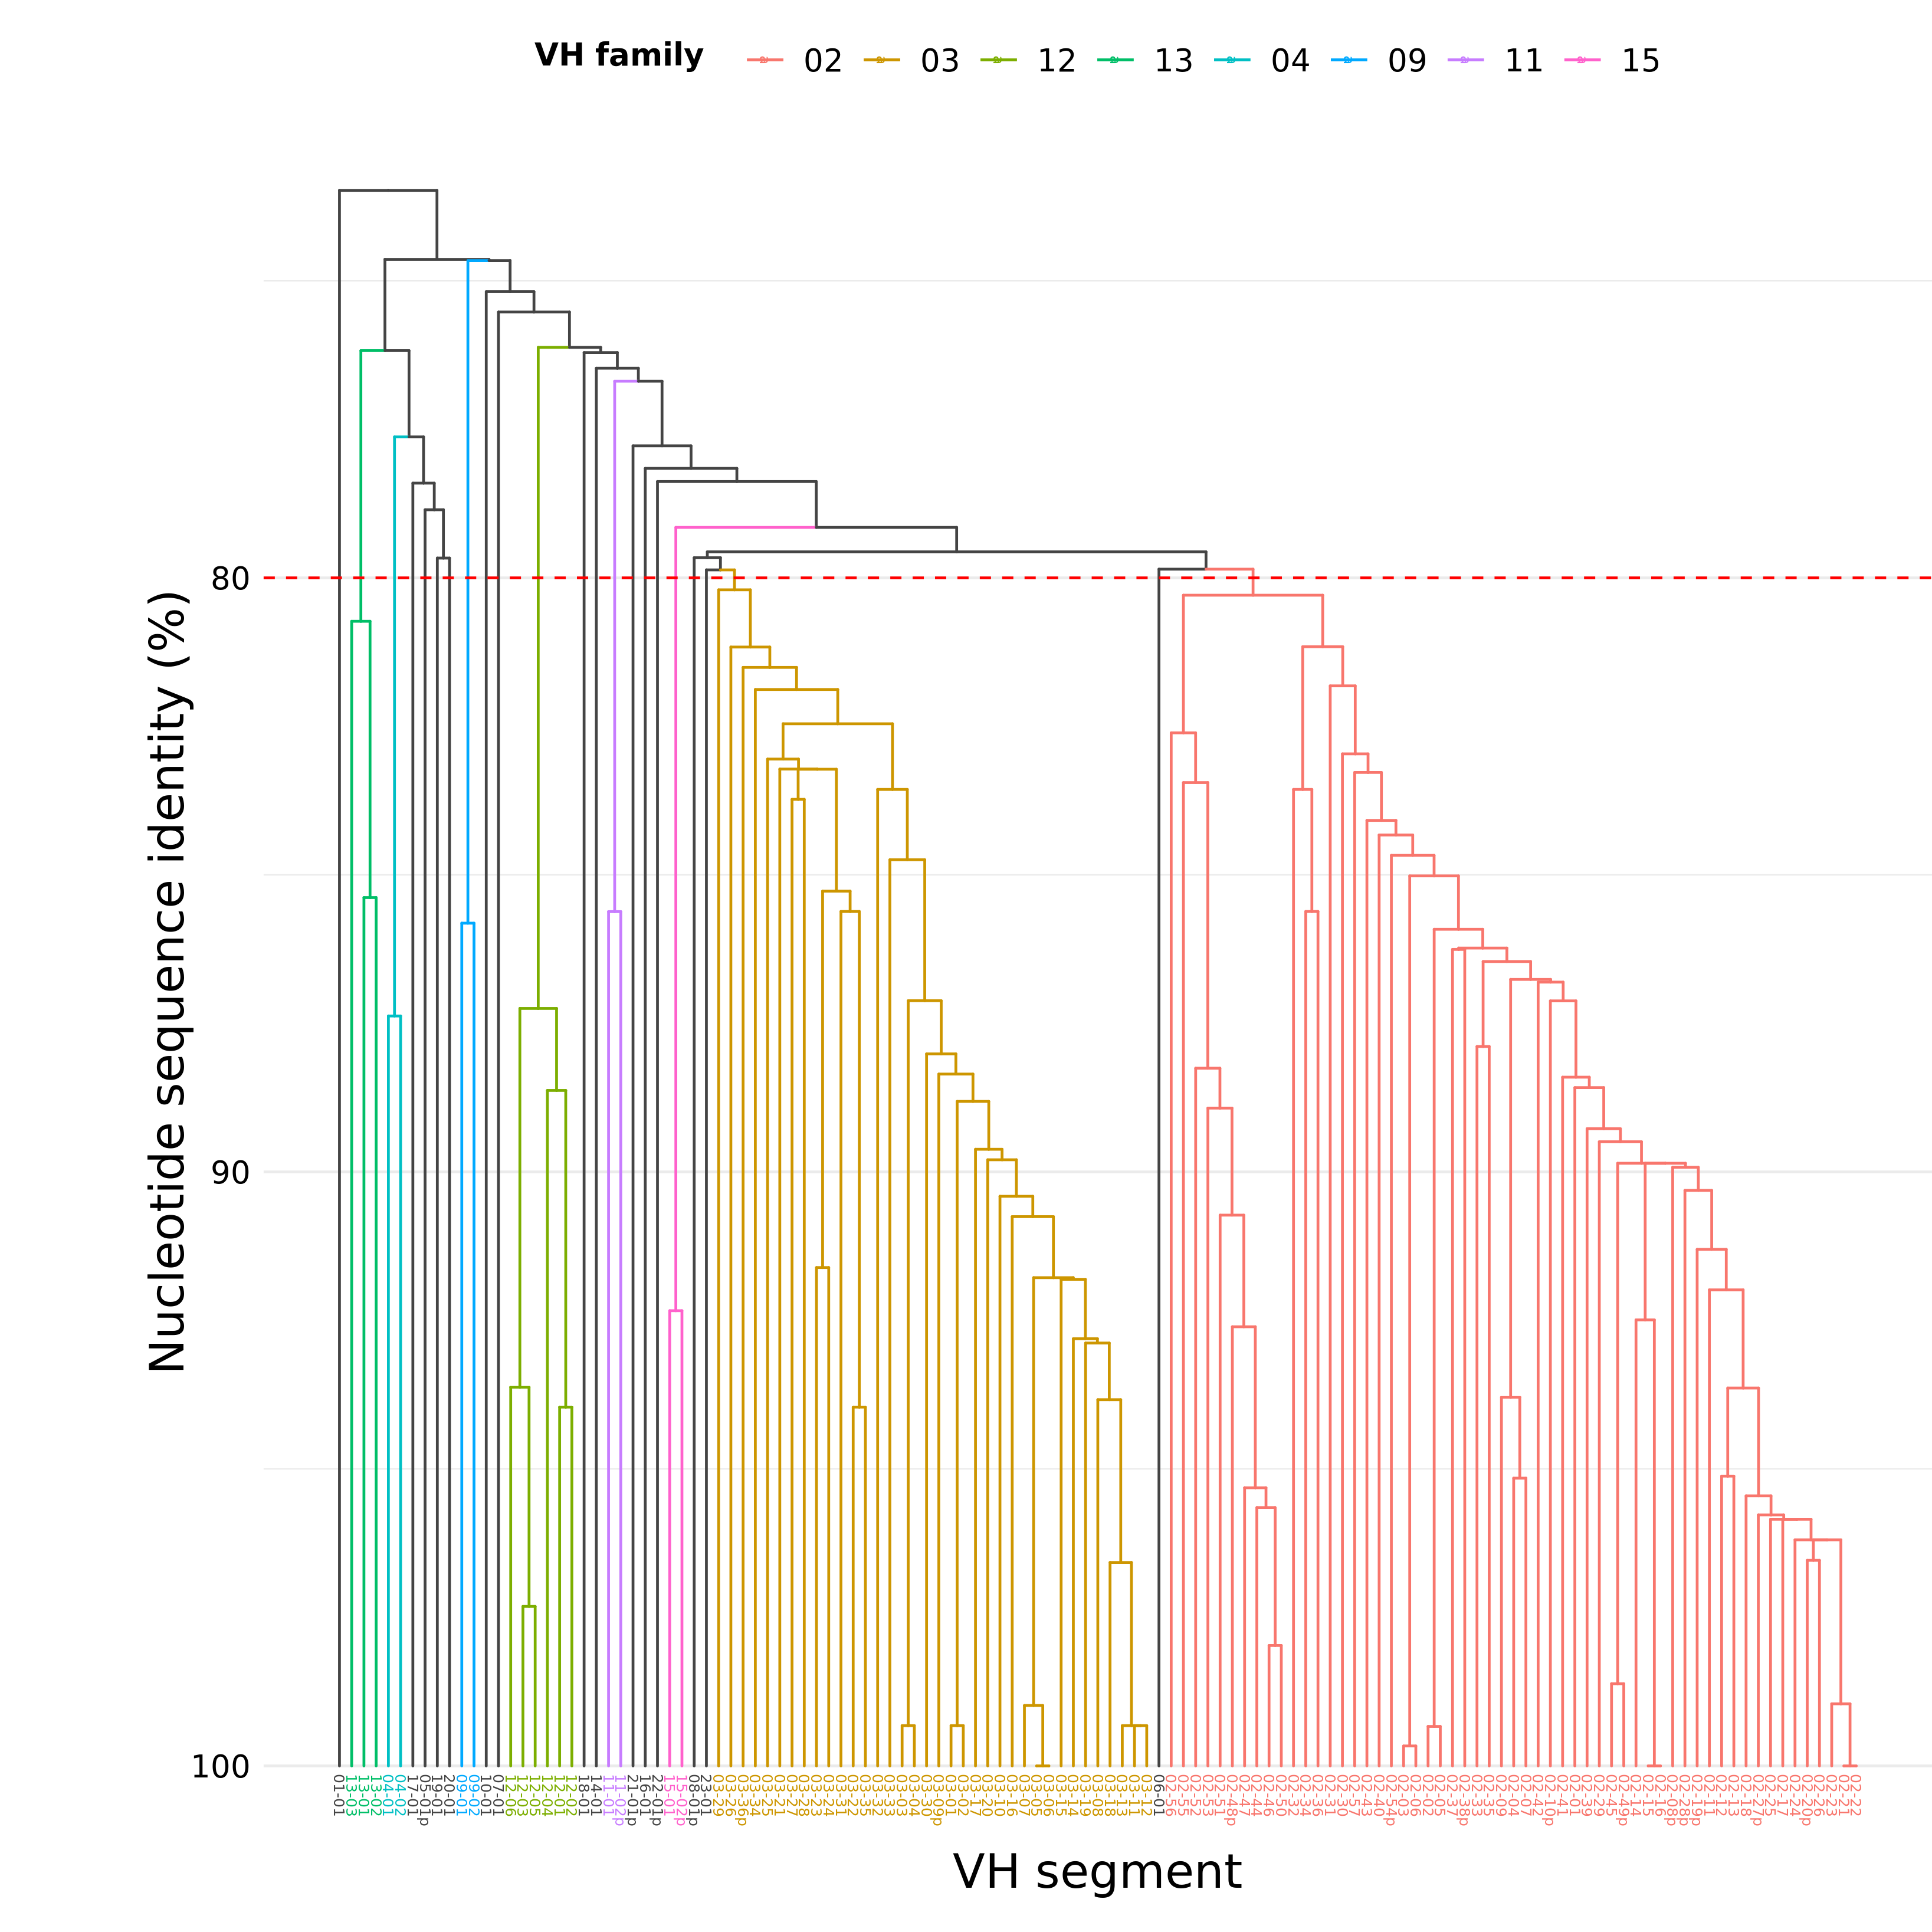
\includegraphics[width=\textwidth]{_Figures/png/xma-vh-families-tree}
	\caption[Dendrogram of \vh families in the in \Xma \textit{IgH} locus]{\textbf{Dendrogram of \vh families in the in \Xma (\textit{IgH}) locus:} Dendrogram of sequence similarity of \vh segments in the \Xma locus, arranged by single-linkage clustering on nucleotide sequence identity. The red line indicates the 80\% cutoff point for family assignment, while branch colour indicates family membership:  \vh families containing multiple segments are uniquely coloured, while single-segment families are in grey.}
	\label{fig:xma-vh-families-tree}
	\end{figure}
	
	\begin{figure}
	\centering
	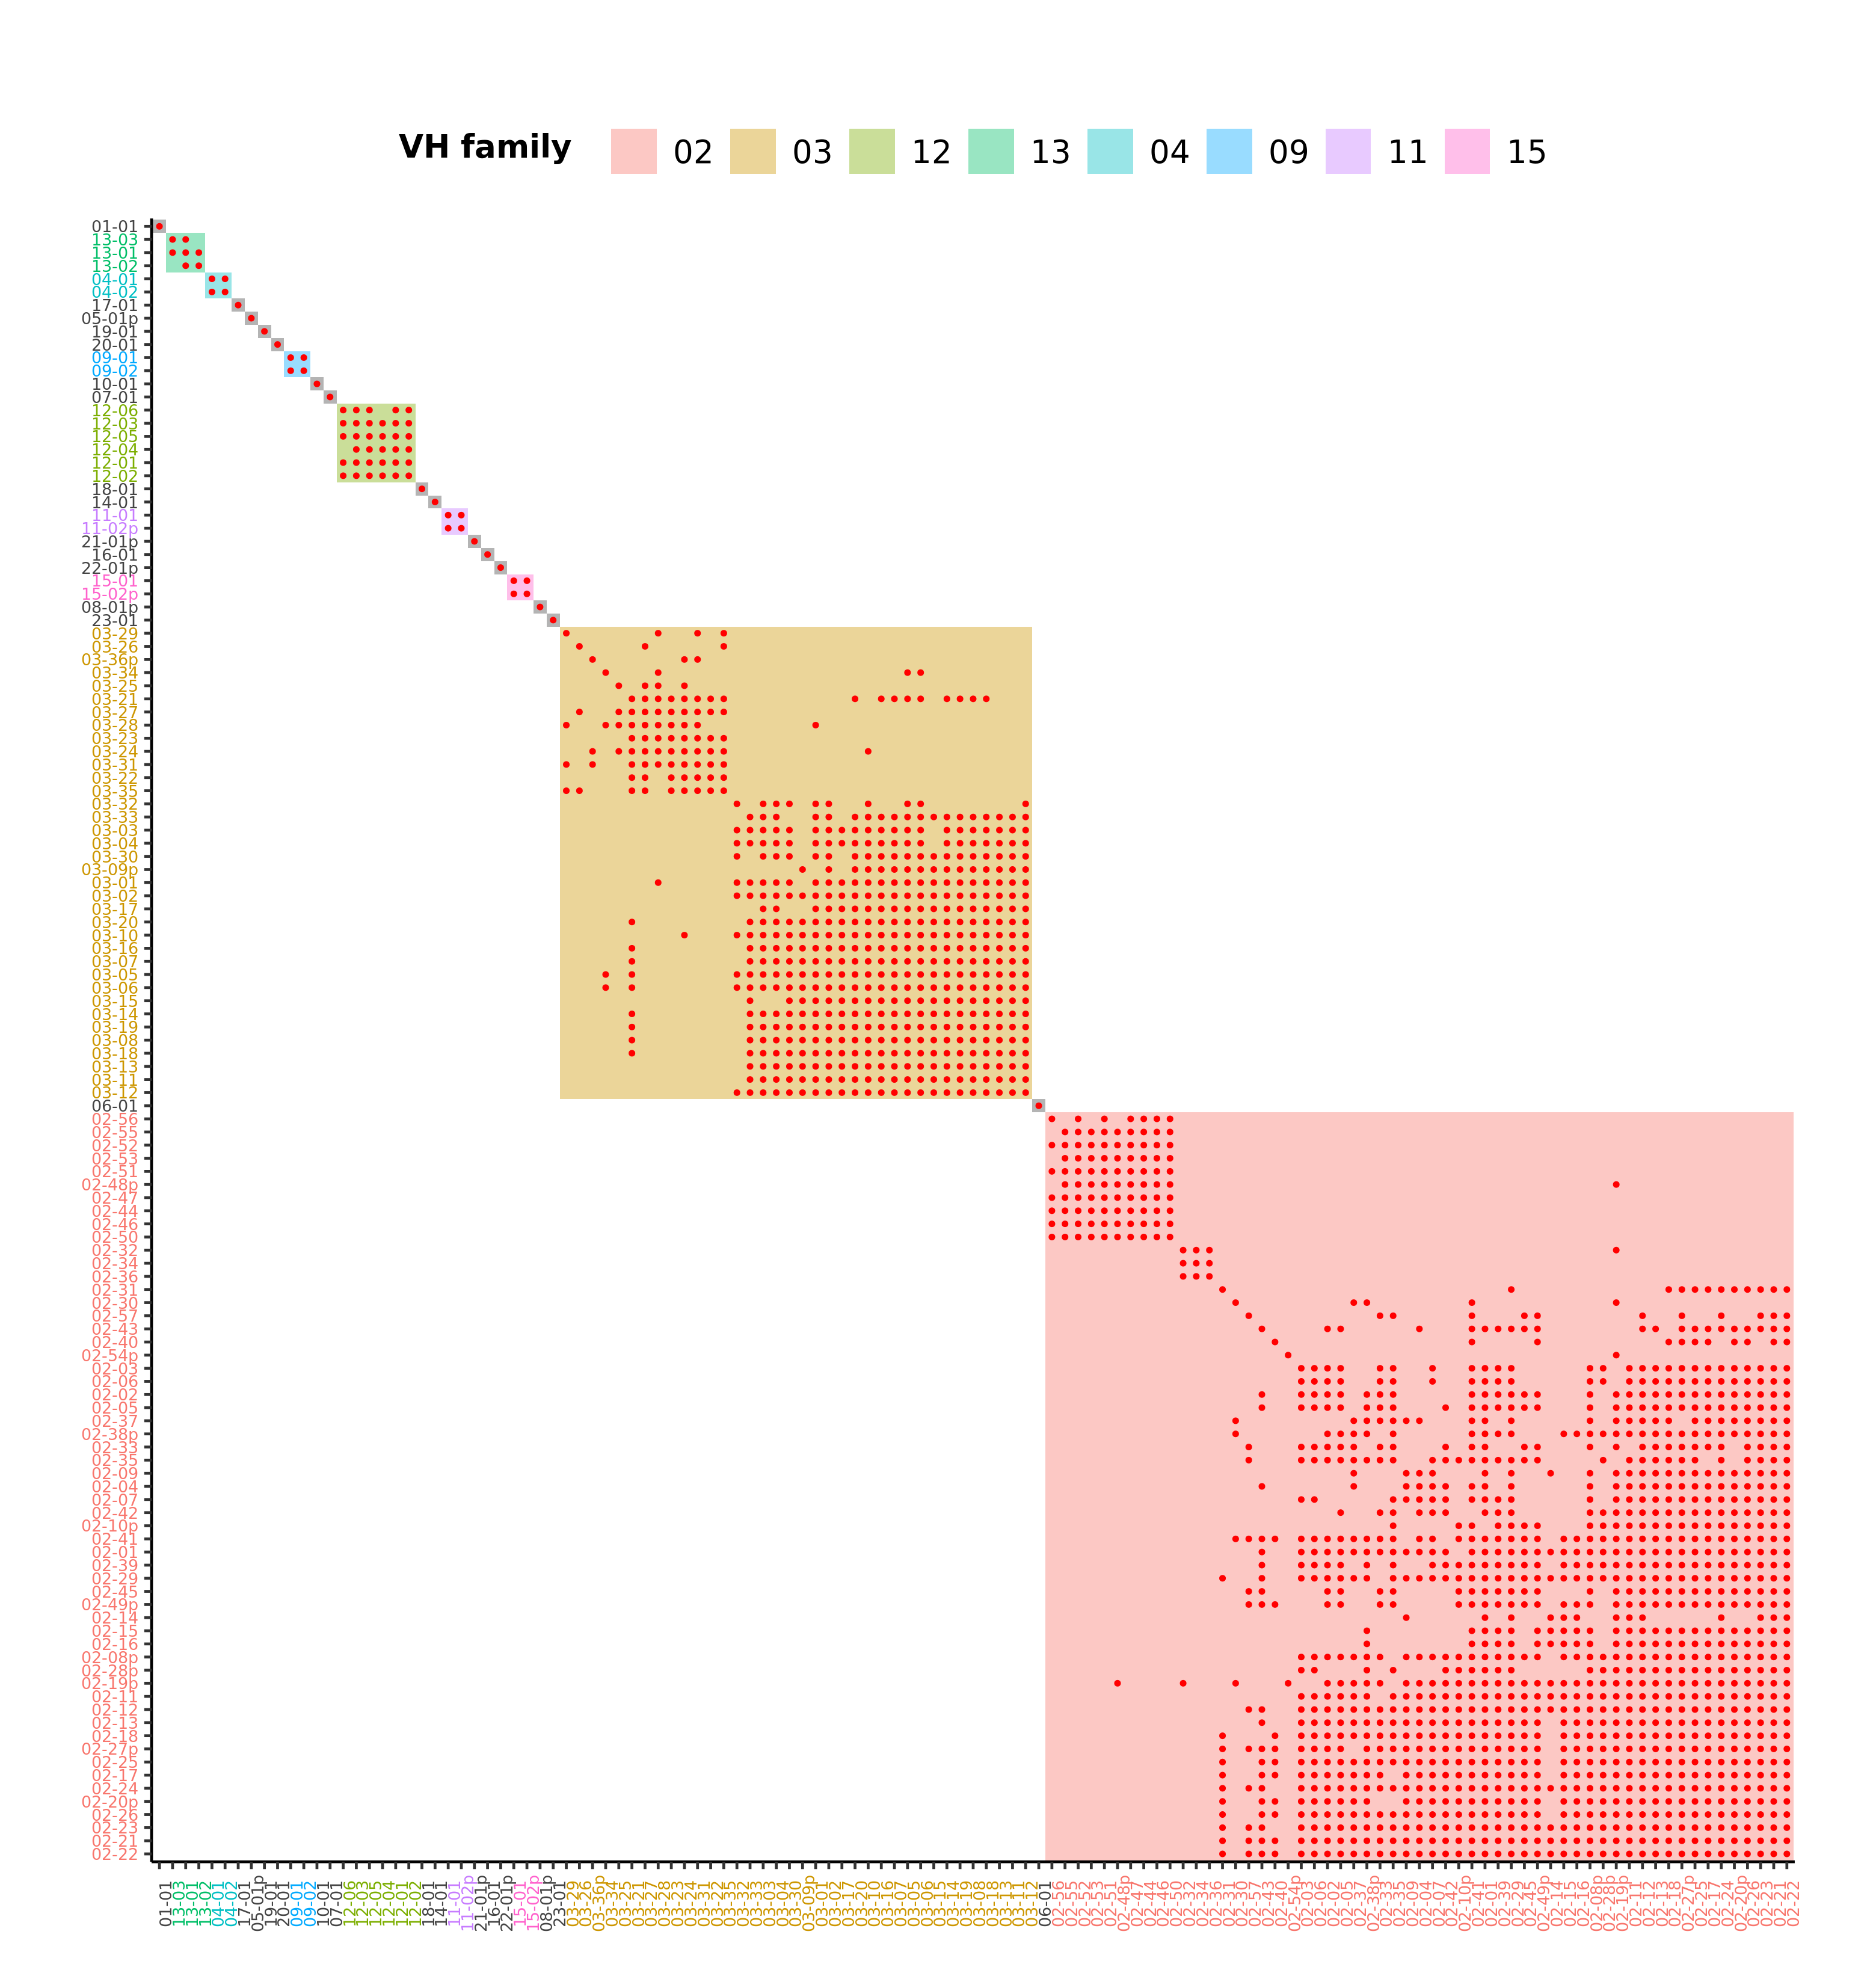
\includegraphics[width=\textwidth]{_Figures/png/xma-vh-families-map}
	\caption[Heatmap of \vh families in the in \Xma \textit{IgH} locus]{\textbf{Heatmap of \vh families in the in \Xma (\textit{IgH}) locus:} Heatmap of family relationships among \Xma \vh segments, with coloured shading indicating families and red dots indicating pairwise nucleotide sequence identity of at least 80\%. \vh families containing multiple segments are uniquely coloured, while single-segment families are in grey.}
	\label{fig:xma-vh-families-map}
	\end{figure}
	
	\begin{figure}
	\centering
	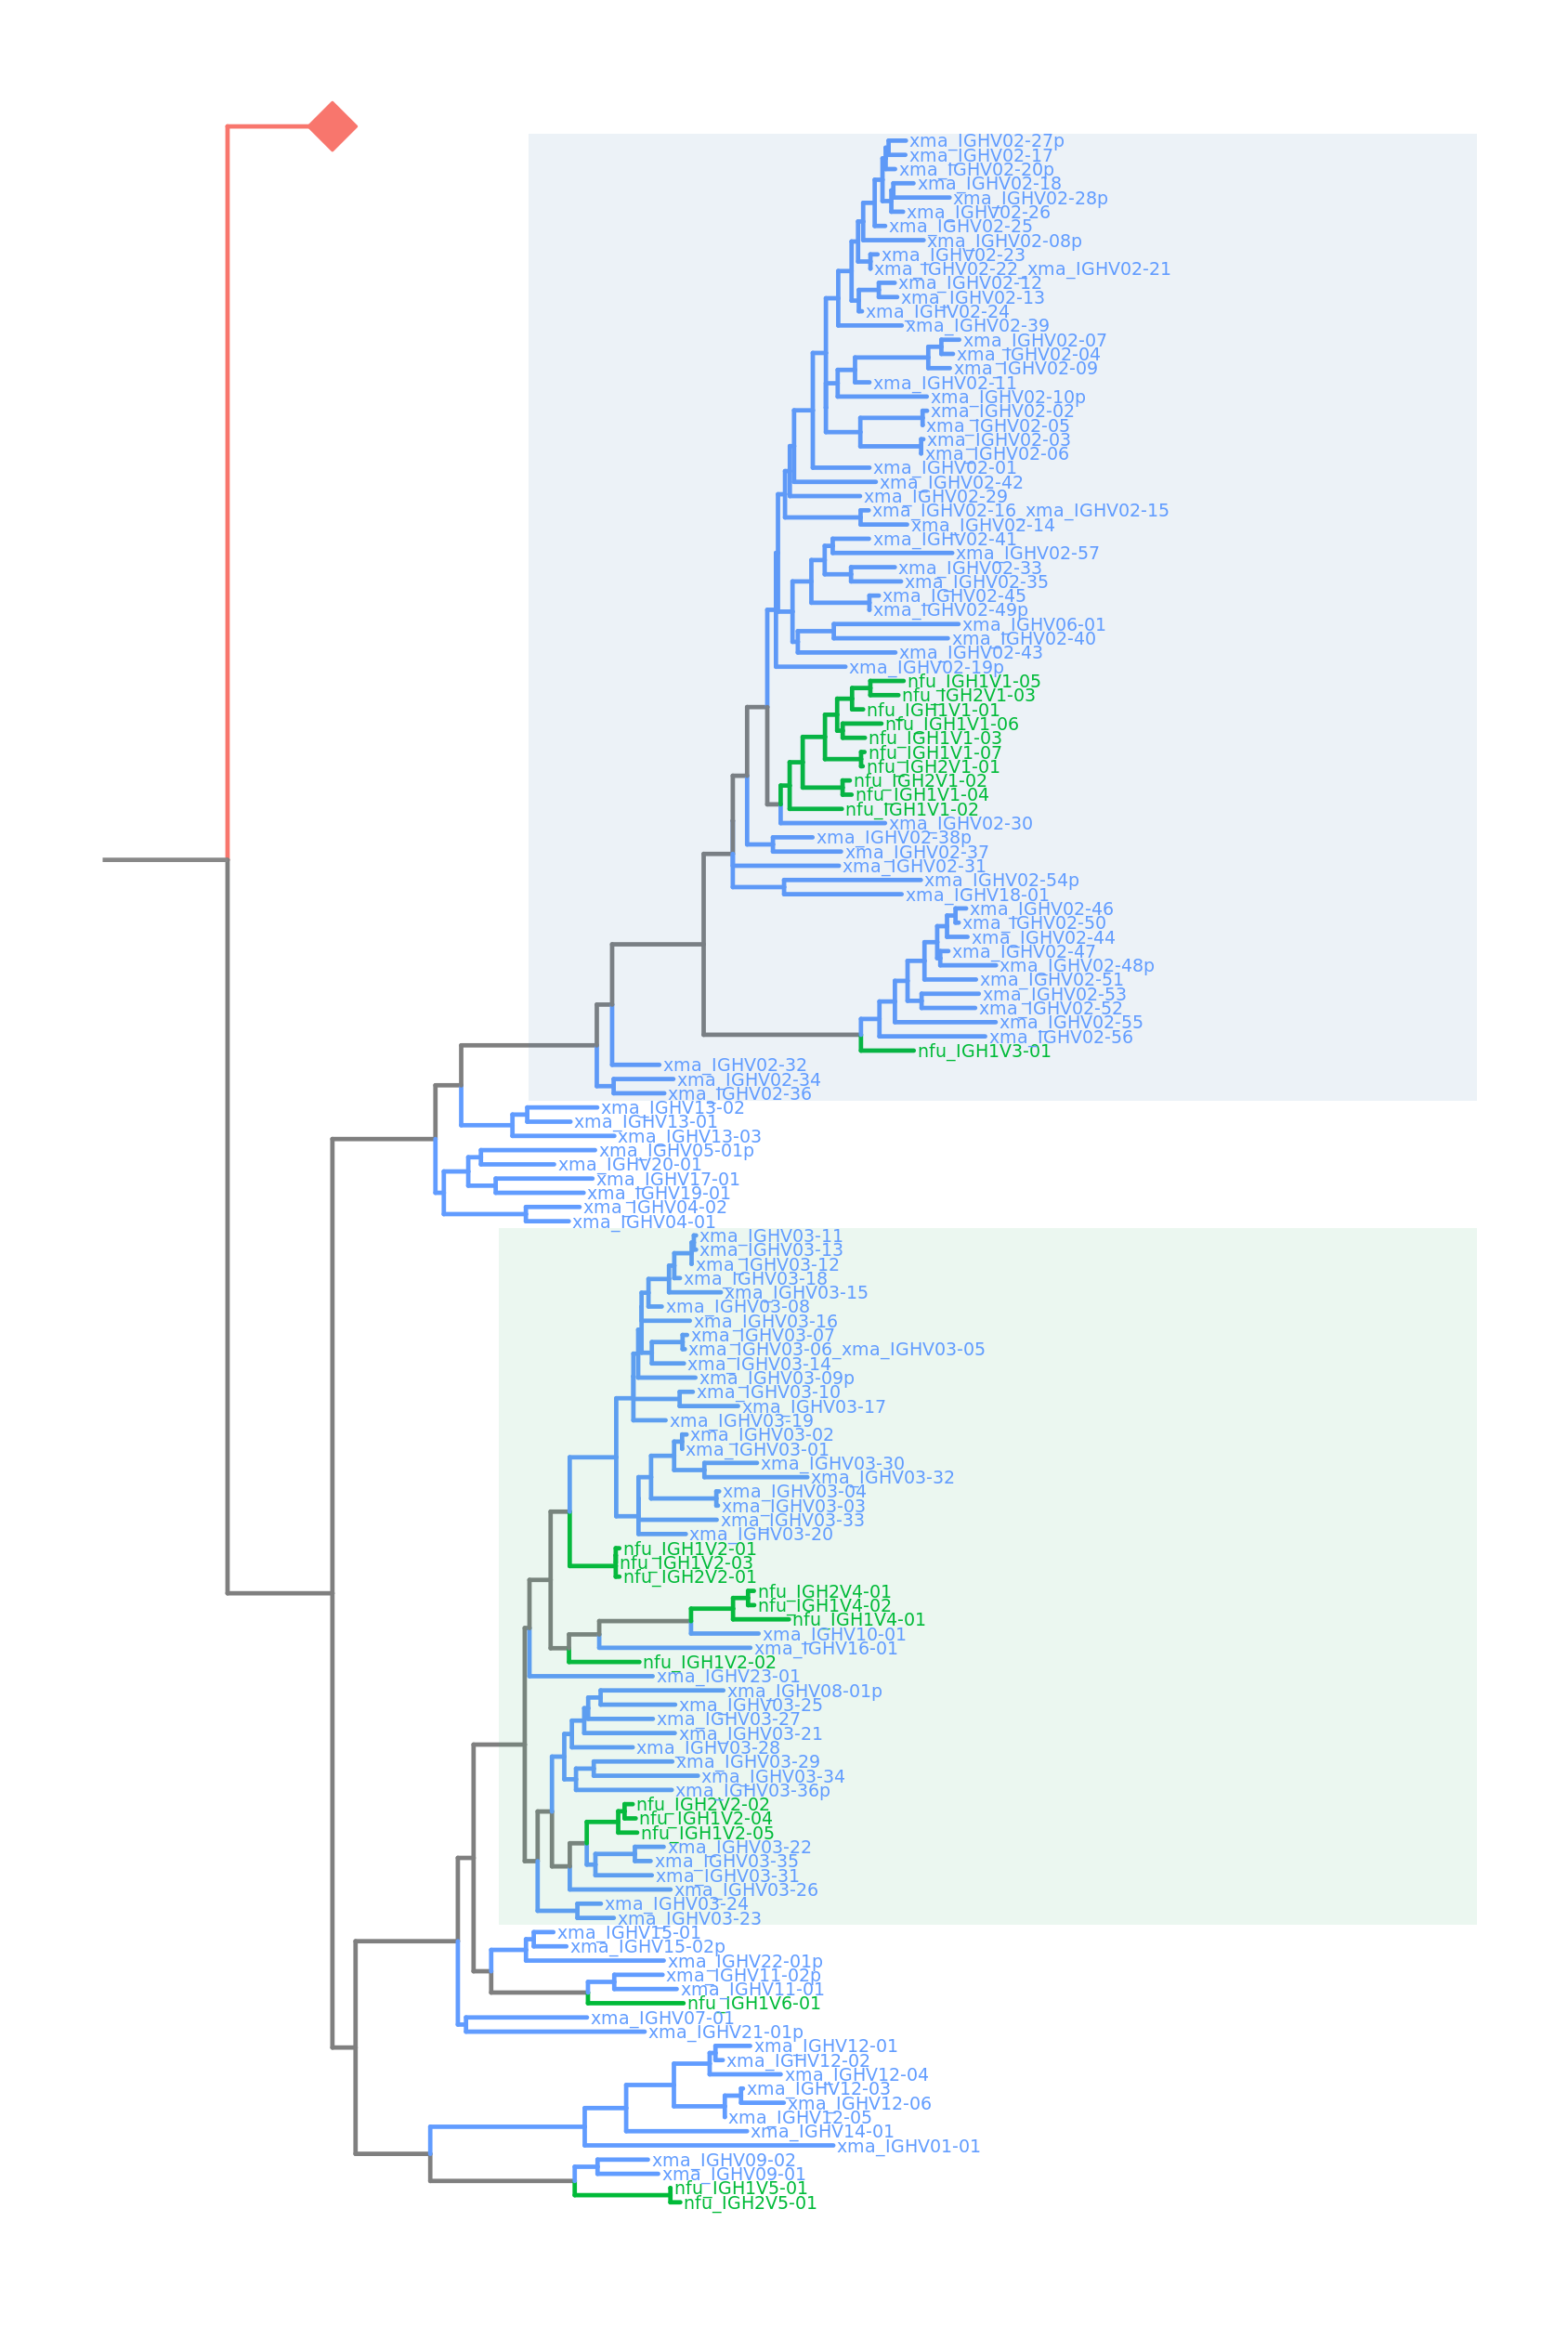
\includegraphics[width=0.8\textwidth]{_Figures/png/nfu-xma-vh-tree-nt.png} % TODO: AA tree in supplementary?
	\caption[Evolutionary relationships between \vh families in \Xma and \Nfu]{\textbf{Evolutionary relationships between \vh families in \Xma and \Nfu:} Phylogenetic tree of evolutionary relationships between \textit{IGH} \vh segments in \Nfu and \Xma, as inferred from the nucleotide sequences of \vh segments from both loci. Note the close interrelationship between the largest (blue zone) and second-largest (green zone) families in each species. The red diamond indicates the location of the outgroup, which is composed of zebrafish \textit{TRB} V-segments.}
	\label{fig:nfu-xma-vh-tree-nt}
	\end{figure}
	
	\begin{figure}
		\begin{subfigure}{0em}
        \phantomsubcaption{}
        \label{fig:xma-rss-seqlogo-all-heptamer}
    \end{subfigure}
    \begin{subfigure}{0em}
        \phantomsubcaption{}
        \label{fig:xma-rss-seqlogo-all-spacer}
    \end{subfigure}
    \begin{subfigure}{0em}
        \phantomsubcaption{}
        \label{fig:xma-rss-seqlogo-all-nonamer}
    \end{subfigure}
	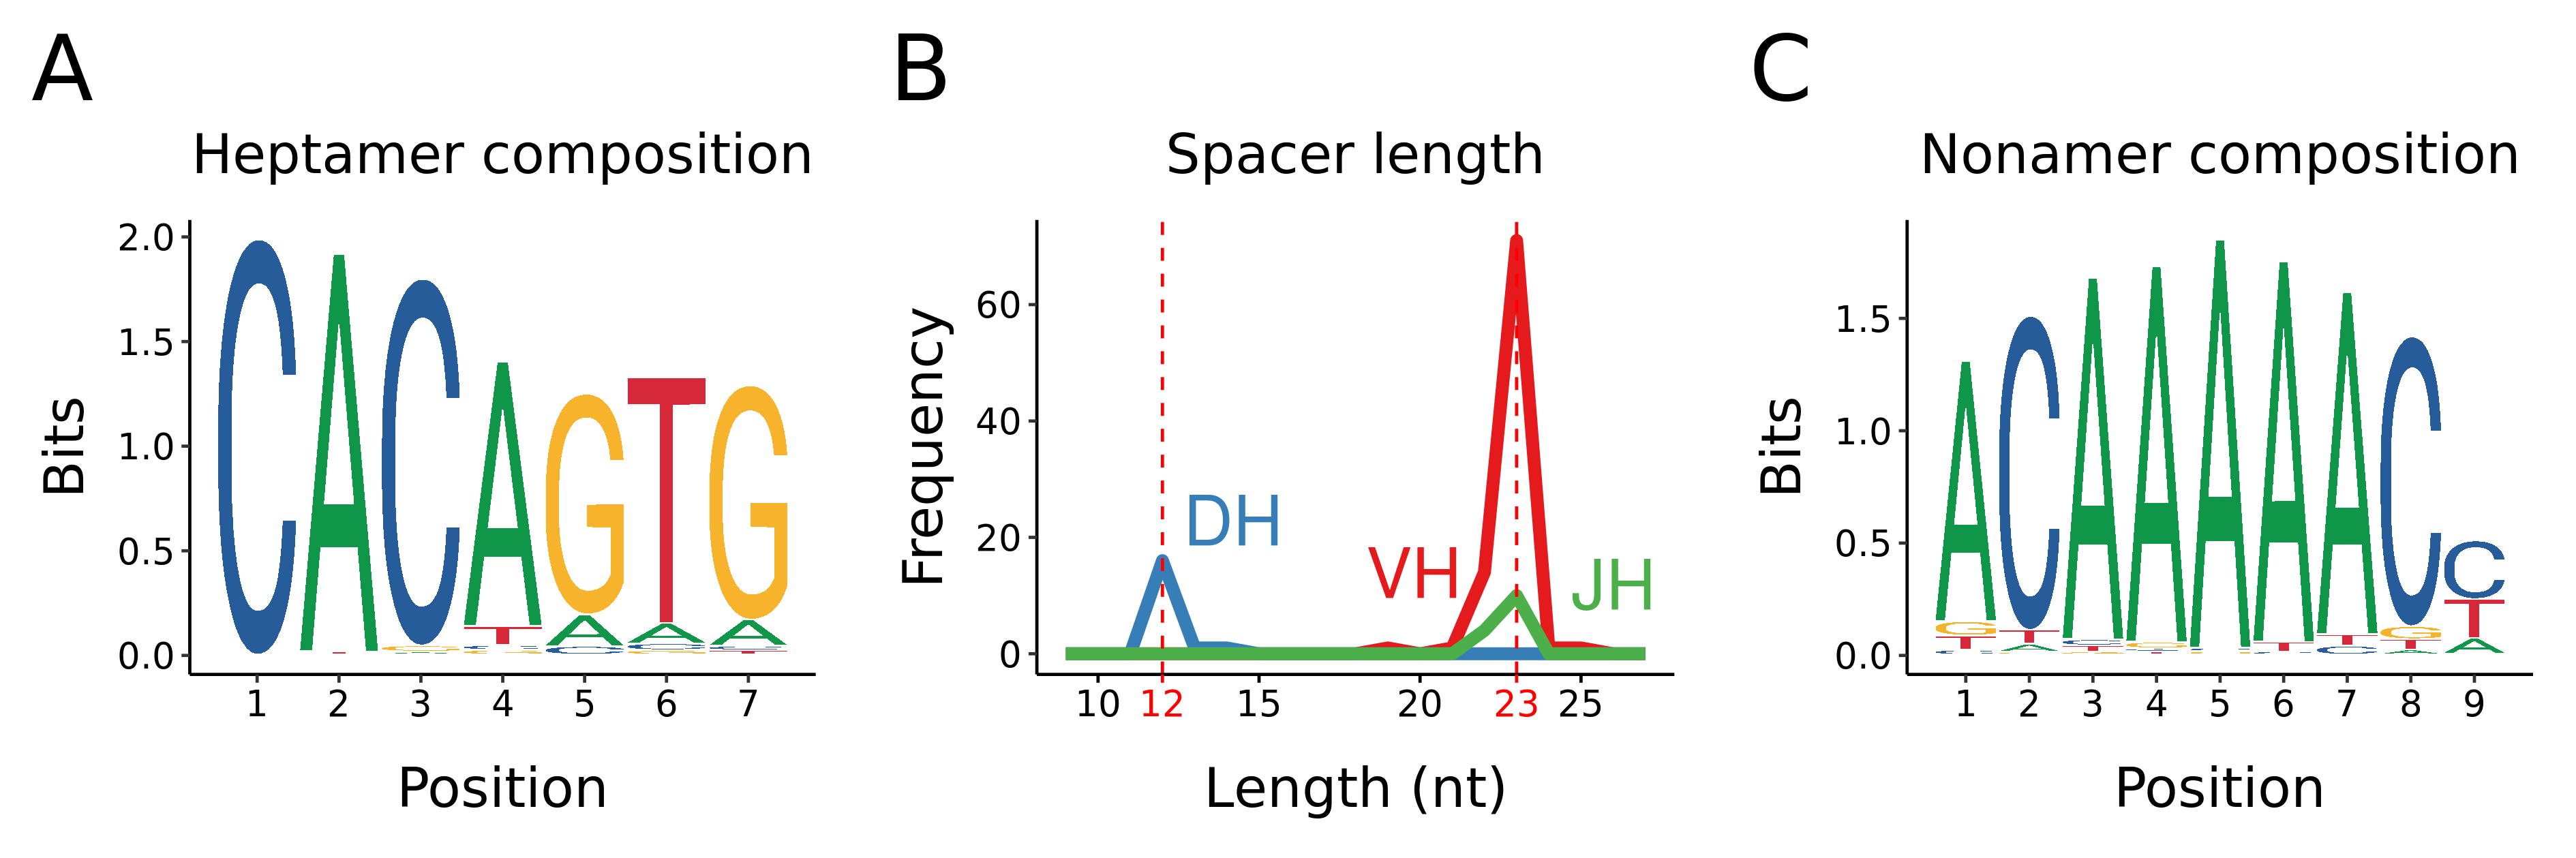
\includegraphics[width=\textwidth]{_Figures/png/xma-rss-seqlogo-all}
	\caption[Recombination signal sequences in the \Xma \textit{IGH} locus]{\textbf{Recombination signal sequences in the \Xma \textit{IGH} locus:} (A) Sequence composition of conserved heptamer sequences across all \Xma heavy-chain RSSs; (B) length distribution of unconserved spacer sequences in \Xma heavy-chain RSSs; (C) sequence composition of conserved heptamer sequences across all \Xma heavy-chain RSSs.}
	\label{fig:xma-rss-seqlogo-all}
	\end{figure}
	% TODO: Add in supplementary figure of heptamer/nonamer sequences separated by segment type

	%\subsection{Discussion} % Do I need this?	


\section{Comparitive analysis of \textit{IgH} constant-region structure in the Cyprinodontiformes}
\label{sec:comparative-loci}

	\subsection{Evolutionary history of IgZ}
	
	\subsection{Sublocus multiplicity and orientation}
	
	\subsection{Exon usage in transmembrane IgM \& other isoforms}
	
	
	
\begin{subappendices}
\section{Supplementary figures}
\dots
\section{Supplementary tables}

\afterpage{%
    \clearpage% Flush earlier floats (otherwise order might not be correct)
    %\thispagestyle{empty}% empty page style (?)
    \begin{landscape}% Landscape page
        \centering % Center table
        \vspace*{\fill}
        \scriptsize
		% latex table generated in R 3.5.2 by xtable 1.8-3 package
% Tue Jan 15 17:07:52 2019
\begin{tabular}{lrrrlrlrlrrl}
  \toprule Name & Start & End & Length & Strand & RSS Start & Heptamer & Spacer Length & Nonamer & RSS End & RSS Length & Comment \\ 
  \midrule IGH1V1-01 & 1252 & 1540 & 289 & + & 1541 & CACAGTG & 22 & ACAAAAACC & 1578 & 38 &  \\ 
  IGH1V1-02 & 3365 & 3656 & 292 & + & 3657 & CACAGTG & 22 & ACAAAAACC & 3694 & 38 &  \\ 
  IGH1V2-01 & 5907 & 6201 & 295 & + & 6202 & CACAGAA & 15 & ACAAAAACT & 6232 & 31 &  \\ 
  IGH1V1-03 & 13690 & 13964 & 275 & + & 13965 & CACAGTG & 22 & ACAAAAACC & 14002 & 38 &  \\ 
  IGH1V3-01 & 14862 & 15162 & 301 & + & 15163 & CACAGTG & 23 & ACAAAAACC & 15201 & 39 &  \\ 
  IGH1V2-02 & 17433 & 17730 & 298 & + & 17731 & CACAATG & 23 & ACAAAAACC & 17769 & 39 &  \\ 
  IGH1V4-01p & 24566 & 24837 & 272 & + & 24838 & CGCAGTG & 22 & CCACAAACC & 24875 & 38 & Nonsense mutation \\ 
  IGH1V1-04 & 37305 & 37596 & 292 & + & 37597 & CACAGTG & 22 & ACAAAAACC & 37634 & 38 &  \\ 
  IGH1V2-03 & 48845 & 49139 & 295 & + & 49140 & CACAGTG & 23 & TCAAAAACT & 49178 & 39 &  \\ 
  IGH1V1-05 & 49909 & 50197 & 289 & + & 50198 & CACAGTG & 22 & ACAAAAACC & 50235 & 38 &  \\ 
  IGH1V5-01 & 51710 & 51998 & 289 & + & 51999 & CACAGTG & 22 & ACAAAAACT & 52036 & 38 &  \\ 
  IGH1V2-04 & 56322 & 56616 & 295 & + & 56617 & CACAGTG & 23 & ACAAAAACC & 56655 & 39 &  \\ 
  IGH1V6-01 & 57465 & 57762 & 298 & + & 57763 & CACAGTG & 21 & ACTAAATCT & 57799 & 37 &  \\ 
  IGH1V1-06 & 59678 & 59966 & 289 & + & 59967 & CACAGTG & 22 & ACAAAAACC & 60004 & 38 &  \\ 
  IGH1V4-02p & 68017 & 68288 & 272 & + & 68289 & TGCAGTG & 22 & TCACAAACC & 68326 & 38 & Nonsense mutation \\ 
  IGH1V2-05 & 69787 & 70084 & 298 & + & 70085 & CACAGTG & 23 & ACAAAAACC & 70123 & 39 &  \\ 
  IGH1V1-07 & 155485 & 155763 & 279 & + & 155764 & CACAGTG & 22 & TCAAAACCC & 155801 & 38 &  \\ 
  IGH2V2-02 & 282620 & 282914 & 295 & - & 282915 & CACAGTG & 23 & ACAAAAACC & 282953 & 39 &  \\ 
  IGH2V4-01p & 284404 & 284675 & 272 & - & 284676 & TGCAGTG & 22 & TCACAAACC & 284713 & 38 & Nonsense mutation \\ 
  IGH2V5-01 & 288808 & 289096 & 289 & - & 289097 & CACAGTG & 22 & ACAGAAACT & 289134 & 38 &  \\ 
  IGH2V1-03 & 289977 & 290271 & 295 & - & 290272 & CACAGTG & 22 & ACAAAAACC & 290309 & 38 &  \\ 
  IGH2V1-02 & 293835 & 294126 & 292 & - & 294127 & CACAGTG & 22 & ACAAAAACC & 294164 & 38 &  \\ 
  IGH2V2-01 & 303780 & 304074 & 295 & - & 304075 & CAGGGCC & 24 & AGCACAAAG & 304114 & 40 &  \\ 
  IGH2V1-01 & 304926 & 305204 & 279 & - & 305205 & CACAGTG & 22 & TCAAAACCC & 305242 & 38 &  \\ 
   \bottomrule \end{tabular}

		\normalsize\vspace{1em}
        \captionof{table}{Co-ordinate table of \vh segments in the \nfu \igh{} locus}
        \vspace*{\fill}
    \end{landscape}
    \clearpage% Flush page
}

\afterpage{%
    \clearpage% Flush earlier floats (otherwise order might not be correct)
    %\thispagestyle{empty}% empty page style (?)
    \begin{landscape}% Landscape page
        \vspace*{0.5em}
        \centering % Center table
        \scriptsize
		% latex table generated in R 3.5.2 by xtable 1.8-3 package
% Tue Jan 15 17:07:52 2019
\begin{tabular}{lrlrrl}
  \toprule Name & Start & NT Sequence & End & Length & Strand \\ 
  \midrule IGH1D01 & 25782 & ATACGTACTTTCGTGGTATATAGAGA & 25807 & 26 & + \\ 
  IGH1D02 & 76700 & GATATCTGGGTGGGGG & 76715 & 16 & + \\ 
  IGH1D03 & 77027 & TGAAATGATTAC & 77038 & 12 & + \\ 
  IGH1D04 & 77476 & TCGCGTAGCGGC & 77487 & 12 & + \\ 
  IGH1D05 & 78717 & GAAACCACGGCAGC & 78730 & 14 & + \\ 
  IGH1D06 & 79049 & TTTATAGCGGCTAC & 79062 & 14 & + \\ 
  IGH1D07 & 80417 & CAGACTGGAGA & 80427 & 11 & + \\ 
  IGH1D08 & 81362 & TTCATGGCAGCCAC & 81375 & 14 & + \\ 
  IGH1D09 & 82067 & CAGACTGGAGC & 82077 & 11 & + \\ 
  IGH1D10 & 84282 & TGGGGTGGCAGC & 84293 & 12 & + \\ 
  IGH2D04 & 263497 & CAGACTGGAGA & 263507 & 11 & - \\ 
  IGH2D03 & 270243 & TTTATAGCGGCTAC & 270256 & 14 & - \\ 
  IGH2D02 & 270878 & GAAACCACGGCAGC & 270891 & 14 & - \\ 
  IGH2D01 & 271749 & GACTTTTACTAC & 271760 & 12 & - \\ 
   \bottomrule \end{tabular}

		\normalsize\vspace{1em}
        \captionof{table}{Co-ordinate table of \dh segments in the \nfu \igh{} locus}
        \scriptsize
		% latex table generated in R 3.5.1 by xtable 1.8-3 package
% Tue Dec 18 15:50:37 2018
\begin{tabular}{l|rlrlr|rlrlr}\toprule
  \multirow{2}{*}{Name} & \multicolumn{5}{c|}{5'-RSS} & \multicolumn{5}{c}{3'-RSS} \\
    ~ & Start & Nonamer & Spacer length & Heptamer & End & Start & Heptamer & Spacer length & Nonamer & End \\\midrule
  IGH1D01 & 25754 & GGTTGTTGT & 12 & CACTGTG & 25781 & 25808 & CACAGTG & 12 & ACAAAAACC & 25835 \\ 
  IGH1D02 & 76672 & AGTTTTTGA & 12 & CACAGTG & 76700 & 76716 & CACAGTG & 12 & ACAAAAACC & 76743 \\ 
  IGH1D03 & 76999 & TGTTGTTGT & 12 & CACAGTG & 77026 & 77039 & CACTGTG & 11 & AATATAACC & 77065 \\ 
  IGH1D04 & 77448 & AGTTTTTGT & 12 & CACGGTG & 77475 & 77488 & CACAGCG & 12 & ACATAAAAC & 77515 \\ 
  IGH1D05 & 78688 & GATGTTTTT & 13 & CACAGTG & 78716 & 78731 & CACAGCG & 12 & ACAAAAGCC & 78758 \\ 
  IGH1D06 & 79021 & TGTTTTTGT & 12 & CGCTGTG & 79048 & 79063 & CACTGTG & 12 & ACAAGATCC & 79090 \\ 
  IGH1D07 & 80389 & AGTTTTGGT & 12 & CACAGTG & 80416 & 80428 & CACAACG & 12 & ACAAAAACC & 80455 \\ 
  IGH1D08 & 81334 & TGTTTTTGT & 12 & CGCTGTG & 81361 & 81376 & CACTGTG & 12 & ACAAAATCC & 81403 \\ 
  IGH1D09 & 82039 & AGTTTTGGT & 12 & CACAGTG & 82066 & 82078 & CACAATG & 12 & ACAAAAACC & 82105 \\ 
  IGH1D10 & 84254 & TCATTCATT & 12 & CACTGTG & 84281 & 84294 & CACAGTG & 12 & ACAAAAACC & 84321 \\ 
  IGH2D04 & 263533 & AGTTTTGGT & 12 & CACAGTG & 263506 & 263494 & CACAACG & 12 & ACAAAAACC & 263467 \\ 
  IGH2D03 & 270282 & TGTTTTTGT & 12 & CGCTGTG & 270255 & 270240 & CACTGTG & 12 & ACAAGATCC & 270213 \\ 
  IGH2D02 & 270917 & TGTTTTTGT & 12 & CACAGTG & 270890 & 270875 & CACAGCG & 12 & ACAAAAGCC & 270848 \\ 
  IGH2D01 & 271786 & AGTTTTTAT & 12 & CATGGTG & 271759 & 271746 & CACAATG & 12 & ACAAAAACC & 271719 \\ 
   \bottomrule \end{tabular}

		\normalsize\vspace{1em}
        \captionof{table}{Co-ordinate table of \dh RSSs in the \nfu \igh{} locus}
        \vspace*{0.5em}
    \end{landscape}
    \clearpage% Flush page
}

\afterpage{%
    \clearpage% Flush earlier floats (otherwise order might not be correct)
    %\thispagestyle{empty}% empty page style (?)
    \begin{landscape}% Landscape page
        \vspace*{0.5em}
        \centering % Center table
        \notsotiny
		% latex table generated in R 3.5.2 by xtable 1.8-3 package
% Tue Jan 15 17:07:52 2019
\begin{tabular}{lrllrrl}
  \toprule Name & Start & NT Sequence & AA Sequence & End & Length & Strand \\ 
  \midrule IGH1J01 & 26187 & GTGCTTTAGACAACTGGGGAAAAGGAACGGAGGTTACTGTTCAACCTG & ALDNWGKGTEVTVQP & 26234 & 48 & + \\ 
  IGH1J02 & 128176 & ATGACTACTTTGACTACTGGGGAAAAGGAACAATGGTGACGGTCACATCAG & DYFDYWGKGTMVTVTS & 128226 & 51 & + \\ 
  IGH1J03 & 128354 & ACCGTGGGGTAAAGGGACAACAGTCACGGTCAAAACAG & PWGKGTTVTVKT & 128391 & 38 & + \\ 
  IGH1J04 & 128533 & ACGGTGCTCTTGACTACTGGGGTAAAGGGACCGCAGTCACTGTAACATCAG & GALDYWGKGTAVTVTS & 128583 & 51 & + \\ 
  IGH1J05 & 128887 & ACAACGCTTTTGACTACTGGGGAAAAGGAACAACGGTCACCGTCACTTCAG & NAFDYWGKGTTVTVTS & 128937 & 51 & + \\ 
  IGH1J06 & 129346 & CTACGATGCTTTTGACTACTGGGGGAAAAGGACGATGGTCACGTCACTTCAG & YDAFDYWGKRTMVTSLQ & 129397 & 52 & + \\ 
  IGH1J07 & 129635 & TTAACTGGGCTTTCGACTACTGGGGAAAAGGGACGATGGTAACGGTGACTTCAG & NWAFDYWGKGTMVTVTS & 129688 & 54 & + \\ 
  IGH1J08 & 129965 & TTACCACGCAGCTTTGGACTACTGGGGAAAAGGGACGACGGTCACCGTCACCTCAG & YHXALDYWGKGTTVTVTS & 130020 & 56 & + \\ 
  IGH1J09 & 130612 & TCTACGCTGCTTTTGACTACTGGGGTAAAGGTACAACGGTAACCGTTTCATCAG & YAAFDYWGKGTTVTVSS & 130665 & 54 & + \\ 
  IGH2J08 & 204031 & TCTACGCTGCTTTTGACTACTGGGGTAAAGGTACAACGGTAACCGTTTCATCAG & YAAFDYWGKGTTVTVSS & 204084 & 54 & - \\ 
  IGH2J07 & 204673 & TTACCACGCAGCTTTGGACTACTGGGGAAAAGGGACGACGGTCACCGTCACCTCAG & YHXALDYWGKGTTVTVTS & 204728 & 56 & - \\ 
  IGH2J06 & 205005 & ATAACTGGGCTTTCGACTACTGGGGAAAAGGGACGATGGTAACGGTGACTTCAG & NWAFDYWGKGTMVTVTS & 205058 & 54 & - \\ 
  IGH2J05 & 205296 & CTACGATGCTTTTGACTACTGGGGGAAAAGGACGATGGTCACGTCACTTCAG & YDAFDYWGKRTMVTSLQ & 205347 & 52 & - \\ 
  IGH2J04 & 205756 & ACAACGCTTTTGACTACTGGGGAAAAGGAACAACGGTCACCGTCACTTCAG & NAFDYWGKGTTVTVTS & 205806 & 51 & - \\ 
  IGH2J03 & 206111 & ATGGTGCTTTTGACTACTGGGGTAAAGGGACCGCAGTCACTGTAACATCAG & GAFDYWGKGTAVTVTS & 206161 & 51 & - \\ 
  IGH2J02 & 206303 & ACCGTGGGGTAAAGGGACAACAGTCACGGTCAAAACAG & PWGKGTTVTVKT & 206340 & 38 & - \\ 
  IGH2J01 & 206466 & ATGACTACTTTGACTACTGGGGAAAAGGAACAATGGTGACGGTCACATCAG & DYFDYWGKGTMVTVTS & 206516 & 51 & - \\ 
   \bottomrule \end{tabular}

		\normalsize\vspace{1em}
        \captionof{table}{Co-ordinate table of \jh segments in the \nfu \igh{} locus}
        \notsotiny
		% latex table generated in R 3.5.2 by xtable 1.8-3 package
% Tue Jan 15 17:07:52 2019
\begin{tabular}{lrlrlrr}
  \toprule Name & RSS Start & Nonamer & Spacer Length & Heptamer & RSS End & RSS Length \\ 
  \midrule IGH1J01 & 26196 & TGTTTTTGT & 23 & CACTGTG & 26186 & 39 \\ 
  IGH1J02 & 128188 & AGTGTTTGT & 23 & CACTGTG & 128175 & 39 \\ 
  IGH1J03 & 128353 & TGTTTATTT & 23 & CACTGTG & 128353 & 39 \\ 
  IGH1J04 & 128545 & GGTTTTTGT & 23 & CACTGTG & 128532 & 39 \\ 
  IGH1J05 & 128899 & GGTTTTAGT & 23 & TACTGTG & 128886 & 39 \\ 
  IGH1J06 & 129360 & TCTTCTTGT & 22 & TACTTTG & 129345 & 38 \\ 
  IGH1J07 & 129650 & AGTTTTTGT & 23 & TACTGTG & 129634 & 39 \\ 
  IGH1J08 & 129983 & AGTTTTAGT & 22 & TACTGTG & 129964 & 38 \\ 
  IGH1J09 & 130628 & CGTTTTTAT & 22 & CACTGTG & 130611 & 38 \\ 
  IGH2J08 & 204047 & CGTTTTTAT & 22 & CACTGTG & 204030 & 38 \\ 
  IGH2J07 & 204691 & AGTTTTAGT & 22 & TACTGTG & 204672 & 38 \\ 
  IGH2J06 & 205020 & AGTTTTTGT & 23 & TACTGTG & 205004 & 39 \\ 
  IGH2J05 & 205310 & TCTTCTTGT & 22 & TACTTTG & 205295 & 38 \\ 
  IGH2J04 & 205768 & GGTTTTAGT & 23 & TACTGTG & 205755 & 39 \\ 
  IGH2J03 & 206123 & GGTTTTTGT & 23 & CACTGTG & 206110 & 39 \\ 
  IGH2J02 & 206302 & TGTTTATTT & 23 & CACTGTG & 206302 & 39 \\ 
  IGH2J01 & 206478 & AGTGTTTGT & 23 & CACTGTG & 206465 & 39 \\ 
   \bottomrule \end{tabular}

		\normalsize\vspace{1em}
        \captionof{table}{Co-ordinate table of \jh RSSs in the \nfu \igh{} locus}
        \vspace*{0.5em}
    \end{landscape}
    \clearpage% Flush page
}

\afterpage{%
    \clearpage% Flush earlier floats (otherwise order might not be correct)
    %\thispagestyle{empty}% empty page style (?)
    \begin{landscape}% Landscape page
        \centering % Center table
        \vspace*{\fill}
        \scriptsize
		% latex table generated in R 3.5.1 by xtable 1.8-3 package
% Mon Dec 24 16:20:22 2018
\begin{tabular}{lrrrlrlllrrl}
  \toprule Name & Start & End & Length & Strand & RSS Start & Heptamer & Spacer Length & Nonamer & RSS End & RSS Length & Comment \\ 
  \midrule IGHV01-01 & 1159 & 1450 & 292 & + & 1451 & CACAGTG & 23 & GTAAAAACC & 1489 & 39 &  \\ 
  IGHV02-01 & 10534 & 10825 & 292 & + & 10826 & CACAGTG & 23 & ACAAAACCC & 10864 & 39 &  \\ 
  IGHV02-02 & 11961 & 12261 & 301 & + & 12262 & CACTGTG & 23 & ACAAAAACT & 12300 & 39 &  \\ 
  IGHV02-03 & 13319 & 13616 & 298 & + & 13617 & CACAGTG & 23 & ACACAAACT & 13655 & 39 &  \\ 
  IGHV03-01 & 15440 & 15734 & 295 & + & 15735 & CACAGTG & 22 & ACAAAAACT & 15772 & 38 &  \\ 
  IGHV02-04 & 16618 & 16908 & 291 & + & 16909 & CACAGTG & 23 & ACAAAAACC & 16947 & 39 &  \\ 
  IGHV02-05 & 17522 & 17822 & 301 & + & 17823 & CACTGTG & 22 & ACAAAAACT & 17860 & 38 &  \\ 
  IGHV02-06 & 18881 & 19178 & 298 & + & 19179 & CACAGTG & 23 & ACACAAACT & 19217 & 39 &  \\ 
  IGHV03-02 & 21000 & 21294 & 295 & + & 21295 & CACAGTG & 22 & ACAAAAACT & 21332 & 38 &  \\ 
  IGHV02-07 & 22179 & 22467 & 289 & + & 22468 & CACAGTG & 23 & ACAAAAACC & 22506 & 39 &  \\ 
  IGHV02-08p & 24234 & 24514 & 281 & + & 24515 & CACAGTG & 23 & ACAAAAACT & 24553 & 39 & Frameshift \\ 
  IGHV04-01 & 25359 & 25659 & 301 & + & 25660 & CACAGTG & 23 & ACAAAAACT & 25698 & 39 &  \\ 
  IGHV04-02 & 27066 & 27366 & 301 & + & 27367 & CACAGTG & 23 & ACAAAAACA & 27405 & 39 &  \\ 
  IGHV02-09 & 28669 & 28958 & 290 & + & 28959 & CACAGTG & 23 & ACAAAAACC & 28997 & 39 &  \\ 
  IGHV02-10p & 30460 & 30741 & 282 & + & 30742 & CACAATG & 23 & ACAAAACTC & 30780 & 39 & Frameshift \\ 
  IGHV02-11 & 32395 & 32681 & 287 & + & 32682 & CACAGTG & 23 & ACAAAAACC & 32720 & 39 &  \\ 
  IGHV03-03 & 33663 & 33957 & 295 & + & 33958 & CACTGTG & 22 & ACAAAAACT & 33995 & 38 &  \\ 
  IGHV02-12 & 35012 & 35299 & 288 & + & 35300 & CACAGTG & 23 & ACAAAAACC & 35338 & 39 &  \\ 
  IGHV03-04 & 36281 & 36575 & 295 & + & 36576 & CACTGTG & 22 & ACAAAAACT & 36613 & 38 &  \\ 
  IGHV02-13 & 37639 & 37931 & 293 & + & 37932 & CACAGTG & 23 & ACAAAAACT & 37970 & 39 &  \\ 
  IGHV02-14 & 39019 & 39311 & 293 & + & 39312 & CACAGTG & 23 & ACAAAAACT & 39350 & 39 &  \\ 
  IGHV03-05 & 41008 & 41302 & 295 & + & 41303 & CACAGTG & 22 & ACAAAAACT & 41340 & 38 &  \\ 
  IGHV02-15 & 42660 & 42952 & 293 & + & 42953 & CACAGTG & 23 & ACAAAAACT & 42991 & 39 &  \\ 
  IGHV03-06 & 45081 & 45375 & 295 & + & 45376 & CACAGTG & 22 & ACAAAAACT & 45413 & 38 &  \\ 
  IGHV02-16 & 46732 & 47024 & 293 & + & 47025 & CACAGTG & 23 & ACAAAAACT & 47063 & 39 &  \\ 
  IGHV03-07 & 48618 & 48912 & 295 & + & 48913 & CACAGTG & 22 & ACAAAAACT & 48950 & 38 &  \\ 
  IGHV02-17 & 50323 & 50611 & 289 & + & 50612 & CACAGTG & 23 & ACAAAAACC & 50650 & 39 &  \\ 
  IGHV03-08 & 51890 & 52184 & 295 & + & 52185 & CACAGTG & 22 & ACAAAAACT & 52222 & 38 &  \\ 
  IGHV03-09p & 53026 & 53274 & 249 & + & 53275 &  &  &  &  &  & 3'-truncated, no RSS \\ 
  IGHV02-18 & 54462 & 54747 & 286 & + & 54748 & CACAGTG & 23 & ACAAAAACC & 54786 & 39 &  \\ 
  IGHV02-19p & 55729 & 55866 & 138 & + & 55867 & CACAGTG & 23 & ACAAAAACC & 55905 & 39 & 3'-truncated \\ 
  IGHV03-10 & 57371 & 57662 & 292 & + & 57663 & CACAGTG & 22 & ACAAAAACT & 57700 & 38 &  \\ 
  IGHV02-20p & 58698 & 58986 & 289 & + & 58987 & CACAGTG & 23 & ATAAAAACC & 59025 & 39 & Nonsense mutation \\ 
  IGHV03-11 & 59940 & 60234 & 295 & + & 60235 & CACAGTG & 22 & ACAAAAACT & 60272 & 38 &  \\ 
  IGHV02-21 & 61249 & 61537 & 289 & + & 61538 & CACAGTG & 23 & ATAAAAACC & 61576 & 39 &  \\ 
  IGHV03-12 & 62491 & 62785 & 295 & + & 62786 & CACAGTG & 22 & ACAAAAACT & 62823 & 38 &  \\ 
  IGHV02-22 & 63801 & 64089 & 289 & + & 64090 & CACAGTG & 23 & ATAAAAACC & 64128 & 39 &  \\ 
  IGHV03-13 & 65043 & 65337 & 295 & + & 65338 & CACAGTG & 22 & ACAAAAACT & 65375 & 38 &  \\ 
  IGHV02-23 & 66354 & 66640 & 287 & + & 66641 & CACAGTG & 23 & ACAAAAACT & 66679 & 39 &  \\ 
  IGHV03-14 & 68452 & 68743 & 292 & + & 68744 & CACTATG & 22 & ACAAAACTC & 68781 & 38 &  \\ 
  IGHV02-24 & 70101 & 70389 & 289 & + & 70390 & CACAGTG & 23 & ACAAAAACC & 70428 & 39 &  \\ 
  IGHV03-15 & 72206 & 72501 & 296 & + & 72502 & CACAGTG & 22 & ACAAAAACT & 72539 & 38 &  \\ 
  IGHV02-25 & 73484 & 73772 & 289 & + & 73773 & CACAGTG & 23 & ACAAAAACC & 73811 & 39 &  \\ 
  IGHV03-16 & 75799 & 76090 & 292 & + & 76091 & CACAGTG & 22 & ACAAAAACT & 76128 & 38 &  \\ 
  IGHV03-17 & 77773 & 78067 & 295 & + & 78068 & CACAGTG & 22 & ACAAAAACT & 78105 & 38 &  \\ 
  IGHV02-26 & 79001 & 79289 & 289 & + & 79290 & CACAGTG & 23 & ACAAAAACC & 79328 & 39 &  \\ 
  IGHV03-18 & 80492 & 80784 & 293 & + & 80785 & CACAGTG & 22 & ACAAAAACT & 80822 & 38 &  \\ 
  IGHV02-27p & 81799 & 82082 & 284 & + & 82083 & CACAGTG & 23 & ACAAAAACC & 82121 & 39 & Frameshift \\ 
  IGHV03-19 & 83736 & 84030 & 295 & + & 84031 & CACAGTG & 22 & ACAAAAACT & 84068 & 38 &  \\ 
  IGHV02-28p & 85093 & 85381 & 289 & + & 85382 & CACAGGG & 23 & GCAAAAACC & 85420 & 39 & Nonsense mutation \\ 
  IGHV02-29 & 86225 & 86505 & 281 & + & 86506 & CACAGTG & 23 & ATAAAAACC & 86544 & 39 &  \\ 
  IGHV03-20 & 87419 & 87713 & 295 & + & 87714 & CACAGTG & 22 & ACAAAAACT & 87751 & 38 &  \\ 
  IGHV03-21 & 94532 & 94826 & 295 & + & 94827 & CACAGTG & 23 & ACAAAAACC & 94865 & 39 &  \\ 
  IGHV03-22 & 96192 & 96489 & 298 & + & 96490 & CACAGTG & 23 & ACAAAAACC & 96528 & 39 &  \\ 
  IGHV03-23 & 98068 & 98368 & 301 & + & 98369 & CACAGTG & 23 & ACAAAAACC & 98407 & 39 &  \\ 
  IGHV03-24 & 99482 & 99779 & 298 & + & 99780 & CACAGTG & 23 & ACAAAAACC & 99818 & 39 &  \\ 
  IGHV03-25 & 101639 & 101936 & 298 & + & 101937 & CACAGTG & 23 & ACAAAAACC & 101975 & 39 &  \\ 
  IGHV05-01p & 102818 & 103096 & 279 & + & 103097 & CAGAAGC & 0 & ACAAAAACT & 103112 & 16 & Frameshift \\ 
  IGHV03-26 & 104098 & 104389 & 292 & + & 104390 & CACAGTG & 23 & ACAAAATCC & 104428 & 39 &  \\ 
  IGHV06-01 & 105551 & 105831 & 281 & + & 105832 & CACAGTG & 23 & ACAAAAACC & 105870 & 39 &  \\ 
  IGHV03-27 & 107274 & 107571 & 298 & + & 107572 & CACAGTG & 23 & ACAAAAACC & 107610 & 39 &  \\ 
  IGHV03-28 & 108775 & 109072 & 298 & + & 109073 & CACAGAG & 23 & ACAAAAACC & 109111 & 39 &  \\ 
  IGHV03-29 & 110372 & 110672 & 301 & + & 110673 & CACAGTG & 23 & ACAAAAACC & 110711 & 39 &  \\ 
  IGHV07-01 & 111565 & 111856 & 292 & + & 111857 & CACAATG & 23 & ACAAAAACT & 111895 & 39 &  \\ 
  IGHV08-01p & 113033 & 113330 & 298 & + & 113331 & CACAGAG & 23 & CCAAGAACC & 113369 & 39 & Nonsense mutation \\ 
  IGHV09-01 & 115512 & 115800 & 289 & + & 115801 & CACAGTG & 22 & ACAAAAACT & 115838 & 38 &  \\ 
  IGHV10-01 & 117078 & 117379 & 302 & + & 117380 & CACAGTG & 22 & ACATAAACT & 117417 & 38 &  \\ 
  IGHV11-01 & 119462 & 119760 & 299 & + & 119761 & CACAGTG & 23 & ACAAAAACT & 119799 & 39 &  \\ 
  IGHV03-30 & 126125 & 126416 & 292 & + & 126417 & CACAGTG & 22 & ACAAAAACC & 126454 & 38 &  \\ 
  IGHV03-31 & 127109 & 127400 & 292 & + & 127401 & CACAGTG & 23 & GCAAAAACC & 127439 & 39 &  \\ 
  IGHV12-01 & 128489 & 128786 & 298 & + & 128787 & CACAGTG & 23 & ACAAAAACC & 128825 & 39 &  \\ 
  IGHV02-30 & 135711 & 136000 & 290 & + & 136001 & CACAGTG & 22 & ACAAAAACA & 136038 & 38 &  \\ 
  IGHV13-01 & 136757 & 137057 & 301 & + & 137058 & CACAGTG & 23 & ACAAAAACT & 137096 & 39 &  \\ 
  IGHV02-31 & 138344 & 138637 & 294 & + & 138638 & CACAGTG & 23 & ACAAAAATC & 138676 & 39 &  \\ 
  IGHV02-32 & 140024 & 140315 & 292 & + & 140316 & CACTGTG & 23 & ACAAAAACT & 140354 & 39 &  \\ 
  IGHV02-33 & 142332 & 142620 & 289 & + & 142621 & CACAGTG & 23 & ACAAAAACA & 142659 & 39 &  \\ 
  IGHV02-34 & 144334 & 144625 & 292 & + & 144626 & CACAGTG & 23 & ACAAAAACT & 144664 & 39 &  \\ 
  IGHV02-35 & 145740 & 146031 & 292 & + & 146032 & CACAGTG & 23 & ACAAAAAAT & 146070 & 39 &  \\ 
  IGHV02-36 & 146903 & 147194 & 292 & + & 147195 & CACAGTG & 23 & ACAAAAACT & 147233 & 39 &  \\ 
  IGHV02-37 & 147839 & 148138 & 300 & + & 148139 & CACAGTG & 23 & ACAAAAATC & 148177 & 39 &  \\ 
  IGHV02-38p & 150504 & 150797 & 294 & + & 150798 & CACAATA & 23 & ACAAAAACC & 150836 & 39 & Nonsense mutation \\ 
  IGHV02-39 & 152249 & 152537 & 289 & + & 152538 & CACAGTA & 23 & ACAAAAACC & 152576 & 39 &  \\ 
  IGHV14-01 & 154075 & 154374 & 300 & + & 154375 & CACAGTG & 23 & ACAAAAAGT & 154413 & 39 &  \\ 
  IGHV02-40 & 155433 & 155709 & 277 & + & 155710 & CACAGTG & 23 & ACAAAAACC & 155748 & 39 &  \\ 
  IGHV02-41 & 156583 & 156870 & 288 & + & 156871 & CACAGTG & 23 & ACAAAAACC & 156909 & 39 &  \\ 
  IGHV02-42 & 163977 & 164269 & 293 & + & 164270 & CACAGTG & 23 & ACAAAACCC & 164308 & 39 &  \\ 
  IGHV03-32 & 165416 & 165708 & 293 & + & 165709 & CACAGTG & 22 & ACAAAAACA & 165746 & 38 &  \\ 
  IGHV02-43 & 166994 & 167293 & 300 & + & 167294 & CACAATG & 23 & ACAGAAACT & 167332 & 39 &  \\ 
  IGHV12-02 & 169602 & 169900 & 299 & + & 169901 & CACAGTG & 23 & ACAAAAACC & 169939 & 39 &  \\ 
  IGHV02-44 & 171452 & 171752 & 301 & + & 171753 & CACTGTG & 23 & GCAAAAACT & 171791 & 39 &  \\ 
  IGHV02-45 & 173096 & 173384 & 289 & + & 173385 & CTCAGTG & 23 & ACAAAAACC & 173423 & 39 &  \\ 
  IGHV02-46 & 174714 & 175009 & 296 & + & 175010 & CACAGTG & 23 & ACAAAAACT & 175048 & 39 &  \\ 
  IGHV02-47 & 176396 & 176697 & 302 & + & 176698 & CACAGTG & 23 & ACAAAAACT & 176736 & 39 &  \\ 
  IGHV12-03 & 178422 & 178719 & 298 & + & 178720 & CACAGTG & 23 & ACAAAAACA & 178758 & 39 &  \\ 
  IGHV12-04 & 181245 & 181543 & 299 & + & 181544 & CACAGTG & 23 & ACAAAAACC & 181582 & 39 &  \\ 
  IGHV02-48p & 182977 & 183236 & 260 & + & 183237 & CACAGGT & 8 & ACAAAAACT & 183260 & 24 & 5'-truncated \\ 
  IGHV02-49p & 184323 & 184611 & 289 & + & 184612 & CACAGTG & 23 & ACAAAAACC & 184650 & 39 & Nonsense mutation \\ 
  IGHV02-50 & 185946 & 186244 & 299 & + & 186245 & CACAGTG & 23 & ACAAAAACT & 186283 & 39 &  \\ 
  IGHV02-51 & 187624 & 187925 & 302 & + & 187926 & CACAGTG & 23 & ACAAAAACT & 187964 & 39 &  \\ 
  IGHV12-05 & 190987 & 191284 & 298 & + & 191285 & CACAGTG & 23 & ACAAAAACA & 191323 & 39 &  \\ 
  IGHV02-52 & 192570 & 192868 & 299 & + & 192869 & CACAGTG & 19 & CTGAAAACC & 192903 & 35 &  \\ 
  IGHV12-06 & 193608 & 193906 & 299 & + & 193907 & CACAGTG & 23 & ACAAAAACA & 193945 & 39 &  \\ 
  IGHV02-53 & 195271 & 195572 & 302 & + & 195573 & CACAGTG & 23 & ACAAAAACC & 195611 & 39 &  \\ 
  IGHV15-01 & 204396 & 204693 & 298 & + & 204694 & CACAATC & 23 & ACAAAAACT & 204732 & 39 &  \\ 
  IGHV13-02 & 206203 & 206503 & 301 & + & 206504 & CACAGTG & 23 & ACAAAAACT & 206542 & 39 &  \\ 
  IGHV16-01 & 207726 & 208020 & 295 & + & 208021 & CACAGTG & 22 & ACAAAAACT & 208058 & 38 &  \\ 
  IGHV13-03 & 208477 & 208777 & 301 & + & 208778 & CACAGTA & 23 & ACAAAAACT & 208816 & 39 &  \\ 
  IGHV03-33 & 209921 & 210215 & 295 & + & 210216 & CACGGTG & 22 & ACGAAAACT & 210253 & 38 &  \\ 
  IGHV17-01 & 211322 & 211625 & 304 & + & 211626 & CACAGTA & 23 & ACAAAAACC & 211664 & 39 &  \\ 
  IGHV15-02p & 214600 & 214860 & 261 & + & 214861 &  &  &  &  &  & 3'-truncated, no RSS \\ 
  IGHV18-01 & 215671 & 215962 & 292 & + & 215963 & CACACTG & 23 & ACAAAAACC & 216001 & 39 &  \\ 
  IGHV19-01 & 217874 & 218174 & 301 & + & 218175 & CACAGTG & 23 & ACAAAAACT & 218213 & 39 &  \\ 
  IGHV03-34 & 219368 & 219668 & 301 & + & 219669 & CACAGTG & 23 & ACAAAAACA & 219707 & 39 &  \\ 
  IGHV20-01 & 220329 & 220632 & 304 & + & 220633 & CACAGTG & 23 & ACAAAAATT & 220671 & 39 &  \\ 
  IGHV02-54p & 228547 & 228838 & 292 & + & 228839 & CACACTG & 23 & ACAACCCCC & 228877 & 39 & Nonsense mutation \\ 
  IGHV02-55 & 229963 & 230267 & 305 & + & 230268 & CACAGCG & 23 & ACAAAAAAA & 230306 & 39 &  \\ 
  IGHV03-35 & 231630 & 231928 & 299 & + & 231929 & CACAGTG & 23 & ACAAAAACC & 231967 & 39 &  \\ 
  IGHV21-01p & 233069 & 233230 & 162 & + & 233231 &  &  &  &  &  & Nonsense mutation, 3'-truncated, no RSS \\ 
  IGHV22-01p & 234954 & 235102 & 149 & + & 235103 & CACAGTG & 23 & TCAAAAACT & 235141 & 39 & 5'-truncated \\ 
  IGHV02-56 & 236029 & 236330 & 302 & + & 236331 & CACAGTG & 23 & ACAAATACT & 236369 & 39 &  \\ 
  IGHV03-36p & 238122 & 238413 & 292 & + & 238414 & CACAATG & 23 & ACAGAATCC & 238452 & 39 & Nonsense mutation \\ 
  IGHV11-02p & 240281 & 240579 & 299 & + & 240580 & CACAGTG & 24 & ACAAAAACT & 240619 & 40 & Nonsense mutation \\ 
  IGHV09-02 & 241878 & 242166 & 289 & + & 242167 & CACAGTG & 22 & ACAAAAACT & 242204 & 38 &  \\ 
  IGHV23-01 & 243867 & 244164 & 298 & + & 244165 & CACAGTG & 23 & ACAAAATCC & 244203 & 39 &  \\ 
  IGHV02-57 & 245524 & 245813 & 290 & + & 245814 & CACCATA & 22 & ACAAAATCC & 245851 & 38 &  \\ 
   \bottomrule \end{tabular}

		\normalsize\vspace{1em}
        \captionof{table}{Co-ordinate table of \vh segments in the \xma \igh{} locus}
        \vspace*{\fill}
    \end{landscape}
    \clearpage% Flush page
}

\afterpage{%
    \clearpage% Flush earlier floats (otherwise order might not be correct)
    %\thispagestyle{empty}% empty page style (?)
    \begin{landscape}% Landscape page
        \vspace*{0.5em}
        \centering % Center table
        \scriptsize
		% latex table generated in R 3.5.1 by xtable 1.8-3 package
% Mon Dec 24 16:20:22 2018
\begin{tabular}{lrlrrll}
  \toprule Name & Start & NT Sequence & End & Length & Strand & Comment \\ 
  \midrule IGHDZ01 & 2243 & GTGGGCAGGAGGCTATGC & 2260 & 18 & + & Named from old locus (rename before publication) \\ 
  IGHDZ02 & 119768 & AGG & 119770 & 3 & + & Named from new locus (rename before publication) \\ 
  IGHDZ03 & 128794 & ACTAAAGG & 128801 & 8 & + & Named from new locus (rename before publication) \\ 
  IGHDM01 & 129907 & ATCGGG & 129912 & 6 & + & Named from old locus (rename before publication) \\ 
  IGHDM02 & 158017 & ATATATGGGGG & 158027 & 11 & + & Named from old locus (rename before publication) \\ 
  IGHDM04 & 197791 & ATATACTGGGGTGG & 197804 & 14 & + & Named from old locus (rename before publication) \\ 
  IGHDM06 & 222022 & ATGGACTGGGGGG & 222034 & 13 & + & Named from old locus (rename before publication) \\ 
  IGHDM07 & 247941 & GTGATTACGGCTACGGGGC & 247959 & 19 & + & Named from old locus (rename before publication) \\ 
  IGHDM08 & 249514 & TTATGGGCTGGGGAG & 249528 & 15 & + & Named from old locus (rename before publication) \\ 
  IGHDM09 & 253752 & TGGGTGGGGC & 253761 & 10 & + & Named from new locus (rename before publication) \\ 
  IGHDM10 & 267392 & TATACAGTGGCAAC & 267405 & 14 & + & Named from new locus (rename before publication) \\ 
  IGHDM11 & 268498 & CAGTATAGCAAC & 268509 & 12 & + & Named from new locus (rename before publication) \\ 
  IGHDM12 & 268836 & TACAATGGCAAC & 268847 & 12 & + & Named from new locus (rename before publication) \\ 
  IGHDM13 & 269694 & TAAACAGTGGCTAC & 269707 & 14 & + & Named from new locus (rename before publication) \\ 
   \bottomrule \end{tabular}

		\normalsize\vspace{1em}
        \captionof{table}{Co-ordinate table of \dh segments in the \xma \igh{} locus}
        \scriptsize
		% latex table generated in R 3.5.1 by xtable 1.8-3 package
% Mon Dec 24 16:20:22 2018
\begin{tabular}{lrlrlrr}
  \toprule Name & 5'-RSS Start & Nonamer & Spacer Length & Heptamer & 5'-RSS End & Length \\ 
  \midrule IGHDZ01 & 2215 & GGTTTTTGT & 12 & CACTGTG & 2242 & 28 \\ 
  IGHDZ02 & 119739 & TGTATTACT & 13 & CACAGTG & 119767 & 29 \\ 
  IGHDZ03 & 128766 & TTTACTTCT & 12 & CACAGTG & 128793 & 28 \\ 
  IGHDM01 & 129879 & GGTTTTTGT & 12 & CACAGTG & 129906 & 28 \\ 
  IGHDM02 & 157989 & AGTTTTTGT & 12 & CACAGTG & 158016 & 28 \\ 
  IGHDM04 & 197763 & GGTTTTTGC & 12 & TACTGTG & 197790 & 28 \\ 
  IGHDM06 & 221994 & GGTTTTTGT & 12 & CGCTGTG & 222021 & 28 \\ 
  IGHDM07 & 247913 & TGTTTTTGT & 12 & ATCTGTG & 247940 & 28 \\ 
  IGHDM08 & 249486 & AGTTTTTGT & 12 & TGTGGTG & 249513 & 28 \\ 
  IGHDM09 & 253724 & AGTTTTTGT & 12 & TGTAGTG & 253751 & 28 \\ 
  IGHDM10 & 267364 & AGTTTTTGT & 12 & TACAGTG & 267391 & 28 \\ 
  IGHDM11 & 268470 & TGTTTTTGT & 12 & CACAGTG & 268497 & 28 \\ 
  IGHDM12 & 268808 & AGTTTTTGC & 12 & TACTGTG & 268835 & 28 \\ 
  IGHDM13 & 269666 & CGTTTTTGT & 12 & CATTGTG & 269693 & 28 \\ 
   \bottomrule \end{tabular}

		% latex table generated in R 3.5.1 by xtable 1.8-3 package
% Mon Dec 24 16:20:22 2018
\begin{tabular}{lrlrlrr}
  \toprule Name & 3'-RSS Start & Heptamer & Spacer Length & Nonamer & 3'-RSS End & Length \\ 
  \midrule IGHDZ01 & 2261 & CACTAAG & 12 & ACAAAAAGT & 2288 & 28 \\ 
  IGHDZ02 & 119771 & CAAAATG & 13 & ACAAAAACT & 119799 & 29 \\ 
  IGHDZ03 & 128802 & CAGAGAA & 8 & ACAAAAACC & 128825 & 24 \\ 
  IGHDM01 & 129913 & CACAATG & 12 & TCAAAAACC & 129940 & 28 \\ 
  IGHDM02 & 158028 & CACAGAG & 12 & ACAAAAACC & 158055 & 28 \\ 
  IGHDM04 & 197805 & CACACAG & 12 & ACAAAAACC & 197832 & 28 \\ 
  IGHDM06 & 222035 & CACAGAG & 12 & ACAAAAACC & 222062 & 28 \\ 
  IGHDM07 & 247960 & CACAATA & 12 & ACAAAAACC & 247987 & 28 \\ 
  IGHDM08 & 249529 & CACAATG & 12 & ACAAAAACC & 249556 & 28 \\ 
  IGHDM09 & 253762 & CACAGTA & 12 & ACAAAAACC & 253789 & 28 \\ 
  IGHDM10 & 267406 & CACAGTG & 12 & GCAAAAACC & 267433 & 28 \\ 
  IGHDM11 & 268510 & CACAGTG & 12 & ACAGAAACC & 268537 & 28 \\ 
  IGHDM12 & 268848 & CACAGTG & 12 & ACAAAAACC & 268875 & 28 \\ 
  IGHDM13 & 269708 & CACTGTG & 12 & ACAAAATCA & 269735 & 28 \\ 
   \bottomrule \end{tabular}

		\normalsize\vspace{1em}
        \captionof{table}{Co-ordinate table of \dh RSSs in the \xma \igh{} locus}
        \vspace*{0.5em}
    \end{landscape}
    \clearpage% Flush page
}

\afterpage{%
    \clearpage% Flush earlier floats (otherwise order might not be correct)
    %\thispagestyle{empty}% empty page style (?)
    \begin{landscape}% Landscape page
        \vspace*{0.5em}
        \centering % Center table
        \notsotiny
		% latex table generated in R 3.5.1 by xtable 1.8-3 package
% Mon Dec 24 16:20:22 2018
\begin{tabular}{lrllrrll}
  \toprule Name & Start & NT Sequence & AA Sequence & End & Length & Strand & Comment \\ 
  \midrule IGHJZ01 & 2653 & ATGCCTTAGATTACTGGGGTGAAGGGACCAGAGTCACAGTGACTTCAG & ALDYWGEGTRVTVTS & 2700 & 48 & + & Named from old locus (rename before publication) \\ 
  IGHJZ02 & 120639 & ATTACGCTCTTGACTACTGGGGAGCAGGAACCAAAGTTACTGTAAAGCCAG & YALDYWGAGTKVTVKP & 120689 & 51 & + & Named from new locus (rename before publication) \\ 
  IGHJM01 & 130376 & ACTACGGCTTTGATTACTGGGGAGACGGAACTGAAGTTACTGTTGAACCAG & YGFDYWGDGTEVTVEP & 130426 & 51 & + & Named from old locus (rename before publication) \\ 
  IGHJM02 & 158408 & AGATTTAGACTACTGGGGTAATGGAACAACAGTCACGGTTCTACCAG & DLDYWGNGTTVTVLP & 158454 & 47 & + & Named from old locus (rename before publication) \\ 
  IGHJM03 & 198186 & ATTATGGTTTTGACTACTGGGGAGACGGAACCACAGTCACTGTTAGTCCAG & YGFDYWGDGTTVTVSP & 198236 & 51 & + & Named from old locus (rename before publication) \\ 
  IGHJM04 & 222417 & ATGCTTTTGACGTCTGGGGTAAAGGAACCACAGTTACTGTTGTACCAG & AFDVWGKGTTVTVVP & 222464 & 48 & + & Named from old locus (rename before publication) \\ 
  IGHJM05 & 254130 & ATGTTTTTGACTACTGGGGTAAAGGGACTGATGTCACAGTATCTCCAG & VFDYWGKGTDVTVSP & 254177 & 48 & + & Named from old locus (rename before publication) \\ 
  IGHJM06 & 276014 & ACGGCTACTTCGACTACTGGGGGAAAGGAACACAAGTCACAGTGACTTCTG & GYFDYWGKGTQVTVTS & 276064 & 51 & + & Named from old locus (rename before publication) \\ 
  IGHJM07 & 276284 & CCACTACTTTGACTACTGGGGAAAAGGAACCACGGTTACCGTCACTTCAG & HYFDYWGKGTTVTVTS & 276333 & 50 & + & Named from old locus (rename before publication) \\ 
  IGHJM08 & 276654 & ACAATGCTTTTGACTACTGGGGAAAAGGAACTACGGTAACAGTAACATCAG & NAFDYWGKGTTVTVTS & 276704 & 51 & + & Named from old locus (rename before publication) \\ 
  IGHJM09 & 276999 & ACTACGCTTTTGACTACTGGGGAAAAGGAACAATGGTCACTGTCACTTCAG & YAFDYWGKGTMVTVTS & 277049 & 51 & + & Named from old locus (rename before publication) \\ 
  IGHJM10 & 277322 & ACAACTGGGCTTTTGACTACTGGGGAGCAGGAACCATGGTAACAGTAACATCAG & NWAFDYWGAGTMVTVTS & 277375 & 54 & + & Named from old locus (rename before publication) \\ 
  IGHJM11 & 277672 & CTACGGTGCTTTTGACTACTGGGGTAAAGGGACTACAGTCACCGTCACTTCAG & YGAFDYWGKGTTVTVTS & 277724 & 53 & + & Named from old locus (rename before publication) \\ 
  IGHJM12 & 278150 & CTACGATGCTTTTGACTATTGGGGGAAAGGAACAACAGTCACCGTCATCACTTCAG & YDAFDYWGKGTTVTVITS & 278205 & 56 & + & Named from old locus (rename before publication) \\ 
  IGHJM13 & 278606 & TTACTACTACGCTTTTGACTATTGGGGAAAAGGGACAATGGTCACCGTCACTTCAG & YYYAFDYWGKGTMVTVTS & 278661 & 56 & + & Named from old locus (rename before publication) \\ 
   \bottomrule \end{tabular}

		\normalsize\vspace{1em}
        \captionof{table}{Co-ordinate table of \jh segments in the \xma \igh{} locus}
        \notsotiny
		% latex table generated in R 3.5.1 by xtable 1.8-3 package
% Mon Dec 24 16:20:22 2018
\begin{tabular}{lrlrlrr}
  \toprule Name & RSS Start & Nonamer & Spacer Length & Heptamer & RSS End & RSS Length \\ 
  \midrule IGHJZ01 & 2662 & TGTTTTTGT & 23 & CACTGTG & 2652 & 39 \\ 
  IGHJZ02 & 120651 & TGTTTTTGT & 23 & CACTGTG & 120638 & 39 \\ 
  IGHJM01 & 130388 & TGTTTTTGT & 23 & CACCGTG & 130375 & 39 \\ 
  IGHJM02 & 158416 & GGTTTTTGT & 23 & CACTGTG & 158407 & 39 \\ 
  IGHJM03 & 198198 & GGTTTTTGT & 23 & CACTGTG & 198185 & 39 \\ 
  IGHJM04 & 222426 & TGTTTTTGT & 23 & CACTGTG & 222416 & 39 \\ 
  IGHJM05 & 254139 & GGTTTTTGT & 23 & CACTGTG & 254129 & 39 \\ 
  IGHJM06 & 276026 & TGTATTTGT & 23 & CACTGTG & 276013 & 39 \\ 
  IGHJM07 & 276295 & TATTTTTGC & 23 & CACCGTG & 276283 & 39 \\ 
  IGHJM08 & 276666 & TGTTTTTGT & 23 & TACTGTG & 276653 & 39 \\ 
  IGHJM09 & 277011 & TGTTTTAGT & 23 & TACTGTG & 276998 & 39 \\ 
  IGHJM10 & 277338 & GGTTTTTGT & 22 & TACTGTG & 277321 & 38 \\ 
  IGHJM11 & 277687 & GCTTTTTAT & 22 & CACTGTG & 277671 & 38 \\ 
  IGHJM12 & 278168 & CCTTTTTAC & 22 & CACTGTG & 278149 & 38 \\ 
  IGHJM13 & 278624 & GCTTTTTAA & 22 & CACTGTG & 278605 & 38 \\ 
   \bottomrule \end{tabular}

		\normalsize\vspace{1em}
        \captionof{table}{Co-ordinate table of \jh RSSs in the \xma \igh{} locus}
        \vspace*{0.5em}
    \end{landscape}
    \clearpage% Flush page
}

\end{subappendices}